\fancyhead[LH]{复旦大学软件工程}
\fancyhead[RH]{第四章\quad 结构化分析}
\section{结构化分析}

\subsection{顶层数据流图}

在需求分析的基础上,绘制Volunet志愿服务系统的顶层数据流图。
从顶层数据流图\ref{top_data},Volunet志愿服务系统的参与者主要分为8类,包括志愿者、志愿团队、公益商户、购物者、捐款人、授课人、系统管理员、政府相关部门。

\begin{figure}[H] 
    \center{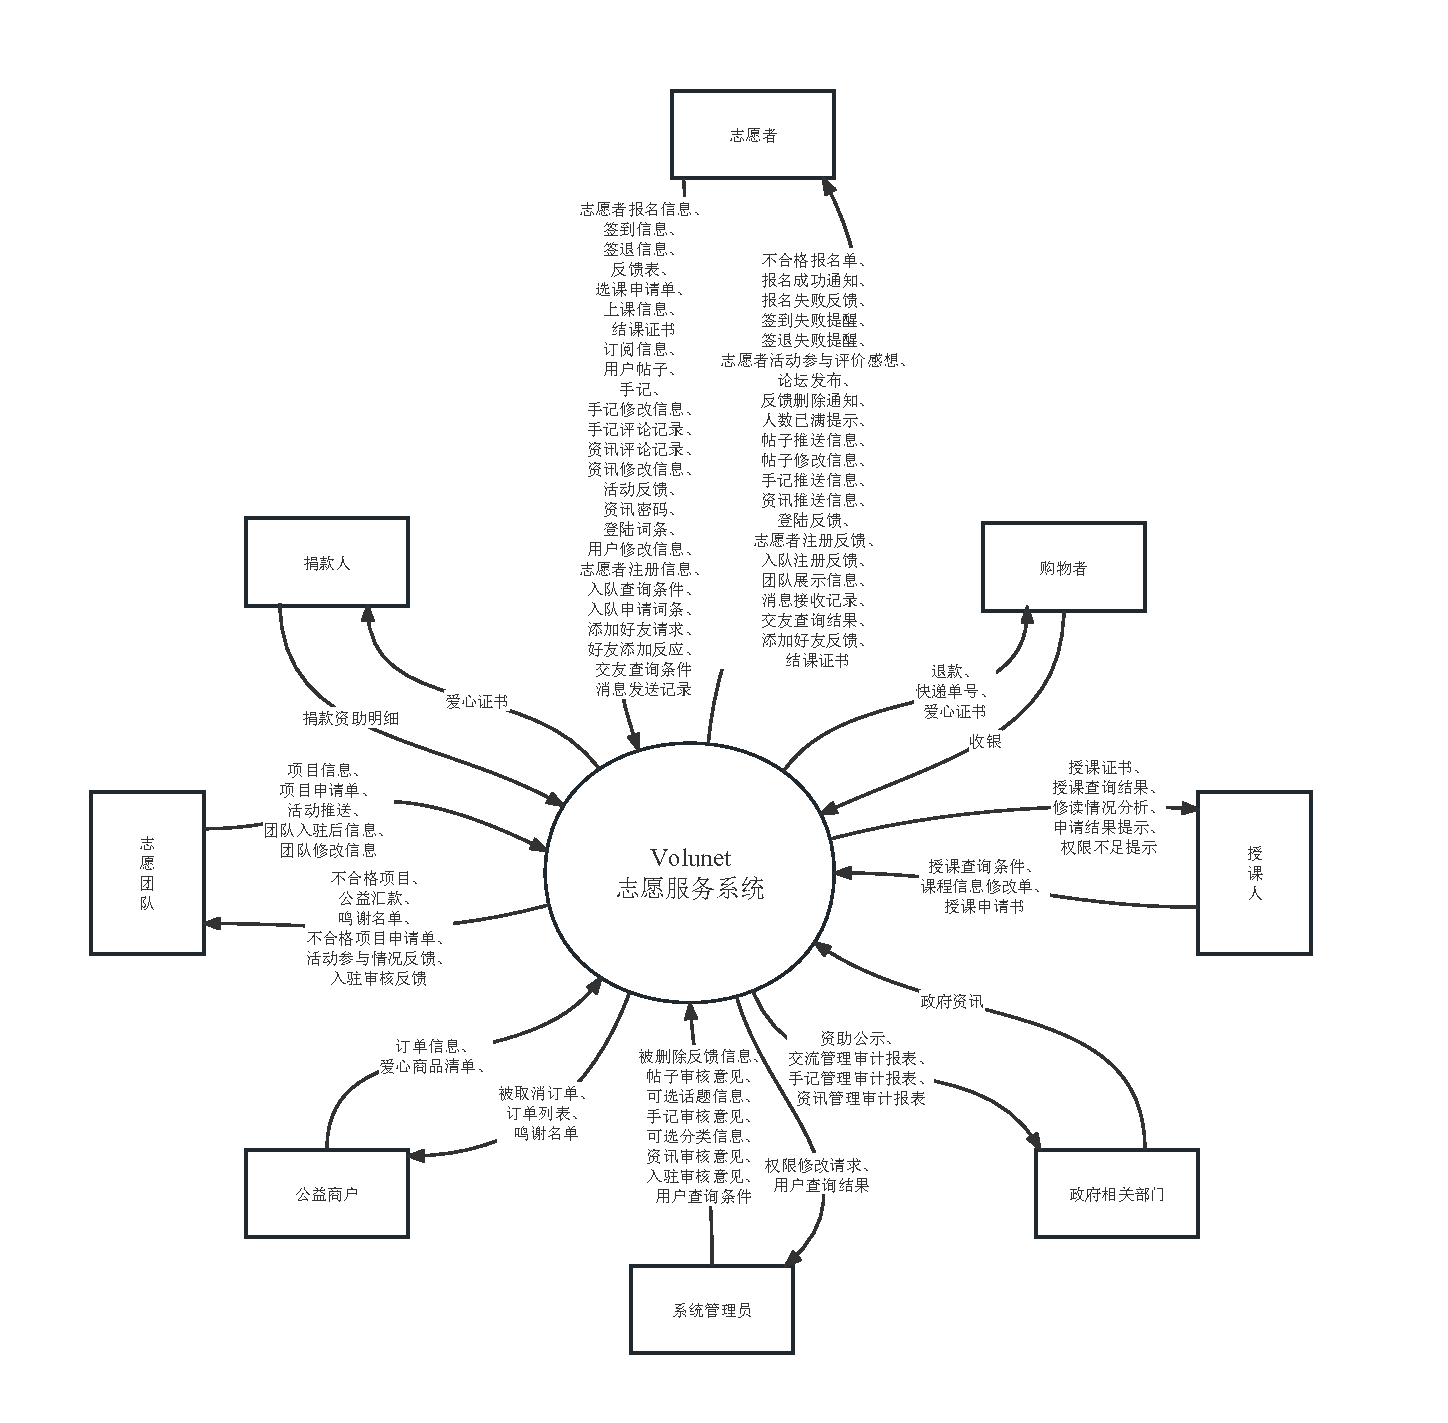
\includegraphics[width=0.95\textwidth]  {fig/top.pdf}} 
    \bicaption{Volunet顶层数据流图}{Top-level Data Flow Diagram of Volunet}
    \label{top_data}
    \end{figure}

\subsubsection{源点词条描述}

图\ref{top_data}的顶层数据流图中对应的源点词条描述如表\ref{tab_volunteer}-\ref{tab_government}所示。

\begin{table}[H]
  \begin{center}
    \caption{“志愿者”源点词条描述}
    %\setlength{\tabcolsep}{15mm}{
    \begin{tabular}{l p{11cm}} 
      \hline
      名称: & 志愿者\\
      \hline
      简述:& 进行志愿服务、课程学习、平台社交的用户\\
      \hline
    \end{tabular}
    \label{tab_volunteer}
  \end{center}
\end{table}


\begin{table}[H]
  \begin{center}
    \caption{“志愿团队”源点词条描述}
    %\setlength{\tabcolsep}{15mm}{
    \begin{tabular}{l p{11cm}} 
      \hline
      名称: & 志愿团队\\
      \hline
      简述:& 进行志愿发布、推送发布、接收捐款的用户\\
      \hline
    \end{tabular}
  \end{center}
\end{table}


\begin{table}[H]
  \begin{center}
    \caption{“公益商户”源点词条描述}
    %\setlength{\tabcolsep}{15mm}{
    \begin{tabular}{l p{11cm}} 
      \hline
      名称: & 公益商家\\
      \hline
      简述: & 进行商品提供、爱心鸣谢的用户\\
      \hline
    \end{tabular}
  \end{center}
\end{table}


\begin{table}[H]
  \begin{center}
    \caption{“购物者”源点词条描述}
    %\setlength{\tabcolsep}{15mm}{
    \begin{tabular}{l p{11cm}} 
      \hline
      名称: & 购物者\\
      \hline
      简述: & 进行商品购买、奉献爱心的用户\\
      \hline
    \end{tabular}
  \end{center}
\end{table}


\begin{table}[H]
  \begin{center}
    \caption{“捐款人”源点词条描述}
    %\setlength{\tabcolsep}{15mm}{
    \begin{tabular}{l p{11cm}} 
      \hline
      名称: & 捐助者\\
      \hline
      简述: & 进行项目资助、奉献爱心的用户\\
      \hline
    \end{tabular}
  \end{center}
\end{table}


\begin{table}[H]
  \begin{center}
    \caption{“授课人”源点词条描述}
    %\setlength{\tabcolsep}{15mm}{
    \begin{tabular}{l p{11cm}} 
      \hline
      名称: & 授课人\\
      \hline
      简述: & 进行课程讲授的用户\\
      \hline
    \end{tabular}
  \end{center}
\end{table}

\begin{table}[H]
  \begin{center}
    \caption{“系统管理员”源点词条描述}
    %\setlength{\tabcolsep}{15mm}{
    \begin{tabular}{l p{11cm}} 
      \hline
      名称: & 系统管理员\\
      \hline
      简述: & 进行内容审核、参数设置和权限管理的用户\\
      \hline
    \end{tabular}
    \label{tab_government}
  \end{center}
\end{table}

\begin{table}[H]
  \begin{center}
    \caption{“政府相关部门”源点词条描述}
    %\setlength{\tabcolsep}{15mm}{
    \begin{tabular}{l p{11cm}} 
      \hline
      名称: & 政府相关部门\\
      \hline
      简述: & 进行报表审阅、资讯提供的用户\\
      \hline
    \end{tabular}
    \label{tab_government}
  \end{center}
\end{table}


\subsubsection{数据项描述}

图\ref{top_data}的顶层数据流图中组成各数据流的数据项描述如表\ref{item_description}所示。

\begin{longtable}{p{3.5cm}llp{4cm}} 
        \caption{数据项描述} \\
        \hline 
        \multicolumn{1}{l}{\textbf{数据项名称}} & \multicolumn{1}{l}{\textbf{数据类型}} & \multicolumn{1}{l}{\textbf{计量单位}} & \multicolumn{1}{l}{\textbf{数据范围}}\\ 
        \hline 
        \endfirsthead
			
        \hline \multicolumn{1}{l}{\textbf{数据项名称}} & \multicolumn{1}{l}{\textbf{数据类型}} & \multicolumn{1}{l}{\textbf{计量单位}} & \multicolumn{1}{l}{\textbf{数据范围}}\\ \hline 
        \endhead
			
        \hline \multicolumn{4}{l}{{Continued on next page}} \\ 
        \endfoot
    			
        \hline
        \endlastfoot
        
        用户ID  & 整型  & 1 & 1..4294960000 \\ 
        用户名 & 字符串 & 字节 & \^[a-zA-Z0-9.]\{1,12\}\$ \\ 
        密码 & 字符串 & 字节 & \^[a-zA-Z0-9.]\{8,20\}\$ \\ 
        用户权限 & 整型  & 1 & 0..5 \\ 
         所属团队 & 整型  & 1 & 4294960001..4294967294 \\
        注册时间 & Unix 纪元时间 & 秒 & 0-4294967296 \\ 
        注册反馈信息字段 & 字符串 & 字节 & \^[a-zA-Z0-9.]\{1,200\}\$ \\
        登录反馈信息字段 & 字符串 & 字节 & \^[a-zA-Z0-9.]\{1,200\}\$ \\ 
        团队ID & 整型  & 1 & 4294960001..4294967295 \\ 
        团队名 & 字符串 & 字节 & \^[a-zA-Z0-9.]\{1,12\}\$ \\ 
        电子邮箱 & 字符串 & 字节 & \^[a-zA-Z0-9.\_\%+-]+@[a-zA-Z0-9.-]+$\backslash$.[a-zA-Z]\{2,\}\$ \\ 
        电话号码 & 字符串 & 字节 & \^$\backslash$+?$\backslash$d\{1,3\}[- ]?$\backslash$d\{3\}[- ]?$\backslash$d\{4\}\$ \\
        团队地址 & 字符串 & 字节 & \^[a-zA-Z0-9.]\{1,500\}\$ \\
        团队网站 & 字符串 & 字节 & \^(https?://)?([$\backslash$da-z.-]+)$\backslash$.([a-z.]\{2,6\})([/$\backslash$w .-]*)*/?\$ \\ 
        团队人数 & 整型  & 1 & 1..4294967295 \\
        团队名单 & 字符串 & 字节 & \^[a-zA-Z0-9.]\{1,2000\}\$ \\ 
        查询关键字 & 字符串 & 字节 & \^[a-zA-Z0-9.]\{1,50\}\$ \\ 
        查询时间 & Unix 纪元时间 & 秒 & 0-4294967296 \\ 
        入队审核反馈字段 & 字符串 & 字节 & \^$\backslash$w\{1,200\}\$ \\ 
        政府用户 ID & 整型  & 1 & 4294967295 \\ 
        政府家机构名 & 字符串 & 字节 & \^[a-zA-Z0-9.]\{1,12\}\$ \\ 
        资讯内容 & 二进制数据流 & 字节 & 有穷长度二进制组合 \\ 
        手记内容 & 二进制数据流 & 字节 & 有穷长度二进制组合 \\ 
        帖子内容 & 二进制数据流 & 字节 & 有穷长度二进制组合 \\ 
        修改内容 & 二进制数据流 & 字节 & 有穷长度二进制组合 \\ 
        资讯密码 & 字符串 & 字节 & \^[a-zA-Z0-9.]\{8,20\}\$ \\ 
        发布时间 & Unix 纪元时间 & 秒 & 0-4294967296 \\ 
        最后编辑时间 & Unix 纪元时间 & 秒 & 0-4294967296 \\ 
        类别 ID & 整型  & 1 & 1..256 \\ 
        话题 ID & 整型  & 1 & 1..256 \\ 
        类别名称 & 字符串 & 字节 & \^[a-zA-Z0-9.]\{1,12\}\$ \\ 
        话题名称 & 字符串 & 字节 & \^[a-zA-Z0-9.]\{1,12\}\$ \\ 
        修改要求 & 字符串 & 字节 & \^[a-zA-Z0-9.]\{1,500\}\$ \\
        审核情况 & 字符串 & 字节 & \^[a-zA-Z0-9.]\{1,50\}\$ \\ 
        评论 ID & 整型  & 1 & 1..4294967295 \\ 
        评论内容 & 字符串 & 字节 & \^[a-zA-Z0-9.]\{1,500\}\$ \\ 
        资讯审核信息统计分析报表字段 & 二进制数据流 & 字节 & 有穷长度二进制组合 \\
        手记审核信息统计分析报表字段 & 二进制数据流 & 字节 & 有穷长度二进制组合 \\ 
        帖子审核信息统计分析报表字段 & 二进制数据流 & 字节 & 有穷长度二进制组合 \\ 
        理由 & 字符串 & 字节 & \^[a-zA-Z0-9.]\{1,500\}\$ \\ 
        消息 ID & 整型  & 1 & 1..4294967295 \\ 
        消息内容 & 字符串 & 字节 & \^[a-zA-Z0-9.]\{1,50\}\$ \\ 
        志愿项目 ID & 整型  & 1 & 1..4294967295 \\
        订单 ID & 整型  & 1 & 1..4294967295 \\ 
        商品 ID & 整型  & 1 & 1..4294967295 \\ 
        公益商家 ID & 整型  & 1 & 1..4294967295 \\ 
        收件人 & 字符串 & 字节 & \^[a-zA-Z0-9.]\{1,12\}\$ \\ 
        联系方式 & 字符串 & 字节 & \^$\backslash$+?$\backslash$d\{1,3\}[- ]?$\backslash$d\{3\}[- ]?$\backslash$d\{4\}\$ \\
        发货地址 & 字符串 & 字节 & \^[a-zA-Z0-9.]\{1,500\}\$ \\
        下单时间 & Unix 纪元时间 & 秒 & 0-4294967296 \\ 
        付款金额 & 浮点型  & 0.01 & 0.00..1.8 x 10^308 \\ 
        支付方式 & 字符串 & 字节 & \^[a-zA-Z0-9.]\{1,10\}\$ \\ 
        快递公司 ID & 整型  & 1 & 1..4294967295 \\ 
        物流单号 ID & 整型  & 1 & 1..4294967295 \\ 
        完结时间 & Unix 纪元时间 & 秒 & 0-4294967296 \\ 
        感谢语 & 字符串 & 字节 & \^[a-zA-Z0-9.]\{1,100\}\$ \\ 
        证书生成时间 & Unix 纪元时间 & 秒 & 0-4294967296 \\ 
        证明文字 & 字符串 & 字节 & \^[a-zA-Z0-9.]\{1,100\}\$ \\ 
        捐款金额 & 浮点型  & 0.01 & 0.00..1.8 x 10^308 \\ 
        项目时间 & Unix 纪元时间 & 秒 & 0-4294967296 \\
        可报名人数 & 整型  & 1 & 1..4294967295 \\ 
        项目描述 & 字符串 & 字节 & \^[a-zA-Z0-9.]\{1,200\}\$ \\ 
        捐款留言 & 字符串 & 字节 & \^[a-zA-Z0-9.]\{1,100\}\$ \\ 
        资助金额 & 浮点型  & 0.01 & 0.00..1.8 x 10^308 \\ 
        \label{item_description}
\end{longtable}

\subsection{0层数据流图} 
进一步细化Volunt志愿服务系统的各个加工步骤说明,下面给出Volunt志愿服务系统的0层数据图(图\ref{0_level_data}),包括信息管理、志愿服务、爱心捐助、公益课程、交流论坛、志愿交友在内的6个更细的数据流加工。

\begin{figure}[H]
  \centering
  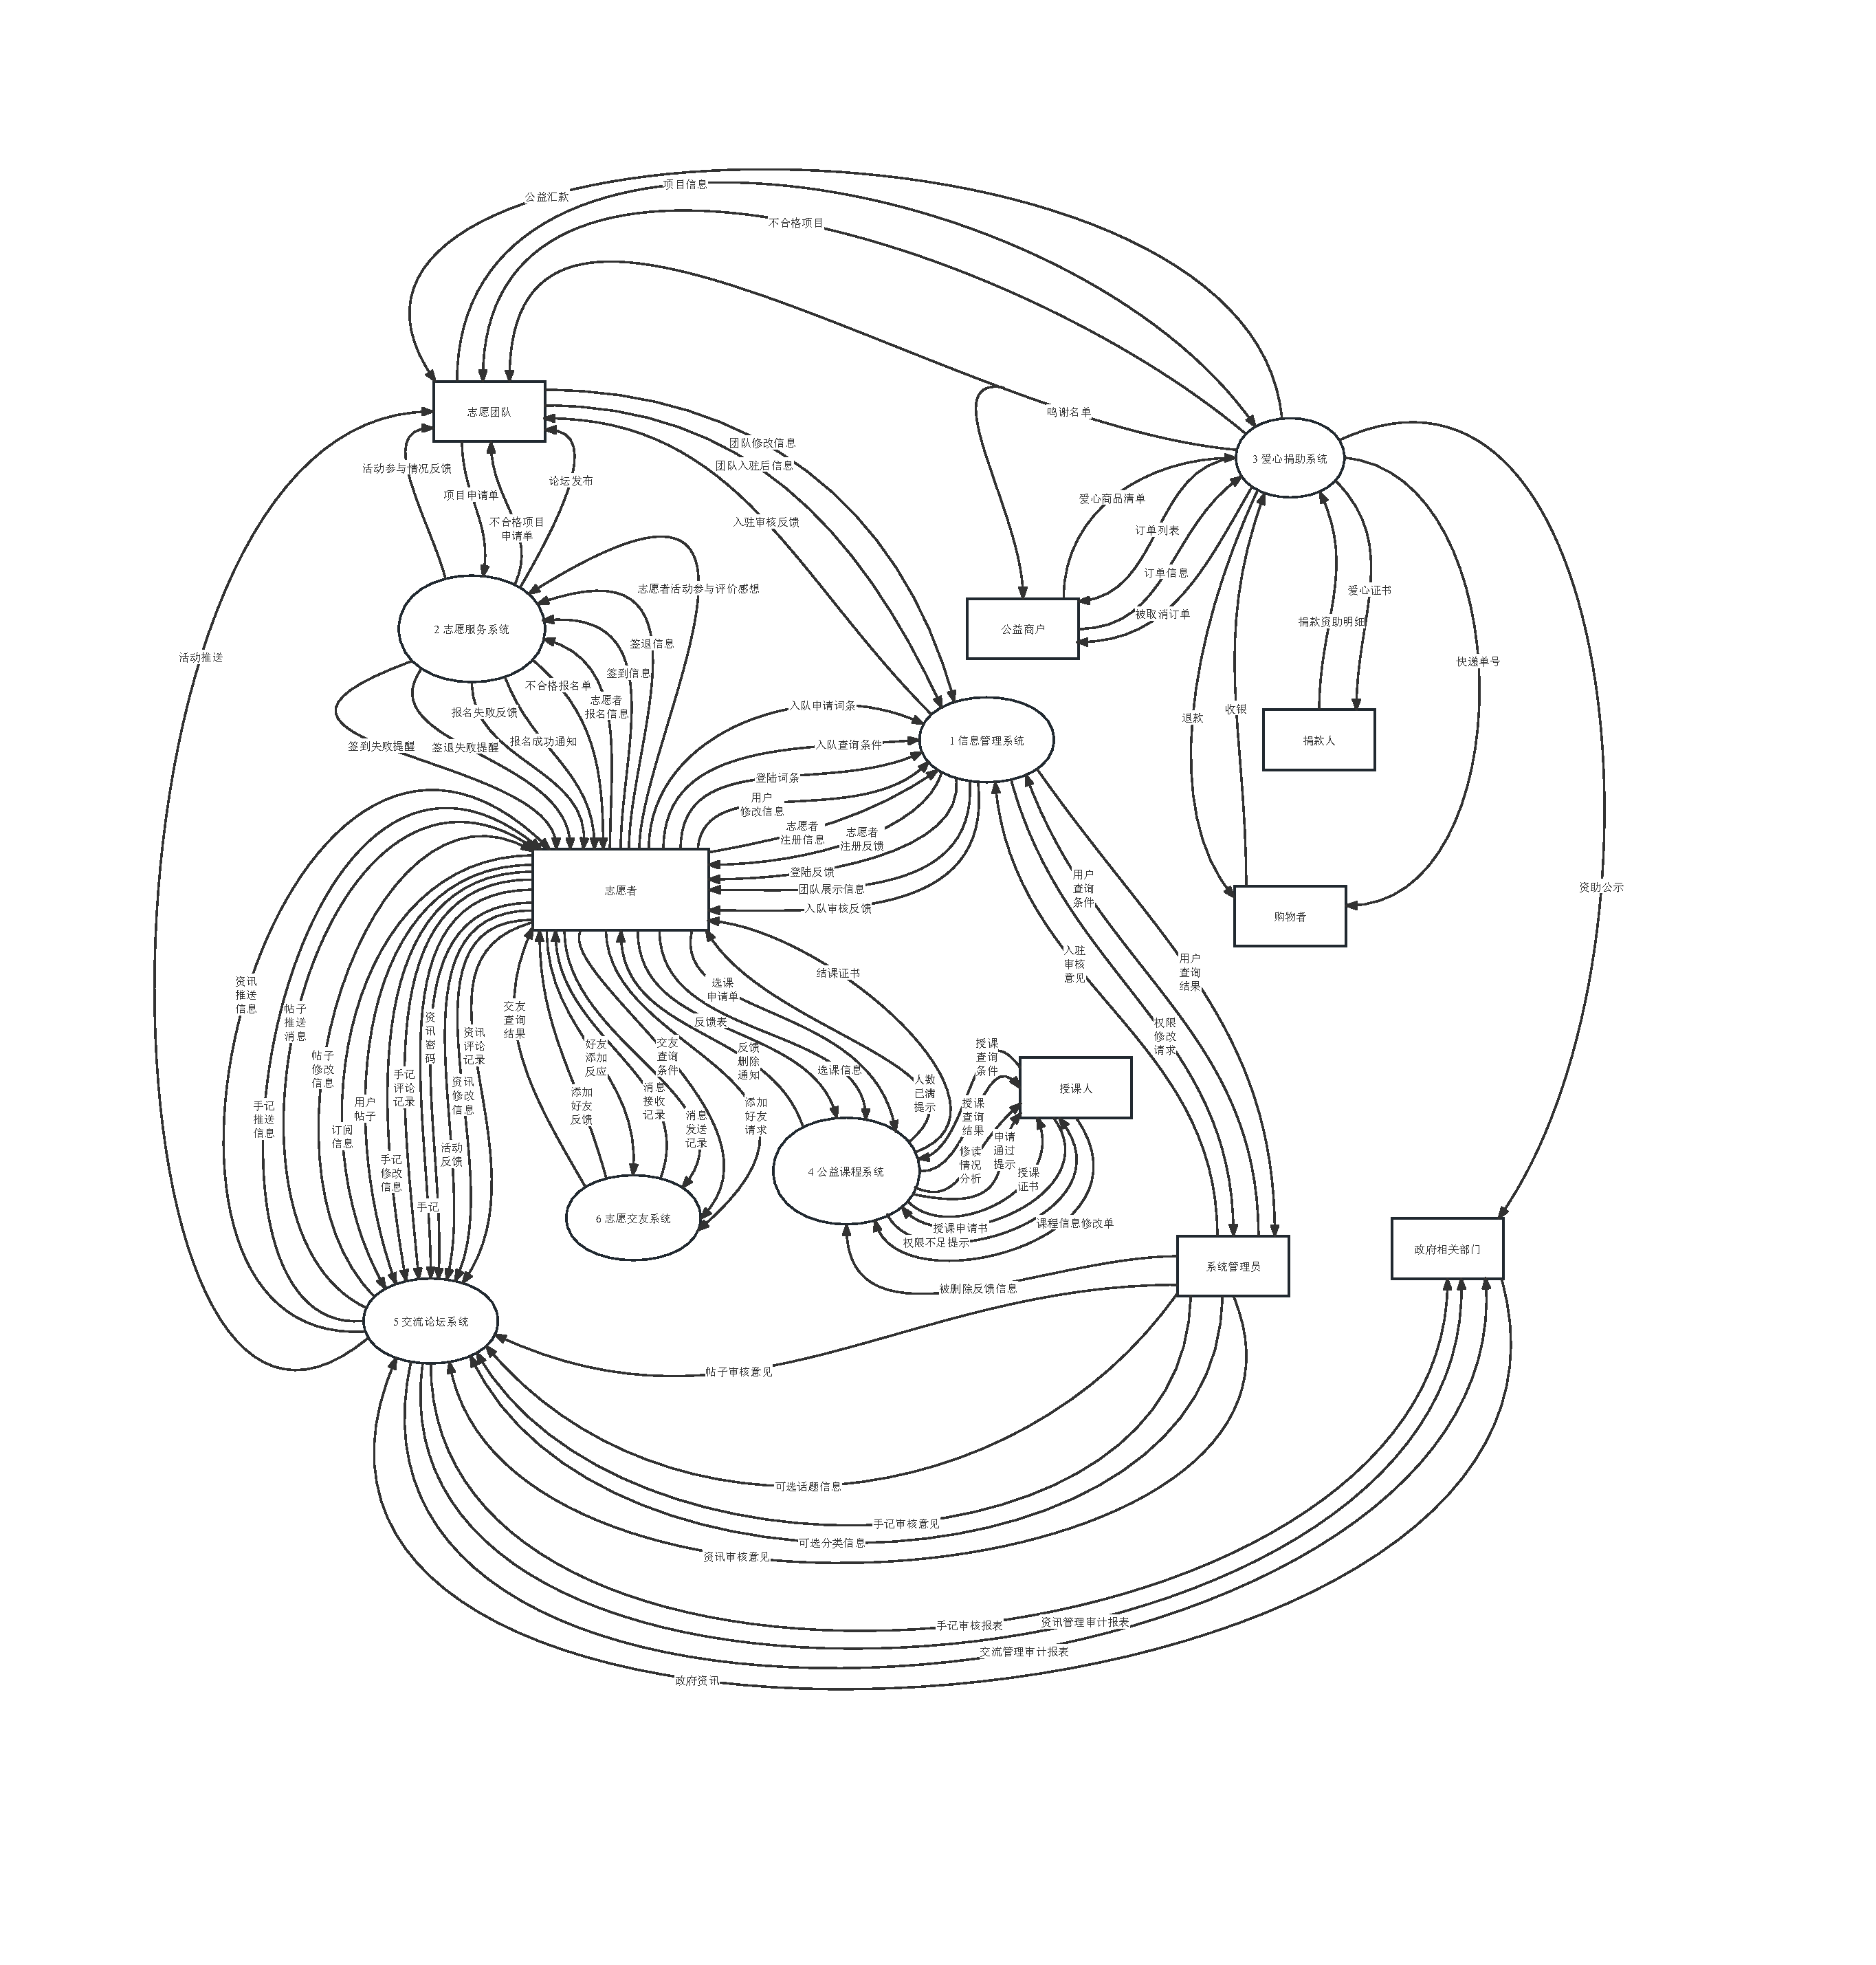
\includegraphics[width=\textwidth, height=0.95\textheight]{SAD/fig/0_level.pdf}
  \bicaption{Volunet0层数据流图}{Data Flow Diagram for Level 0 of Volunet}
  \label{0_level_data}
\end{figure}
  
\subsubsection{数据加工词条描述说明}
\begin{table}[H]  
\caption{“信息管理系统”加工词条描述}  
\begin{center}  
    \begin{tabular}{l p{11cm}} 
        \hline
        \quad 名称:  &   信息管理系统 \\
        \hline
        \quad 编号:  & 1 \\
        \hline
        \quad 简述:  & 处理志愿者的注册登录,志愿团队的入驻,志愿者加入团队及系统管理员对相关信息的管理的功能 \\
        \hline
        \quad 输入:  & 入队申请词条、入队查询条件、登录词条、用户修改信息、志愿者注册信息、团队入驻信息、团队修改信息、入队审核意见、用户查询词条、权限修改请求 \\
        \hline
        \quad 输出:  & 入队审核反馈、登陆反馈、团队展示信息、志愿者注册反馈、入驻审核反馈、用户查询结果 \\
        \hline
        \quad 逻辑:  & 根据入队申请词条处理申请,根据团队入驻信息处理入驻,根据系统管理员的审核意见通过或驳回申请。根据登录词条处理用户登录。根据用户查询词条返回用户查询结果。根据权限修改请求修改用户权限。 \\
        \hline
        \quad 异常处理: & 接收到的信息不符合数据项描述的规则,则拒绝处理。用户注册信息不合格,则返回入队审核反馈提醒用户不合格部分。团队入驻信息审核不合格,则返回驻审核反馈提醒团队错不合格部分。\\ 
        \hline
        \quad 加工激发条件: & 接到输入数据 \\ 
        \hline
    \end{tabular}
    \label{tab1}
\end{center}
\end{table}


\begin{table}[H]  
\caption{“志愿服务系统”加工词条描述}  
\begin{center}  
    \begin{tabular}{l p{11cm}} 
        \hline
        \quad 名称:  &   志愿服务系统 \\
        \hline
        \quad 编号:  & 2 \\
        \hline
        \quad 简述:  & 处理志愿团队申报志愿项目,志愿者报名参与志愿项目,志愿团队选择志愿者并在过程中对志愿者签到签退信息进行管理,志愿者在活动结束提供反馈的功能 \\
        \hline
        \quad 输入:  & 项目申请单、志愿者报名单、签到信息、签退信息、志愿者活动评价反馈信息、 \\
        \hline
        \quad 输出:  & 不合格项目申请单、不合格报名单、报名成功通知、报名失败反馈、签到失败提醒、签退失败提醒、活动参与情况反馈、论坛发布 \\
        \hline
        \quad 逻辑:  & 根据支援团队提交项目申报单处理申请,根据志愿者报名单处理志愿者报名信息,再交由志愿团队选择,根据志愿团队选择结果向志愿者发送报名成功通知或报名失败信息。根据志愿者签到、签退、评价反馈生成志愿者活动报告交由志愿团队。 \\
        \hline
        \quad 异常处理: & 接收到的信息不符合数据项描述的规则,则拒绝处理。志愿项目申请单不合格,则返回不合格申请单提醒用户不合格部分。志愿者报名单审核不合格,则返回不合格报名单提醒志愿者不合格部分。签到信息、签退信息、反馈信息不合格,则返回相对应的不合格信息交由志愿者。\\ 
        \hline
        \quad 加工激发条件: & 接到输入数据 \\ 
        \hline
    \end{tabular}
    \label{tab1}
\end{center}
\end{table}


\begin{table}[H]  
\caption{“爱心捐助系统”加工词条描述}  
\begin{center}  
    \begin{tabular}{l p{11cm}} 
        \hline
        \quad 名称:  &   爱心捐助系统 \\
        \hline
        \quad 编号:  & 3 \\
        \hline
        \quad 简述:  & 处理爱心商品的交易,志愿项目的捐款和爱心反馈的管理以及相关财务报表送审的功能 \\
        \hline
        \quad 输入:  & 项目信息、爱心商品清单、订单信息、收银、捐款资助明细 \\
        \hline
        \quad 输出:  & 不合格项目、公益汇款、鸣谢名单、订单列表、被取消订单、退款、爱心证书、快递单号、资助公示 \\
        \hline
        \quad 逻辑:  & 根据订单信息处理订单和货款。根据项目信息处理项目资助审核,根据系统管理员的审核通过或驳回资助申请。根据捐款资助明细处理爱心人士捐款。再根据上述过程得到的爱心人士信息处理爱心反馈。 \\
        \hline
        \quad 异常处理: & 接收到的信息不符合数据项描述的规则,则拒绝处理。当接受到的项目信息审核不通过会驳回,当订单被取消则会被退回并退款。\\ 
        \hline
        \quad 加工激发条件: & 接到输入数据 \\ 
        \hline
    \end{tabular}
    \label{tab1}
\end{center}
\end{table}

\begin{table}[H]  
\caption{“公益课程系统”加工词条描述}  
\begin{center}  
    \begin{tabular}{l p{11cm}} 
        \hline
        \quad 名称:  &   公益课程系统 \\
        \hline
        \quad 编号:  & 4 \\
        \hline
        \quad 简述:  & 处理用户学习课程、授课人教授课程和管理员维护课程的功能  \\
        \hline
        \quad 输入:  & 反馈表、选课信息、选课申请单、消息发送记录、授课查询条件、授课申请书 \\
        \hline
        \quad 输出:  & 反馈删除通知、人数已满提示,结课证书、授课查询结果、修读情况分析、申请通过提示、授课证书、权限不足提示 \\
        \hline
        \quad 逻辑:  & 根据授课查询条件检索返回申请通过情况,并对相应课程进行处理。根据选课查询条件检索课程,返回查询课程信息。根据反馈信息,处理反馈信息,发送反馈处理通知给相应用户 \\
        \hline
        \quad 异常处理: & 反馈格式、修读情况日期、证书版式不符合数据项的描述规则,则拒绝处理。\\ 
        \hline
        \quad 加工激发条件: & 接到输入数据 \\ 
        \hline
    \end{tabular}
    \label{tab1}
\end{center}
\end{table}

\begin{table}[H]  
\caption{“交流论坛系统”加工词条描述}  
\begin{center}  
    \begin{tabular}{l p{11cm}} 
        \hline
        \quad 名称:  &   交流论坛系统 \\
        \hline
        \quad 编号:  & 5 \\
        \hline
        \quad 简述:  & 处理志愿者、志愿团队、政府机构发布资讯,志愿者发布手记、帖子和评论及相关信息审核审计的功能 \\
        \hline
        \quad 输入:  & 资讯评论记录、资讯修改信息、活动反馈、资讯密码、可选分类信息、资讯审核意见、政府资讯、活动推送、手记修改信息、手记、手记评论记录、手记推送信息、手记审核意见、订阅信息、用户帖子、帖子审核意见、可选话题信息 \\
        \hline
        \quad 输出:  & 资讯推送信息、资讯管理审计报表、手记推送信息、手记管理审计报表、帖子推送信息、帖子修改信息、交流管理审计报表 \\
        \hline
        \quad 逻辑:  & 在资讯、手记、交流三个板块,接收提交的信息并处理审核发布。接收针对信息的评论。最后根据所有信息生成推送信息和审核报表。 \\
        \hline
        \quad 异常处理: & 接收到的信息不符合数据项描述的规则,则拒绝处理。当接受到的信息审核不通过会驳回。\\ 
        \hline
        \quad 加工激发条件: & 接到输入数据 \\ 
        \hline
    \end{tabular}
    \label{tab1}
\end{center}
\end{table}

\begin{table}[H]  
\caption{“志愿交友系统”加工词条描述}  
\begin{center}  
    \begin{tabular}{l p{11cm}} 
        \hline
        \quad 名称:  &   志愿交友系统 \\
        \hline
        \quad 编号:  & 6 \\
        \hline
        \quad 简述:  & 处理用户交友和私聊的功能  \\
        \hline
        \quad 输入:  & 交友查询条件、添加好友请求、好友添加反应、消息发送记录 \\
        \hline
        \quad 输出:  & 交友查询结果、添加好友反馈,消息接受记录 \\
        \hline
        \quad 逻辑:  & 根据交友查询条件检索返回查询结果列表。根据添加好友请求,及用户的反应进行处理,并返回反馈。根据消息发送记录,发送消息接受记录给对应好友。 \\
        \hline
        \quad 异常处理: & 查询条件、消息发送记录不符合数据项描述的规则,则拒绝处理。\\ 
        \hline
        \quad 加工激发条件: & 接到输入数据 \\ 
        \hline
    \end{tabular}
    \label{tab1}
\end{center}
\end{table}



% \begin{table}[H]  
% \caption{“公益课程系统”加工词条描述}  
% \begin{center}  
%     \begin{tabular}{l p{11cm}} 
%         \hline
%         \quad 名称:  &   公益课程系统 \\
%         \hline
%         \quad 编号:  & 7 \\
%         \hline
%         \quad 简述:  & 处理用户学习课程、授课人教授课程和管理员维护课程的功能  \\
%         \hline
%         \quad 输入:  & 反馈表、选课信息、选课申请单、消息发送记录、授课查询条件、授课申请书 \\
%         \hline
%         \quad 输出:  & 反馈删除通知、人数已满提示,结课证书、授课查询结果、修读情况分析、申请通过提示、授课证书、权限不足提示 \\
%         \hline
%         \quad 逻辑:  & 根据授课查询条件检索返回申请通过情况,并对相应课程进行处理。根据选课查询条件检索课程,返回查询课程信息。根据反馈信息,处理反馈信息,发送反馈处理通知给相应用户 \\
%         \hline
%         \quad 异常处理: & 反馈格式、修读情况日期、证书版式不符合数据项的描述规则,则拒绝处理。\\ 
%         \hline
%         \quad 加工激发条件: & 接到输入数据 \\ 
%         \hline
%     \end{tabular}
%     \label{tab1}
% \end{center}
% \end{table}

\subsection{1层数据流图}   
在0层数据流图的基础上,本节将分析volunet志愿服务系统的1层数据流图,同样分为信息管理系统、志愿服务系统、爱心管理系统、公益课程系统、交流论坛系统、志愿交友系统六个部分进行介绍。

\subsubsection{信息管理系统}
以下是信息管理系统的1层数据流图、加工子图以及对应的数据字典和文件。信息管理系统分为个人管理、登陆管理、团队管理、用户管理和组队管理。
\begin{figure}[H]
    \center{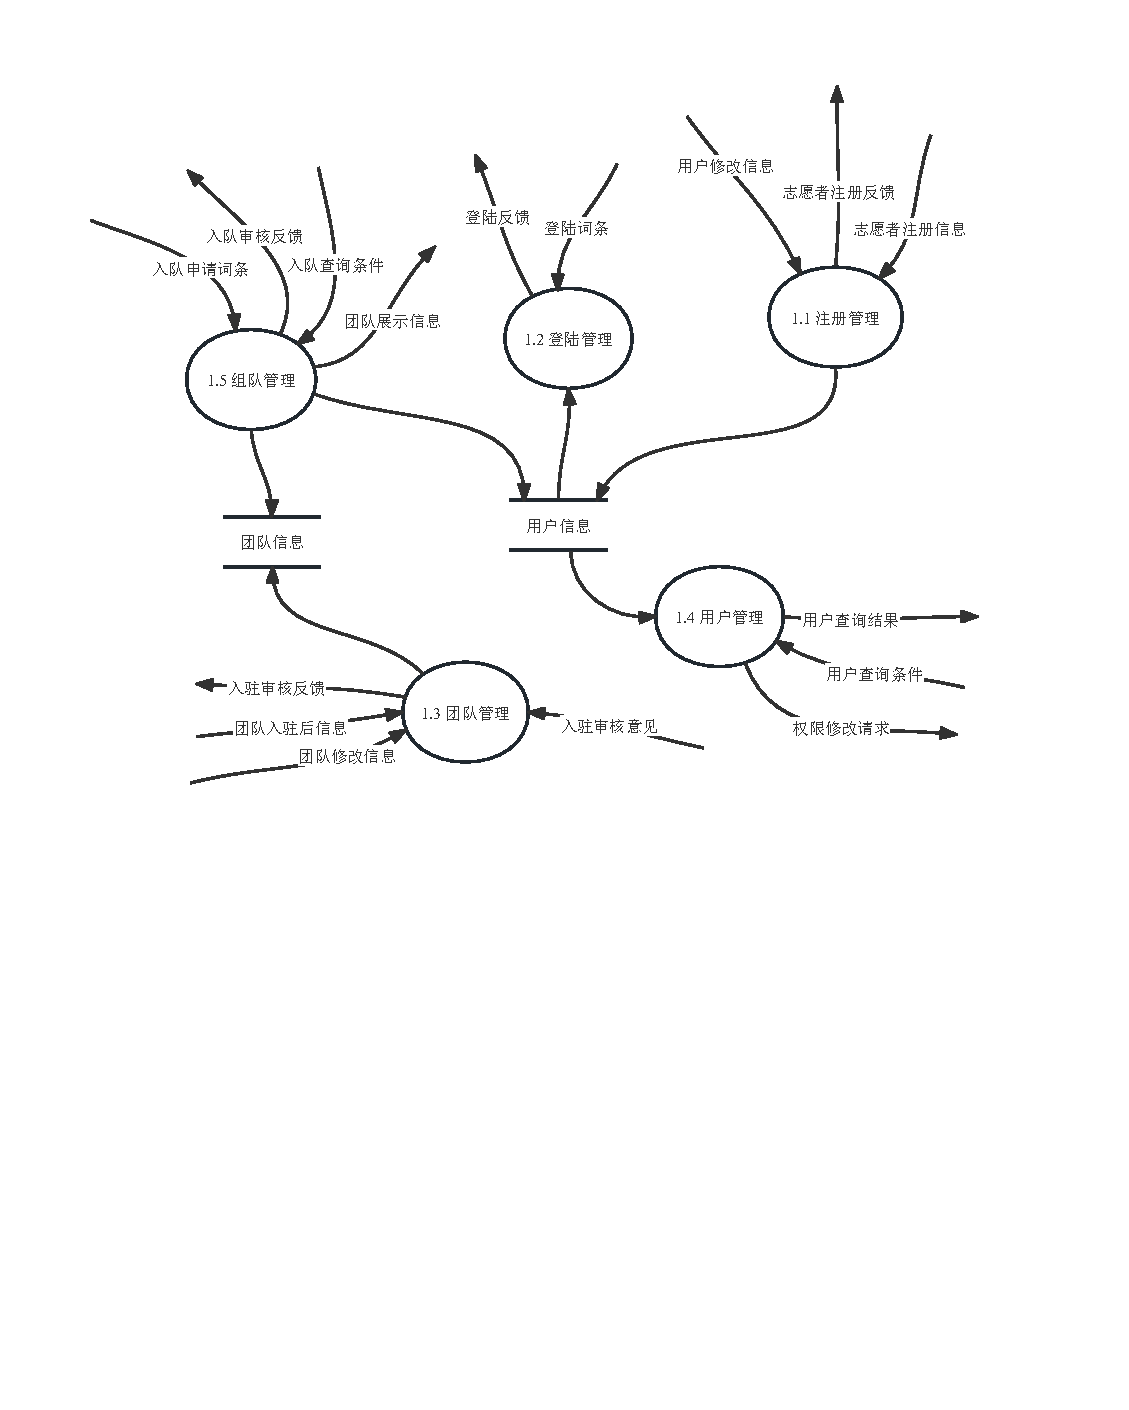
\includegraphics[width=0.95\textwidth]  {fig/信息管理/I_1.pdf}} 
    \bicaption{信息管理系统1层数据流图}{Data Flow Diagram for Level 1 of Information Management System}
    \end{figure}

\paragraph{个人管理}~{}
\\


\begin{figure}[H]
    \center{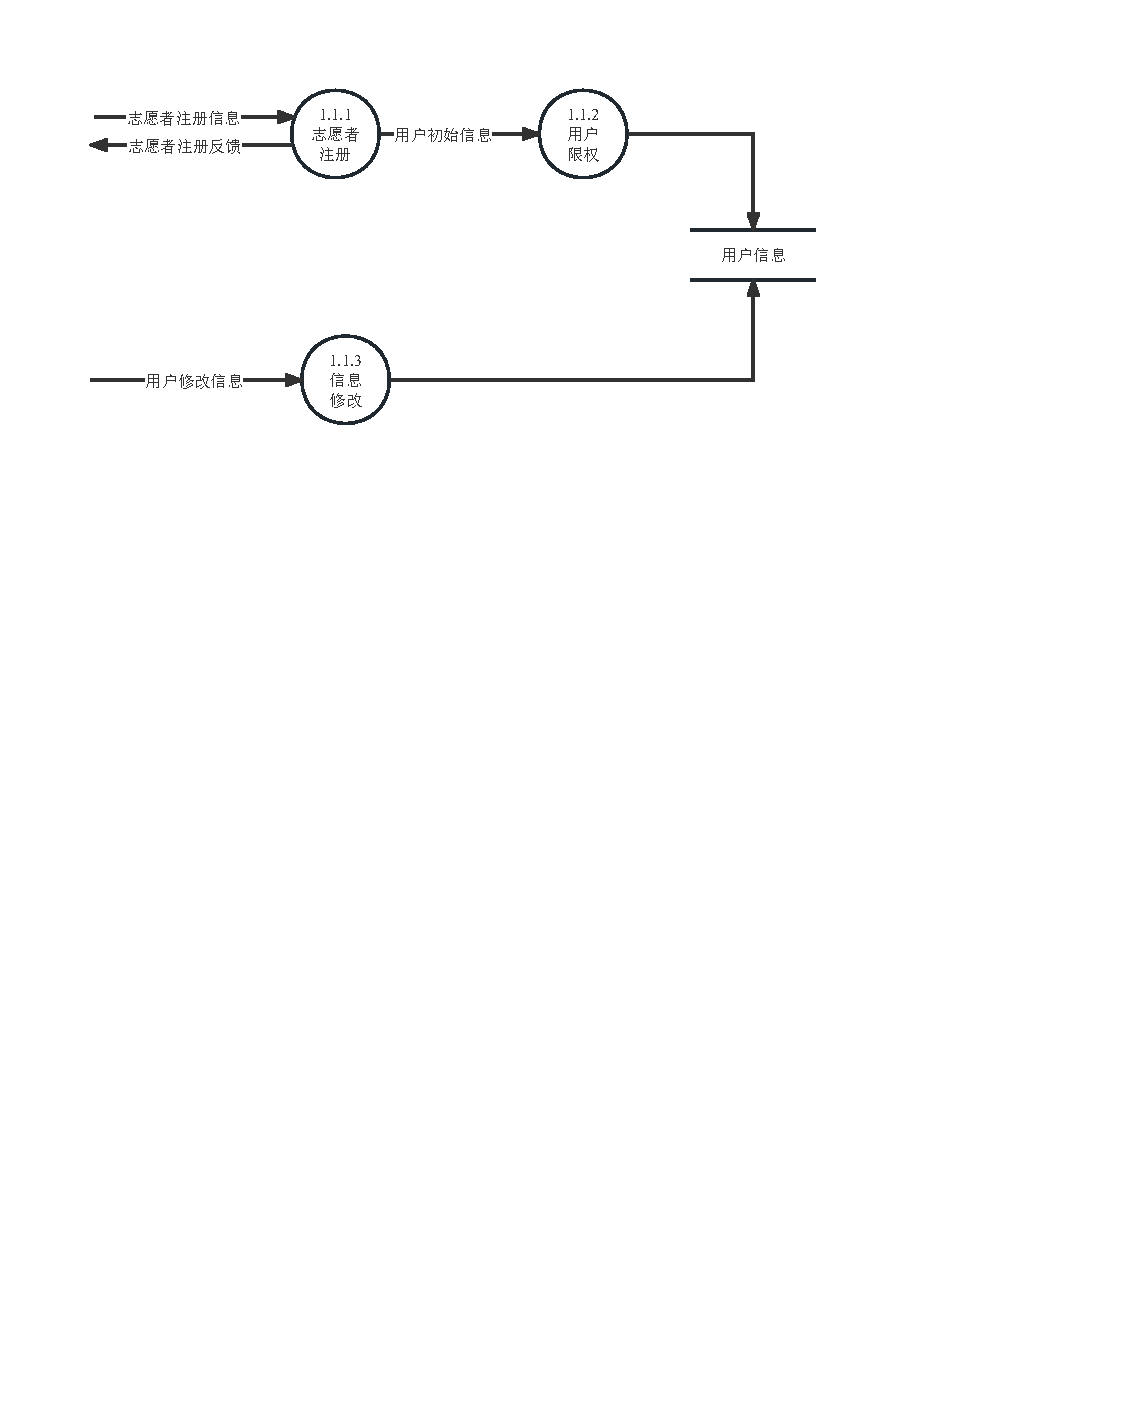
\includegraphics[width=0.95\textwidth]  {fig/信息管理/I_2-1.pdf}} 
    \bicaption{信息管理系统2层数据流图}{Data Flow Diagram for Level 2 of Information Management System}
    \end{figure}

(1)数据加工词条描述说明
\begin{table}[H]  
\caption{“志愿者注册”加工词条描述}  
\begin{center}  
    \begin{tabular}{l p{11cm}} 
        \hline
        \quad 名称:  &   注册填写 \\
        \hline
        \quad 编号:  & 1.1.1 \\
        \hline
        \quad 简述:  & 生成供审核的用户初始信息 \\
        \hline
        \quad 输入:  & 志愿者注册信息 \\
        \hline
        \quad 输出:  & 用户初始信息、志愿者注册反馈\\
        \hline
        \quad 逻辑:  & 根据志愿者注册信息生成用户初始信息,志愿者注册反馈。 \\
        \hline
    \end{tabular}
    \label{tab1}
\end{center}
\end{table}

\begin{algorithm}[H]
    \renewcommand{\thealgorithm}{}
    \caption{“志愿者注册”加工小说明} 
    \label{alg3} 
    \begin{algorithmic}[1]
        \IF{Pass Check 志愿者注册信息} 
        \STATE Create 用户ID
        \STATE Get 系统时间 As 注册时间
        \STATE Generate 注册反馈信息字段 Based On 志愿者注册信息
        \STATE Write 志愿者注册信息 + 用户ID + 注册时间 To 用户初始信息
        \STATE Write 注册反馈信息字段  To 志愿者注册反馈 
        \ELSE
        \STATE Generate 注册反馈信息字段 Based on 志愿者注册信息
        \STATE Write 注册反馈信息字段 To 志愿者注册反馈 
        \ENDIF 
    \end{algorithmic} 
\end{algorithm}

\begin{table}[H]  
\caption{“初始限权”加工词条描述}  
\begin{center}  
    \begin{tabular}{l p{11cm}} 
        \hline
        \quad 名称:  &   初始限权 \\
        \hline
        \quad 编号:  & 1.1.2 \\
        \hline
        \quad 简述:  & 为用户出示化权限的功能 \\
        \hline
        \quad 输入:  & 用户初始信息 \\
        \hline
        \quad 输出:  & 用户信息 \\
        \hline
        \quad 逻辑:  & 根据用户初始信息赋予权限生成完整的用户信息。 \\
        \hline
    \end{tabular}
    \label{tab1}
\end{center}
\end{table}

\begin{algorithm}[H] 
    \renewcommand{\thealgorithm}{}
    \caption{“初始限权”加工小说明} 
    \label{alg3} 
    \begin{algorithmic}[1]
        \STATE Generate 用户权限 Based On 用户初始信息
        \STATE Write 用户初始信息 + 用户权限 To 用户信息 
    \end{algorithmic} 
\end{algorithm}

\begin{table}[H]  
\caption{“信息修改”加工词条描述}  
\begin{center}  
    \begin{tabular}{l p{11cm}} 
        \hline
        \quad 名称:  &   信息修改 \\
        \hline
        \quad 编号:  & 1.1.3 \\
        \hline
        \quad 简述:  & 对用户信息进行修改的功能 \\
        \hline
        \quad 输入:  & 用户修改信息 \\
        \hline
        \quad 输出:  & 用户信息 \\
        \hline
        \quad 逻辑:  & 完成用户修改信息的处理。 \\
        \hline
    \end{tabular}
    \label{tab1}
\end{center}
\end{table}

\begin{algorithm}[H] 
    \renewcommand{\thealgorithm}{}
    \caption{“信息修改”加工小说明} 
    \label{alg3} 
    \begin{algorithmic}[1]
        \STATE Update 用户修改信息 In 用户信息 Match 用户ID
    \end{algorithmic} 
\end{algorithm}

(2)数据流词条描述说明
\begin{table}[H]  
\caption{``志愿者注册信息"数据流词条描述}  
\begin{center}  
    \begin{tabular}{l p{11cm}} 
        \hline
        \quad 名称:  &   志愿者注册信息 \\
        \hline
        \quad 简述:  & 志愿者为注册输入的信息 \\
        \hline
        \quad 来源:  & 源点``志愿者"\\
        \hline
        \quad 去向:  & 加工``志愿者注册" \\
        \hline
        \quad 组成:  & 用户名+账号+密码 \\
        \hline
    \end{tabular}
    \label{tab1}
\end{center}
\end{table}

\begin{table}[H]  
\caption{``志愿者注册反馈"数据流词条描述}  
\begin{center}  
    \begin{tabular}{l p{11cm}} 
        \hline
        \quad 名称:  &   志愿者注册反馈 \\
        \hline
        \quad 简述:  & 团队为注册输入信息 \\
        \hline
        \quad 来源:  & 加工``志愿者注册"\\
        \hline
        \quad 去向:  & 源点``志愿者" \\
        \hline
        \quad 组成:  & 注册反馈信息字段 \\
        \hline
    \end{tabular}
    \label{tab1}
\end{center}
\end{table}

\begin{table}[H]  
\caption{``用户初始信息"数据流词条描述}  
\begin{center}  
    \begin{tabular}{l p{11cm}} 
        \hline
        \quad 名称:  &   用户初始信息 \\
        \hline
        \quad 简述:  & 根据志愿者输入初始化的信息 \\
        \hline
        \quad 来源:  & 加工``志愿者注册"\\
        \hline
        \quad 去向:  & 加工``用户限权" \\
        \hline
        \quad 组成:  & 用户ID+用户名+账号+密码+所属团队+注册时间 \\
        \hline
    \end{tabular}
    \label{tab1}
\end{center}
\end{table}

\begin{table}[H]  
\caption{``用户修改信息"数据流词条描述}  
\begin{center}  
    \begin{tabular}{l p{11cm}} 
        \hline
        \quad 名称:  &   用户修改信息 \\
        \hline
        \quad 简述:  & 用户修改后的个人信息 \\
        \hline
        \quad 来源:  & 源点``志愿者"\\
        \hline
        \quad 去向:  & 加工``信息修改" \\
        \hline
        \quad 组成:  & 用户ID +用户名+密码 \\
        \hline
    \end{tabular}
    \label{tab1}
\end{center}
\end{table}

(3)文件词条描述
\begin{table}[H]  
\caption{“用户信息”文件词条描述}  
\begin{center}  
    \begin{tabular}{l p{10cm}} 
        \hline
        \quad 名称:  &  用户信息 \\
        \hline
        \quad 简述:  & 存储用户信息内容\\
        \hline
        \quad 组成:  & 用户ID+用户名+账号+密码+用户权限+所属团队+注册时间 \\
        \hline
        \quad 存储方式:  & 以用户ID为关键字。 \\
        \hline
    \end{tabular}
    \label{tab1}
\end{center}
\end{table}


\paragraph{登陆管理}~{}
\\

\begin{figure}[H]
    \center{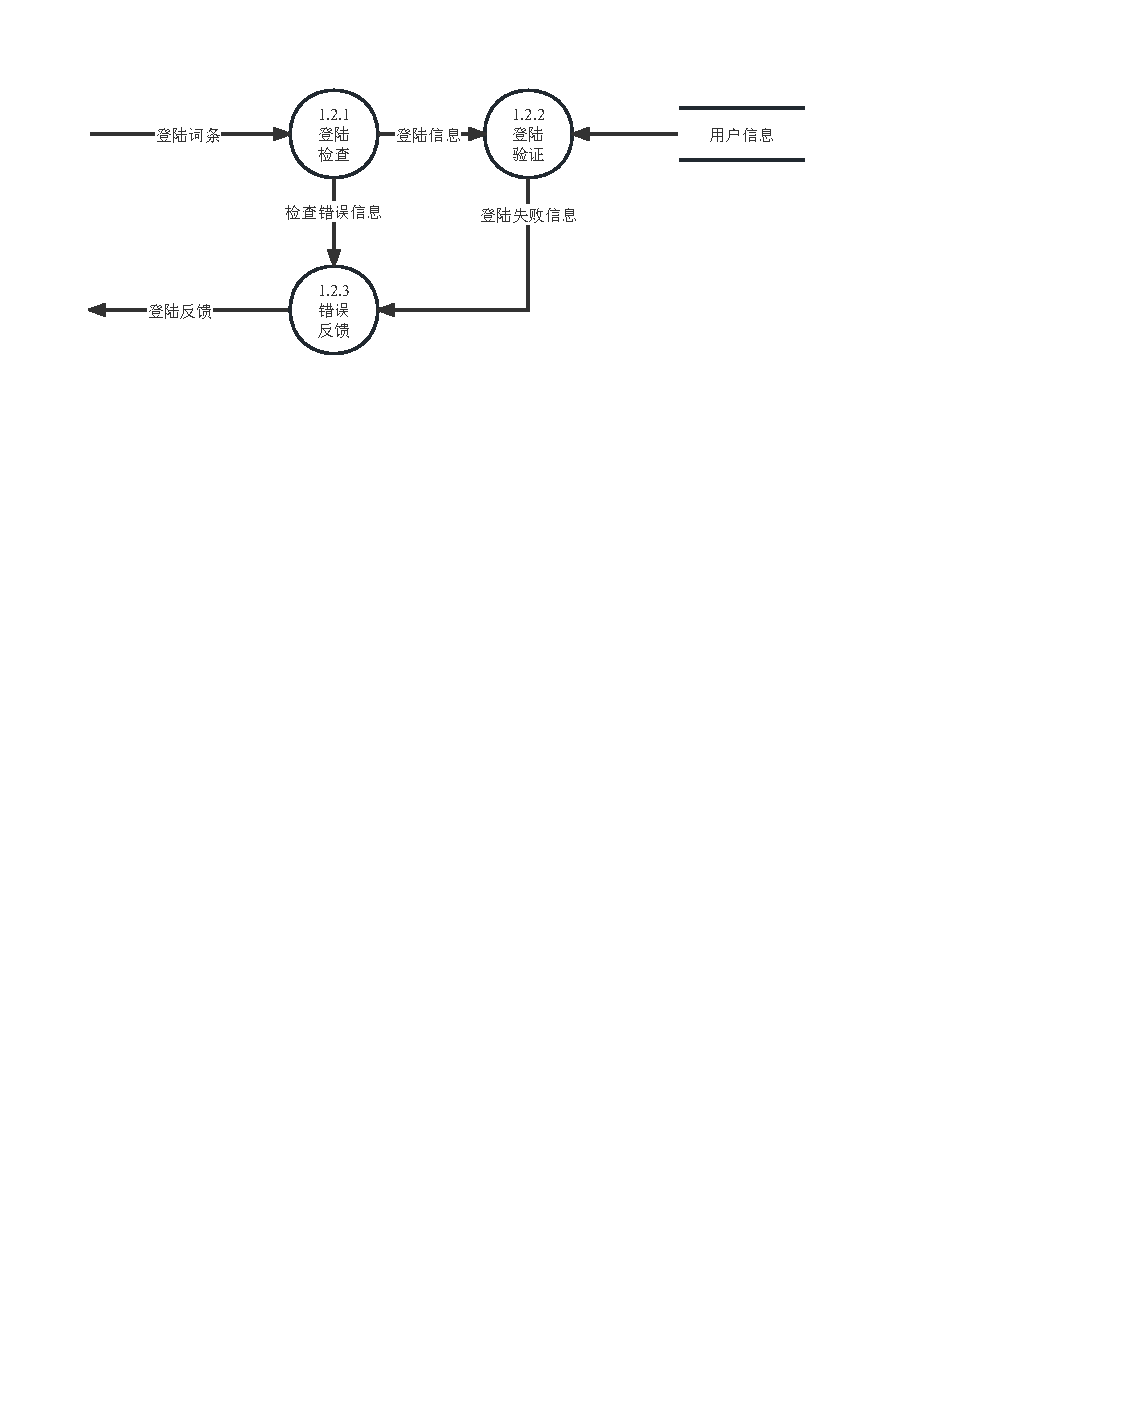
\includegraphics[width=0.95\textwidth]  {fig/信息管理/I_2-2.pdf}} 
    \bicaption{信息管理系统2层数据流图}{Data Flow Diagram for Level 2 of Information Management System}
    \label{0level_data}
    \end{figure}

(1)数据加工词条描述说明
\begin{table}[H]  
\caption{“登陆检查”加工词条描述}  
\begin{center}  
    \begin{tabular}{l p{11cm}} 
        \hline
        \quad 名称:  &   登陆检查 \\
        \hline
        \quad 编号:  & 1.2.1 \\
        \hline
        \quad 简述:  & 检查用户登陆词条是够正确的功能 \\
        \hline
        \quad 输入:  & 登陆词条\\
        \hline
        \quad 输出:  & 登陆信息\\
        \hline
        \quad 逻辑:  & 检查用户登陆词条是够正确,并根据用户填写的登陆词条生成登陆信息。 \\
        \hline
    \end{tabular}
    \label{tab1}
\end{center}
\end{table}

\begin{algorithm}[H]
    \renewcommand{\thealgorithm}{}
    \caption{“登陆检查”加工小说明} 
    \label{alg3} 
    \begin{algorithmic}[1]
        \IF{Pass Check 登陆词条} 
        \STATE Get 系统时间 As 登陆时间
        \STATE Write 登陆词条 + 登陆时间 To 登陆信息
        \ELSE
        \STATE Generate 检查错误信息字段 Based on 登陆词条
        \STATE Write 检查错误信息字段 To 错误检查信息 
        \ENDIF 
    \end{algorithmic} 
\end{algorithm}

\begin{table}[H]  
\caption{“登陆验证”加工词条描述}  
\begin{center}  
    \begin{tabular}{l p{11cm}} 
        \hline
        \quad 名称:  &   登陆验证 \\
        \hline
        \quad 编号:  & 1.2.2 \\
        \hline
        \quad 简述:  & 验证用户登陆信息的功能 \\
        \hline
        \quad 输入:  & 登陆信息、用户信息\\
        \hline
        \quad 输出:  & 登陆反馈\\
        \hline
        \quad 逻辑:  & 根据用户填写的登陆信息验证登录,并生成登陆反馈。 \\
        \hline
    \end{tabular}
    \label{tab1}
\end{center}
\end{table}

\begin{algorithm}[H]
    \renewcommand{\thealgorithm}{}
    \caption{“登陆验证”加工小说明} 
    \label{alg3} 
    \begin{algorithmic}[1]
        \IF{Select Item In 用户信息 Match 账号, 密码}
        \STATE Continue
        \ELSE
        \STATE Generate 登陆失败信息字段 Based on 登陆信息
        \STATE Write 登陆失败信息字段 To 登陆失败信息 
        \ENDIF 
    \end{algorithmic} 
\end{algorithm}

\begin{table}[H]  
\caption{“错误反馈”加工词条描述}  
\begin{center}  
    \begin{tabular}{l p{11cm}} 
        \hline
        \quad 名称:  &   错误反馈 \\
        \hline
        \quad 编号:  & 1.2.3 \\
        \hline
        \quad 简述:  & 对登陆中出现的错误进行反馈的功能 \\
        \hline
        \quad 输入:  & 检查错误信息、登陆失败信息\\
        \hline
        \quad 输出:  & 登陆反馈\\
        \hline
        \quad 逻辑:  & 根据检查错误信息,登陆失败信息生成登陆反馈。 \\
        \hline
    \end{tabular}
    \label{tab1}
\end{center}
\end{table}

\begin{algorithm}[H]
    \renewcommand{\thealgorithm}{}
    \caption{“错误反馈”加工小说明} 
    \label{alg3} 
    \begin{algorithmic}[1]
        \IF {Once Receive [检查错误信息|登陆失败信息]}
        \STATE Write [检查错误信息|登陆失败信息] To 登陆反馈
        \ENDIF
    \end{algorithmic} 
\end{algorithm}


(2)数据流词条描述说明
\begin{table}[H]  
\caption{``登陆词条"数据流词条描述}  
\begin{center}  
    \begin{tabular}{l p{11cm}} 
        \hline
        \quad 名称:  &   登陆词条 \\
        \hline
        \quad 简述:  & 志愿者输入的登陆词条 \\
        \hline
        \quad 来源:  & 源点``志愿者" \\
        \hline
        \quad 去向:  & 加工``登陆验证" \\
        \hline
        \quad 组成:  & 账号+密码 \\
        \hline
    \end{tabular}
    \label{tab1}
\end{center}
\end{table}

\begin{table}[H]  
\caption{``检查错误信息"数据流词条描述}  
\begin{center}  
    \begin{tabular}{l p{11cm}} 
        \hline
        \quad 名称:  &   检查错误信息 \\
        \hline
        \quad 简述:  & 检查出现错误的具体信息 \\
        \hline
        \quad 来源:  & 加工``登陆检查" \\
        \hline
        \quad 去向:  & 加工``错误反馈" \\
        \hline
        \quad 组成:  & 检查错误信息字段\\
        \hline
    \end{tabular}
    \label{tab1}
\end{center}
\end{table}

\begin{table}[H]  
\caption{``登陆信息"数据流词条描述}  
\begin{center}  
    \begin{tabular}{l p{11cm}} 
        \hline
        \quad 名称:  &  登陆信息 \\
        \hline
        \quad 简述:  & 完整的登陆信息 \\
        \hline
        \quad 来源:  & 加工``登陆检查" \\
        \hline
        \quad 去向:  & 加工``登陆验证" \\
        \hline
        \quad 组成:  & 账号+密码+登陆时间 \\
        \hline
    \end{tabular}
    \label{tab1}
\end{center}
\end{table}

\begin{table}[H]  
\caption{``登陆失败信息"数据流词条描述}  
\begin{center}  
    \begin{tabular}{l p{11cm}} 
        \hline
        \quad 名称:  &   登陆失败信息 \\
        \hline
        \quad 简述:  & 用户登陆失败的反馈 \\
        \hline
        \quad 来源:  & 加工``登陆验证" \\
        \hline
        \quad 去向:  & 加工``错误反馈" \\
        \hline
        \quad 组成:  & 登陆失败信息字段 \\
        \hline
    \end{tabular}
    \label{tab1}
\end{center}
\end{table}

\begin{table}[H]  
\caption{``登陆反馈"数据流词条描述}  
\begin{center}  
    \begin{tabular}{l p{11cm}} 
        \hline
        \quad 名称:  &   登陆反馈 \\
        \hline
        \quad 简述:  & 登陆中失败的反馈 \\
        \hline
        \quad 来源:  & 加工``错误反馈" \\
        \hline
        \quad 去向:  & 源点``志愿者" \\
        \hline
        \quad 组成:  & 登陆反馈信息字段 \\
        \hline
    \end{tabular}
    \label{tab1}
\end{center}
\end{table}





(3)文件词条描述
\begin{table}[H]  
\caption{“用户信息”文件词条描述}  
\begin{center}  
    \begin{tabular}{l p{10cm}} 
        \hline
        \quad 名称:  &   用户信息 \\
        \hline
        \quad 简述:  & 存储用户信息内容\\
        \hline
        \quad 组成:  & 用户ID+用户名+账号+密码+用户权限+所属团队+注册时间 \\
        \hline
        \quad 存储方式:  & 以用户ID为关键字。 \\
        \hline
    \end{tabular}
    \label{tab1}
\end{center}
\end{table}


\paragraph{团队管理}~{}
\\

\begin{figure}[H]
    \center{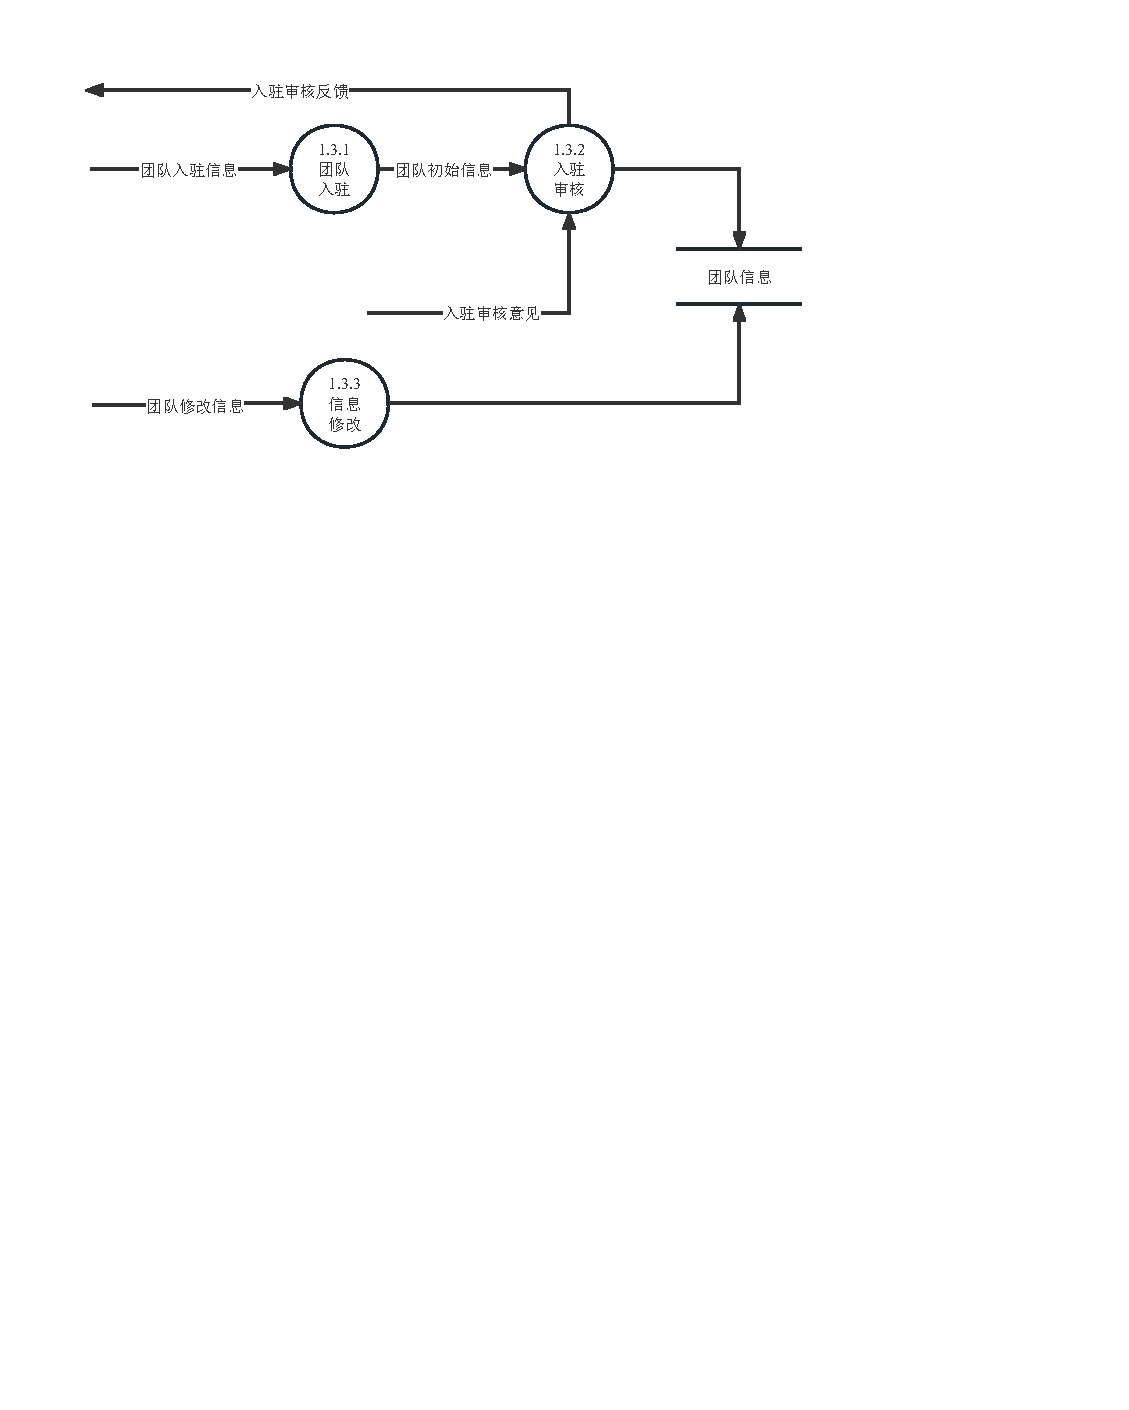
\includegraphics[width=0.95\textwidth]  {fig/信息管理/I_2-3.pdf}} 
    \bicaption{信息管理系统2层数据流图}{Data Flow Diagram for Level 2 of Information Management System}
    \label{0level_data}
    \end{figure}

(1)数据加工词条描述说明
\begin{table}[H]  
\caption{“团队入驻”加工词条描述}  
\begin{center}  
    \begin{tabular}{l p{11cm}} 
        \hline
        \quad 名称:  &   团队入驻 \\
        \hline
        \quad 编号:  & 1.3.1 \\
        \hline
        \quad 简述:  & 生成供审核的用户初始信息 \\
        \hline
        \quad 输入:  & 团队入驻信息 \\
        \hline
        \quad 输出:  & 团队初始信息\\
        \hline
        \quad 逻辑:  & 根据团队填写的入驻信息生成团队初始信息。 \\
        \hline
    \end{tabular}
    \label{tab1}
\end{center}
\end{table}

\begin{algorithm}[H]
    \renewcommand{\thealgorithm}{}
    \caption{“团队入驻”加工小说明} 
    \label{alg3} 
    \begin{algorithmic}[1]
        \STATE Create 团队ID
        \STATE Write 团队入驻信息 + 团队ID To 团队初始信息
    \end{algorithmic} 
\end{algorithm}

\begin{table}[H]  
\caption{“入驻审核”加工词条描述}  
\begin{center}  
    \begin{tabular}{l p{11cm}} 
        \hline
        \quad 名称:  &   入驻审核 \\
        \hline
        \quad 编号:  & 1.3.2 \\
        \hline
        \quad 简述:  & 系统管理员审核团队入驻的功能 \\
        \hline
        \quad 输入:  & 团队初始信息 \\
        \hline
        \quad 输出:  & 入驻审核反馈、团队信息 \\
        \hline
        \quad 逻辑:  & 系统管理员审核团队信息,并给出审核反馈。 \\
        \hline
    \end{tabular}
    \label{tab1}
\end{center}
\end{table}

\begin{algorithm}[H]
    \renewcommand{\thealgorithm}{}
    \caption{“入驻审核”加工小说明} 
    \label{alg3} 
    \begin{algorithmic}[1]
        \IF{Pass Check 团队初始信息} 
        \STATE Write 团队初始信息 To 团队信息
        \STATE Write 入驻审核反馈字段  To 入驻审核反馈
        \ELSE
        \STATE Write 入驻审核反馈字段 To 入驻审核反馈 
        \ENDIF 
    \end{algorithmic} 
\end{algorithm}

\begin{table}[H]  
\caption{“信息修改”加工词条描述}  
\begin{center}  
    \begin{tabular}{l p{11cm}} 
        \hline
        \quad 名称:  &   信息修改 \\
        \hline
        \quad 编号:  & 1.3.3 \\
        \hline
        \quad 简述:  & 修改团队信息的功能 \\
        \hline
        \quad 输入:  & 团队修改信息\\
        \hline
        \quad 输出:  & 团队信息\\
        \hline
        \quad 逻辑:  & 根据团队修改信息修改团队信息。 \\
        \hline
    \end{tabular}
    \label{tab1}
\end{center}
\end{table}

\begin{algorithm}[H] 
    \renewcommand{\thealgorithm}{}
    \caption{“信息修改”加工小说明} 
    \label{alg3} 
    \begin{algorithmic}[1]
        \STATE Update 团队修改信息 In 团队信息 Match 团队ID
    \end{algorithmic} 
\end{algorithm}

(2)数据流词条描述说明
\begin{table}[H]  
\caption{``团队入驻信息"数据流词条描述}  
\begin{center}  
    \begin{tabular}{l p{11cm}} 
        \hline
        \quad 名称:  &  团队入驻信息 \\
        \hline
        \quad 简述:  & 团队为注册输入信息 \\
        \hline
        \quad 来源:  & 源点``志愿团队"\\
        \hline
        \quad 去向:  & 加工``团队入驻" \\
        \hline
        \quad 组成:  & 团队名+电子邮箱+电话号码+团队地址+团队网站 \\
        \hline
    \end{tabular}
    \label{tab1}
\end{center}
\end{table}

\begin{table}[H]  
\caption{``团队初始信息"数据流词条描述}  
\begin{center}  
    \begin{tabular}{l p{11cm}} 
        \hline
        \quad 名称:  &   团队初始信息 \\
        \hline
        \quad 简述:  & 初始的团队信心 \\
        \hline
        \quad 来源:  & 加工``团队入驻"\\
        \hline
        \quad 去向:  & 加工``入驻审核" \\
        \hline
        \quad 组成:  & 团队ID+团队名+电子邮箱+电话号码+团队地址+团队网站\\
        \hline
    \end{tabular}
    \label{tab1}
\end{center}
\end{table}

\begin{table}[H]  
\caption{``入驻审核反馈"数据流词条描述}  
\begin{center}  
    \begin{tabular}{l p{11cm}} 
        \hline
        \quad 名称:  &   入驻审核反馈 \\
        \hline
        \quad 简述:  & 对于入驻审核意见的反馈 \\
        \hline
        \quad 来源:  & 加工``入驻审核" \\
        \hline
        \quad 去向:  & 源点``志愿团队" \\
        \hline
        \quad 组成:  & 入驻审核反馈字段\\
        \hline
    \end{tabular}
    \label{tab1}
\end{center}
\end{table}

\begin{table}[H]  
\caption{``团队修改信息"数据流词条描述}  
\begin{center}  
    \begin{tabular}{l p{11cm}} 
        \hline
        \quad 名称:  &   团队修改信息 \\
        \hline
        \quad 简述:  & 对于团队信息的修改 \\
        \hline
        \quad 来源:  & 源点``志愿团队" \\
        \hline
        \quad 去向:  & 加工``信息修改" \\
        \hline
        \quad 组成:  & 团队ID +电子邮箱+电话号码+团队地址+团队网站+团队名单\\
        \hline
    \end{tabular}
    \label{tab1}
\end{center}
\end{table}

(3)文件词条描述
\begin{table}[H]  
\caption{“团队信息”文件词条描述}  
\begin{center}  
    \begin{tabular}{l p{10cm}} 
        \hline
        \quad 名称:  &   团队信息 \\
        \hline
        \quad 简述:  & 存储团队信息内容\\
        \hline
        \quad 组成:  & 团队ID+团队名+电子邮箱+电话号码+团队地址+团队网站+团队人数+团队名单 \\
        \hline
        \quad 存储方式:  & 以团队ID为关键字。 \\
        \hline
    \end{tabular}
    \label{tab1}
\end{center}
\end{table}

\begin{algorithm}[H] 
    \renewcommand{\thealgorithm}{}
    \caption{“信息修改”加工小说明} 
    \label{alg3} 
    \begin{algorithmic}[1]
        \STATE Update 团队修改信息 In 团队信息 Match 团队ID
    \end{algorithmic} 
\end{algorithm}


\paragraph{用户管理}~{}
\\


\begin{figure}[H]
    \center{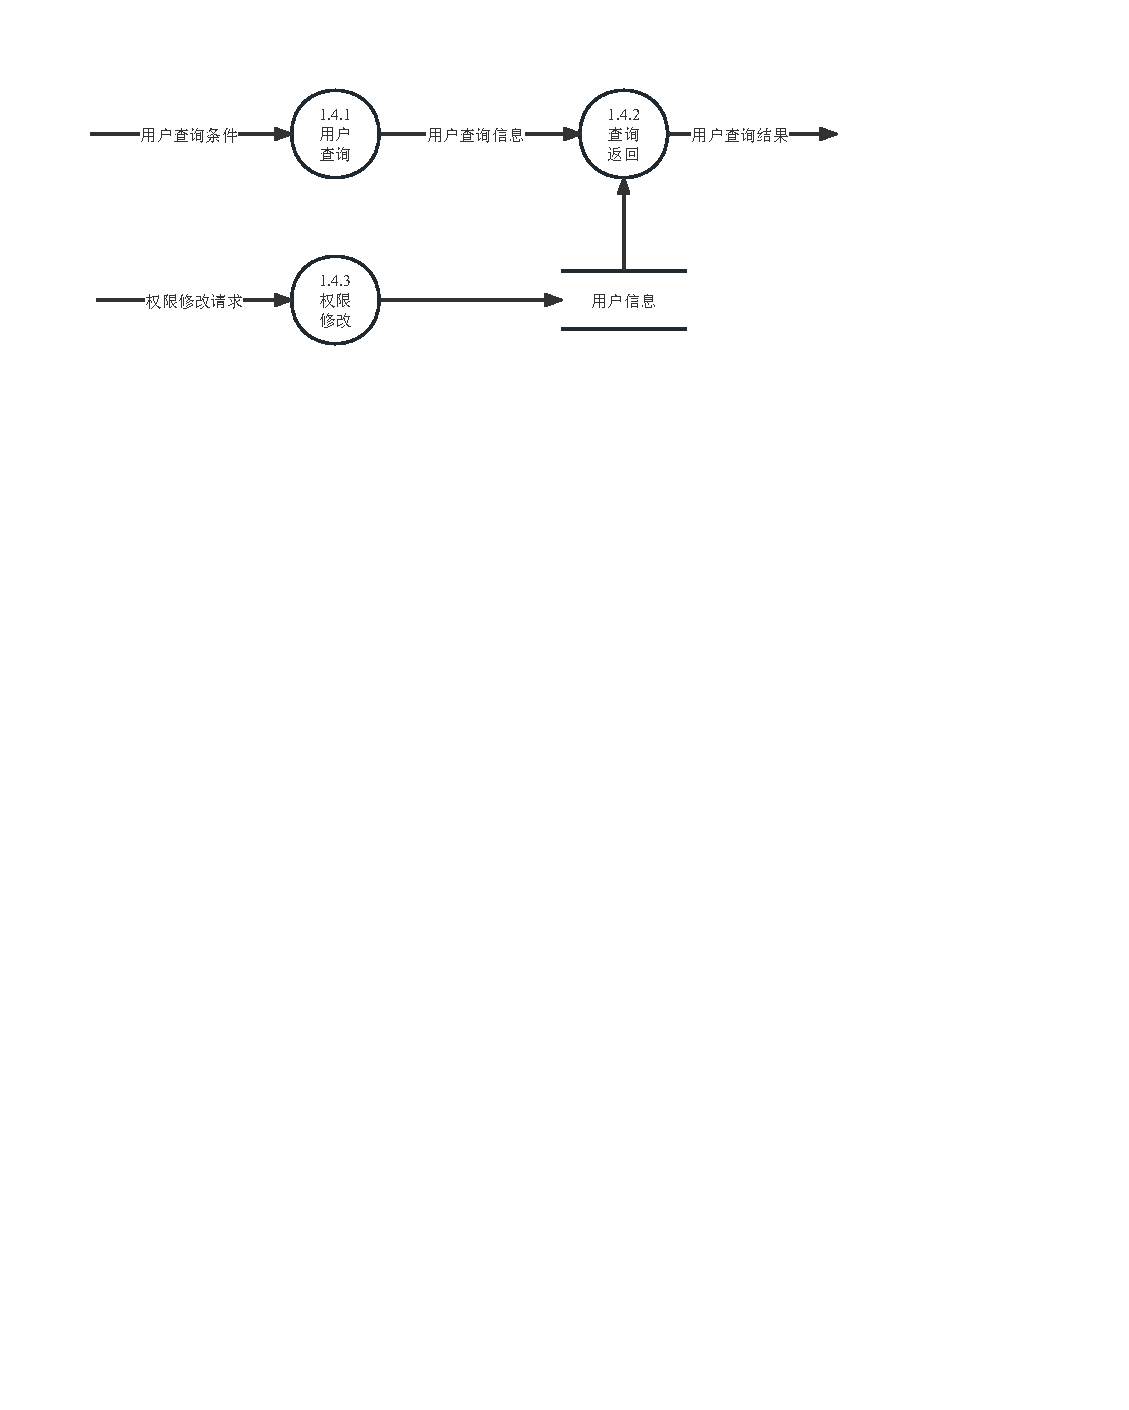
\includegraphics[width=0.95\textwidth]  {fig/信息管理/I_2-4.pdf}} 
    \bicaption{信息管理系统2层数据流图}{Data Flow Diagram for Level 2 of Information Management System}
    \label{0level_data}
    \end{figure}
    
(1)数据加工词条描述说明
\begin{table}[H]  
\caption{“用户查询”加工词条描述}  
\begin{center}  
    \begin{tabular}{l p{11cm}} 
        \hline
        \quad 名称:  &   用户查询 \\
        \hline
        \quad 编号:  & 1.4.1 \\
        \hline
        \quad 简述:  & 查询符合条件的用户 \\
        \hline
        \quad 输入:  & 查询条件 \\
        \hline
        \quad 输出:  & 查询信息\\
        \hline
        \quad 逻辑:  & 根据查询条件生成完整的查询信息。 \\
        \hline
    \end{tabular}
    \label{tab1}
\end{center}
\end{table}

\begin{algorithm}[H] 
    \renewcommand{\thealgorithm}{}
    \caption{“用户查询”加工小说明} 
    \label{alg3} 
    \begin{algorithmic}[1]
        \STATE Get 系统时间 As 查询时间
        \STATE Write 用户查询条件 + 查询时间 To 用户查询信息 
    \end{algorithmic} 
\end{algorithm}

\begin{table}[H]  
\caption{“查询返回”加工词条描述}  
\begin{center}  
    \begin{tabular}{l p{11cm}} 
        \hline
        \quad 名称:  &   查询返回 \\
        \hline
        \quad 编号:  & 1.4.2 \\
        \hline
        \quad 简述:  & 返回符合条件的用户信息 \\
        \hline
        \quad 输入:  & 查询信息、用户信息 \\
        \hline
        \quad 输出:  & 查询结果\\
        \hline
        \quad 逻辑:  & 返回符合查询条件的用户信息作为查询结果。 \\
        \hline
    \end{tabular}
    \label{tab1}
\end{center}
\end{table}

\begin{algorithm}[H] 
    \renewcommand{\thealgorithm}{}
    \caption{“查询返回”加工小说明} 
    \label{alg3} 
    \begin{algorithmic}[1]
        \STATE Select Items In 用户信息 Match 用户查询信息
        \STATE Write Selected Items As 用户查询结果
    \end{algorithmic} 
\end{algorithm}

\begin{table}[H]  
\caption{“权限修改”加工词条描述}  
\begin{center}  
    \begin{tabular}{l p{11cm}} 
        \hline
        \quad 名称:  &   权限修改 \\
        \hline
        \quad 编号:  & 1.4.3 \\
        \hline
        \quad 简述:  & 修改用户的权限 \\
        \hline
        \quad 输入:  & 权限修改请求 \\
        \hline
        \quad 输出:  & 用户信息 \\
        \hline
        \quad 逻辑:  & 系统管理员根据查询到的权限信息设置修改用户相应的权限信息。 \\
        \hline
    \end{tabular}
    \label{tab1}
\end{center}
\end{table}


(2)数据流词条描述说明
\begin{table}[H]  
\caption{``用户查询条件"数据流词条描述}  
\begin{center}  
    \begin{tabular}{l p{11cm}} 
        \hline
        \quad 名称:  &   用户查询条件 \\
        \hline
        \quad 简述:  & 系统管理员对用户信息查询的条件 \\
        \hline
        \quad 来源:  & 源点``系统管理员" \\
        \hline
        \quad 去向:  & 加工``用户查询" \\
        \hline
        \quad 组成:  & 查询关键字 \\
        \hline
    \end{tabular}
    \label{tab1}
\end{center}
\end{table}

\begin{table}[H]  
\caption{``用户查询信息"数据流词条描述}  
\begin{center}  
    \begin{tabular}{l p{11cm}} 
        \hline
        \quad 名称:  &   用户查询信息 \\
        \hline
        \quad 简述:  & 用户信息查询的信息 \\
        \hline
        \quad 来源:  & 加工``用户查询" \\
        \hline
        \quad 去向:  & 加工``查询返回"\\
        \hline
        \quad 组成:  & 查询关键字+查询时间 \\
        \hline
    \end{tabular}
    \label{tab1}
\end{center}
\end{table}

\begin{table}[H]  
\caption{``用户查询结果"数据流词条描述}  
\begin{center}  
    \begin{tabular}{l p{11cm}} 
        \hline
        \quad 名称:  &   用户查询结果 \\
        \hline
        \quad 简述:  & 信息查询的结果 \\
        \hline
        \quad 来源:  & 加工``查询返回" \\
        \hline
        \quad 去向:  & 源点``系统管理员" \\
        \hline
        \quad 组成:  & 用户ID+用户名+账号+密码+用户权限+所属团队+注册时间 \\
        \hline
    \end{tabular}
    \label{tab1}
\end{center}
\end{table}

\begin{table}[H]  
\caption{``权限修改请求"数据流词条描述}  
\begin{center}  
    \begin{tabular}{l p{11cm}} 
        \hline
        \quad 名称:  &   权限修改请求 \\
        \hline
        \quad 简述:  & 对指定用户进行权限修改的请求 \\
        \hline
        \quad 来源:  & 源点``系统管理员"\\
        \hline
        \quad 去向:  & 加工``权限修改" \\
        \hline
        \quad 组成:  & 用户ID+用户权限\\
        \hline
    \end{tabular}
    \label{tab1}
\end{center}
\end{table}




(3)文件词条描述
\begin{table}[H]  
\caption{“用户信息”文件词条描述}  
\begin{center}  
    \begin{tabular}{l p{10cm}} 
        \hline
        \quad 名称:  &   用户信息 \\
        \hline
        \quad 简述:  & 存储用户信息内容\\
        \hline
        \quad 组成:  & 用户ID+用户名+账号+密码+用户权限+所属团队+注册时间 \\
        \hline
        \quad 存储方式:  & 以用户ID为关键字。 \\
        \hline
    \end{tabular}
    \label{tab1}
\end{center}
\end{table}



\paragraph{组队管理}~{}
\\

\begin{figure}[H]
    \center{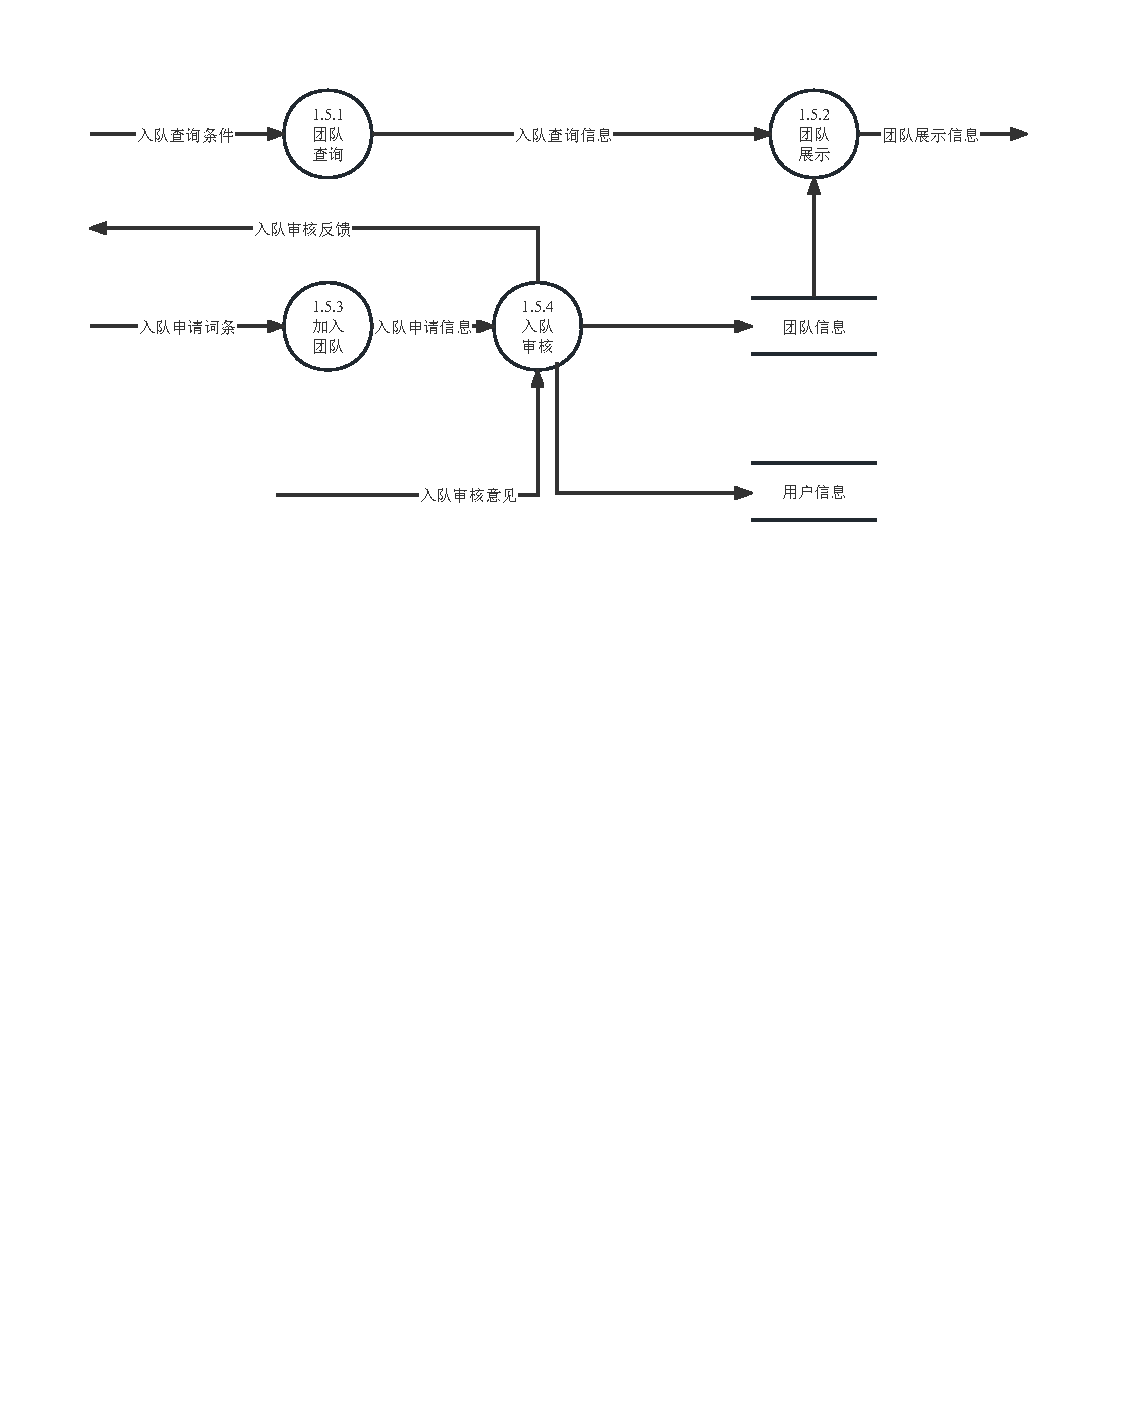
\includegraphics[width=0.95\textwidth]  {fig/信息管理/I_2-5.pdf}} 
    \bicaption{信息管理系统2层数据流图}{Data Flow Diagram for Level 2 of Information Management System}
    \label{0level_data}
    \end{figure}
    
(1)数据加工词条描述说明
\begin{table}[H]  
\caption{“团队查询”加工词条描述}  
\begin{center}  
    \begin{tabular}{l p{11cm}} 
        \hline
        \quad 名称:  &  团队查询 \\
        \hline
        \quad 编号:  & 1.5.1 \\
        \hline
        \quad 简述:  & 查询符合条件的团队的功能 \\
        \hline
        \quad 输入:  & 入队查询条件 \\
        \hline
        \quad 输出:  & 入队查询信息\\
        \hline
        \quad 逻辑:  & 根据查询条件生成完整的查询信息。 \\
        \hline
    \end{tabular}
    \label{tab1}
\end{center}
\end{table}

\begin{algorithm}[H] 
    \renewcommand{\thealgorithm}{}
    \caption{“团队查询”加工小说明} 
    \label{alg3} 
    \begin{algorithmic}[1]
        \STATE Get 系统时间 As 查询时间
        \STATE Write 入队查询条件 + 查询时间 To 入队查询信息 
    \end{algorithmic} 
\end{algorithm}


\begin{table}[H]  
\caption{“团队展示”加工词条描述}  
\begin{center}  
    \begin{tabular}{l p{11cm}} 
        \hline
        \quad 名称:  &   团队展示 \\
        \hline
        \quad 编号:  & 1.5.2 \\
        \hline
        \quad 简述:  & 展示符合条件的团队的功能 \\
        \hline
        \quad 输入:  & 查询信息、团队信息 \\
        \hline
        \quad 输出:  & 团队展示信息\\
        \hline
        \quad 逻辑:  & 根据查询信息、团队信息生成复合条件的团队的团队展示信息。 \\
        \hline
    \end{tabular}
    \label{tab1}
\end{center}
\end{table}

\begin{algorithm}[H] 
    \renewcommand{\thealgorithm}{}
    \caption{“团队展示”加工小说明} 
    \label{alg3} 
    \begin{algorithmic}[1]
        \STATE Select Items In 团队信息 Match 入队查询信息
        \STATE Write Selected Items As 团队展示信息
    \end{algorithmic} 
\end{algorithm}


\begin{table}[H]  
\caption{“加入团队”加工词条描述}  
\begin{center}  
    \begin{tabular}{l p{11cm}} 
        \hline
        \quad 名称:  &   加入团队 \\
        \hline
        \quad 编号:  & 1.5.3 \\
        \hline
        \quad 简述:  & 用户加入团队的功能 \\
        \hline
        \quad 输入:  & 入队申请词条 \\
        \hline
        \quad 输出:  & 入队申请信息 \\
        \hline
        \quad 逻辑:  & 根据查询到的团队信息填写生产入队申请。 \\
        \hline
    \end{tabular}
    \label{tab1}
\end{center}
\end{table}

\begin{algorithm}[H]
    \renewcommand{\thealgorithm}{}
    \caption{“加入团队”加工小说明} 
    \label{alg3} 
    \begin{algorithmic}[1]
        \STATE Get 系统时间 As 申请时间
        \STATE Select Items In 用户信息 Match 用户ID
        \STATE Get 用户ID + 用户名 + 申请时间 From Selected Items
        \STATE Write 入队申请词条 +用户ID +用户名 + 所属团队 + 申请时间 To 入队申请信息
    \end{algorithmic} 
\end{algorithm}


\begin{table}[H]  
\caption{“入队审核”加工词条描述}  
\begin{center}  
    \begin{tabular}{l p{11cm}} 
        \hline
        \quad 名称:  &   入驻审核 \\
        \hline
        \quad 编号:  & 1.5.4 \\
        \hline
        \quad 简述:  & 志愿团队审核用户入队的功能 \\
        \hline
        \quad 输入:  & 入队申请信息、入队审核信息 \\
        \hline
        \quad 输出:  & 入队审核反馈、团队信息、用户信息 \\
        \hline
        \quad 逻辑:  & 志愿团队审核入队用户信息,作出决定后更新团队信息和用户信息,并给出审核反馈。 \\
        \hline
    \end{tabular}
    \label{tab1}
\end{center}
\end{table}

\begin{algorithm}[H]
    \renewcommand{\thealgorithm}{}
    \caption{“入队审核”加工小说明} 
    \label{alg3} 
    \begin{algorithmic}[1]
        \IF{Pass Check 入队申请信息} 
        \STATE Update Item.所属团队 In 用户信息 Match 用户ID From 入队申请信息
        \STATE Update Item In 团队信息 Match 团队ID From 入队申请信息
        \STATE Write 入队审核意见  To 入队审核反馈
        \ELSE
        \STATE Write 入队审核意见  To 入队审核反馈 
        \ENDIF 
    \end{algorithmic} 
\end{algorithm}


(2)数据流词条描述说明
\begin{table}[H]  
\caption{``入队查询条件"数据流词条描述}  
\begin{center}  
    \begin{tabular}{l p{11cm}} 
        \hline
        \quad 名称:  &   入队查询条件 \\
        \hline
        \quad 简述:  & 对团队查询的条件 \\
        \hline
        \quad 来源:  & 源点``系统管理员" \\
        \hline
        \quad 去向:  & 加工``团队查询" \\
        \hline
        \quad 组成:  & 查询关键字 \\
        \hline
    \end{tabular}
    \label{tab1}
\end{center}
\end{table}

\begin{table}[H]  
\caption{``入队查询信息"数据流词条描述}  
\begin{center}  
    \begin{tabular}{l p{11cm}} 
        \hline
        \quad 名称:  &   入队查询信息 \\
        \hline
        \quad 简述:  & 团队查询的信息 \\
        \hline
        \quad 来源:  & 源点``团队查询" \\
        \hline
        \quad 去向:  & 加工``团队展示" \\
        \hline
        \quad 组成:  & 查询关键字+查询时间 \\
        \hline
    \end{tabular}
    \label{tab1}
\end{center}
\end{table}

\begin{table}[H]  
\caption{``团队展示信息"数据流词条描述}  
\begin{center}  
    \begin{tabular}{l p{11cm}} 
        \hline
        \quad 名称:  &   团队展示信息 \\
        \hline
        \quad 简述:  & 团队查询的结果 \\
        \hline
        \quad 来源:  & 加工``团队展示" \\
        \hline
        \quad 去向:  & 源点``志愿者" \\
        \hline
        \quad 组成:  & 团队名+团队人数+团队名单 \\
        \hline
    \end{tabular}
    \label{tab1}
\end{center}
\end{table}

\begin{table}[H]  
\caption{``入队申请词条"数据流词条描述}  
\begin{center}  
    \begin{tabular}{l p{11cm}} 
        \hline
        \quad 名称:  &   入队申请词条 \\
        \hline
        \quad 简述:  & 用户加入团队的申请 \\
        \hline
        \quad 来源:  & 源点``志愿者"\\
        \hline
        \quad 去向:  & 加工``加入团队" \\
        \hline
        \quad 组成:  & 入队申请说明字段 +用户ID+团队ID\\
        \hline
    \end{tabular}
    \label{tab1}
\end{center}
\end{table}

\begin{table}[H]  
\caption{``入队申请信息"数据流词条描述}  
\begin{center}  
    \begin{tabular}{l p{11cm}} 
        \hline
        \quad 名称:  &   入队申请信息 \\
        \hline
        \quad 简述:  & 完整的加入团队的申请 \\
        \hline
        \quad 来源:  & 加工``加入团队"\\
        \hline
        \quad 去向:  & 加工``入队审核" \\
        \hline
        \quad 组成:  & 入队申请说明字段+用户ID+用户名+所属团队+申请时间\\
        \hline
    \end{tabular}
    \label{tab1}
\end{center}
\end{table}


\begin{table}[H]  
\caption{``入队审核反馈"数据流词条描述}  
\begin{center}  
    \begin{tabular}{l p{11cm}} 
        \hline
        \quad 名称:  &   入队审核反馈 \\
        \hline
        \quad 简述:  & 对于入队审核意见的反馈 \\
        \hline
        \quad 来源:  & 加工``入驻审核" \\
        \hline
        \quad 去向:  & 源点``志愿者" \\
        \hline
        \quad 组成:  & 入队审核反馈字段\\
        \hline
    \end{tabular}
    \label{tab1}
\end{center}
\end{table}

(3)文件词条描述
\begin{table}[H]  
\caption{“用户信息”文件词条描述}  
\begin{center}  
    \begin{tabular}{l p{10cm}} 
        \hline
        \quad 名称:  &   用户信息 \\
        \hline
        \quad 简述:  & 存储用户信息内容\\
        \hline
        \quad 组成:  & 用户ID+用户名+账号+密码+用户权限+所属团队+注册时间 \\
        \hline
        \quad 存储方式:  & 以用户ID为关键字。 \\
        \hline
    \end{tabular}
    \label{tab1}
\end{center}
\end{table}


\begin{table}[H]  
\caption{“团队信息”文件词条描述}  
\begin{center}  
    \begin{tabular}{l p{10cm}} 
        \hline
        \quad 名称:  &   团队信息 \\
        \hline
        \quad 简述:  & 存储团队信息内容\\
        \hline
        \quad 组成:  & 团队ID+团队名+电子邮箱+电话号码+团队地址+团队网站+团队人数+团队名单 \\
        \hline
        \quad 存储方式:  & 以团队ID为关键字。 \\
        \hline
    \end{tabular}
    \label{tab1}
\end{center}
\end{table}


\subsubsection{志愿服务系统}
以下是志愿服务系统的1层数据流图、加工子图以及对应的数据字典和文件。志愿服务系统分为项目发布、项目报名的项目管理。

\begin{figure}[H]
    \center{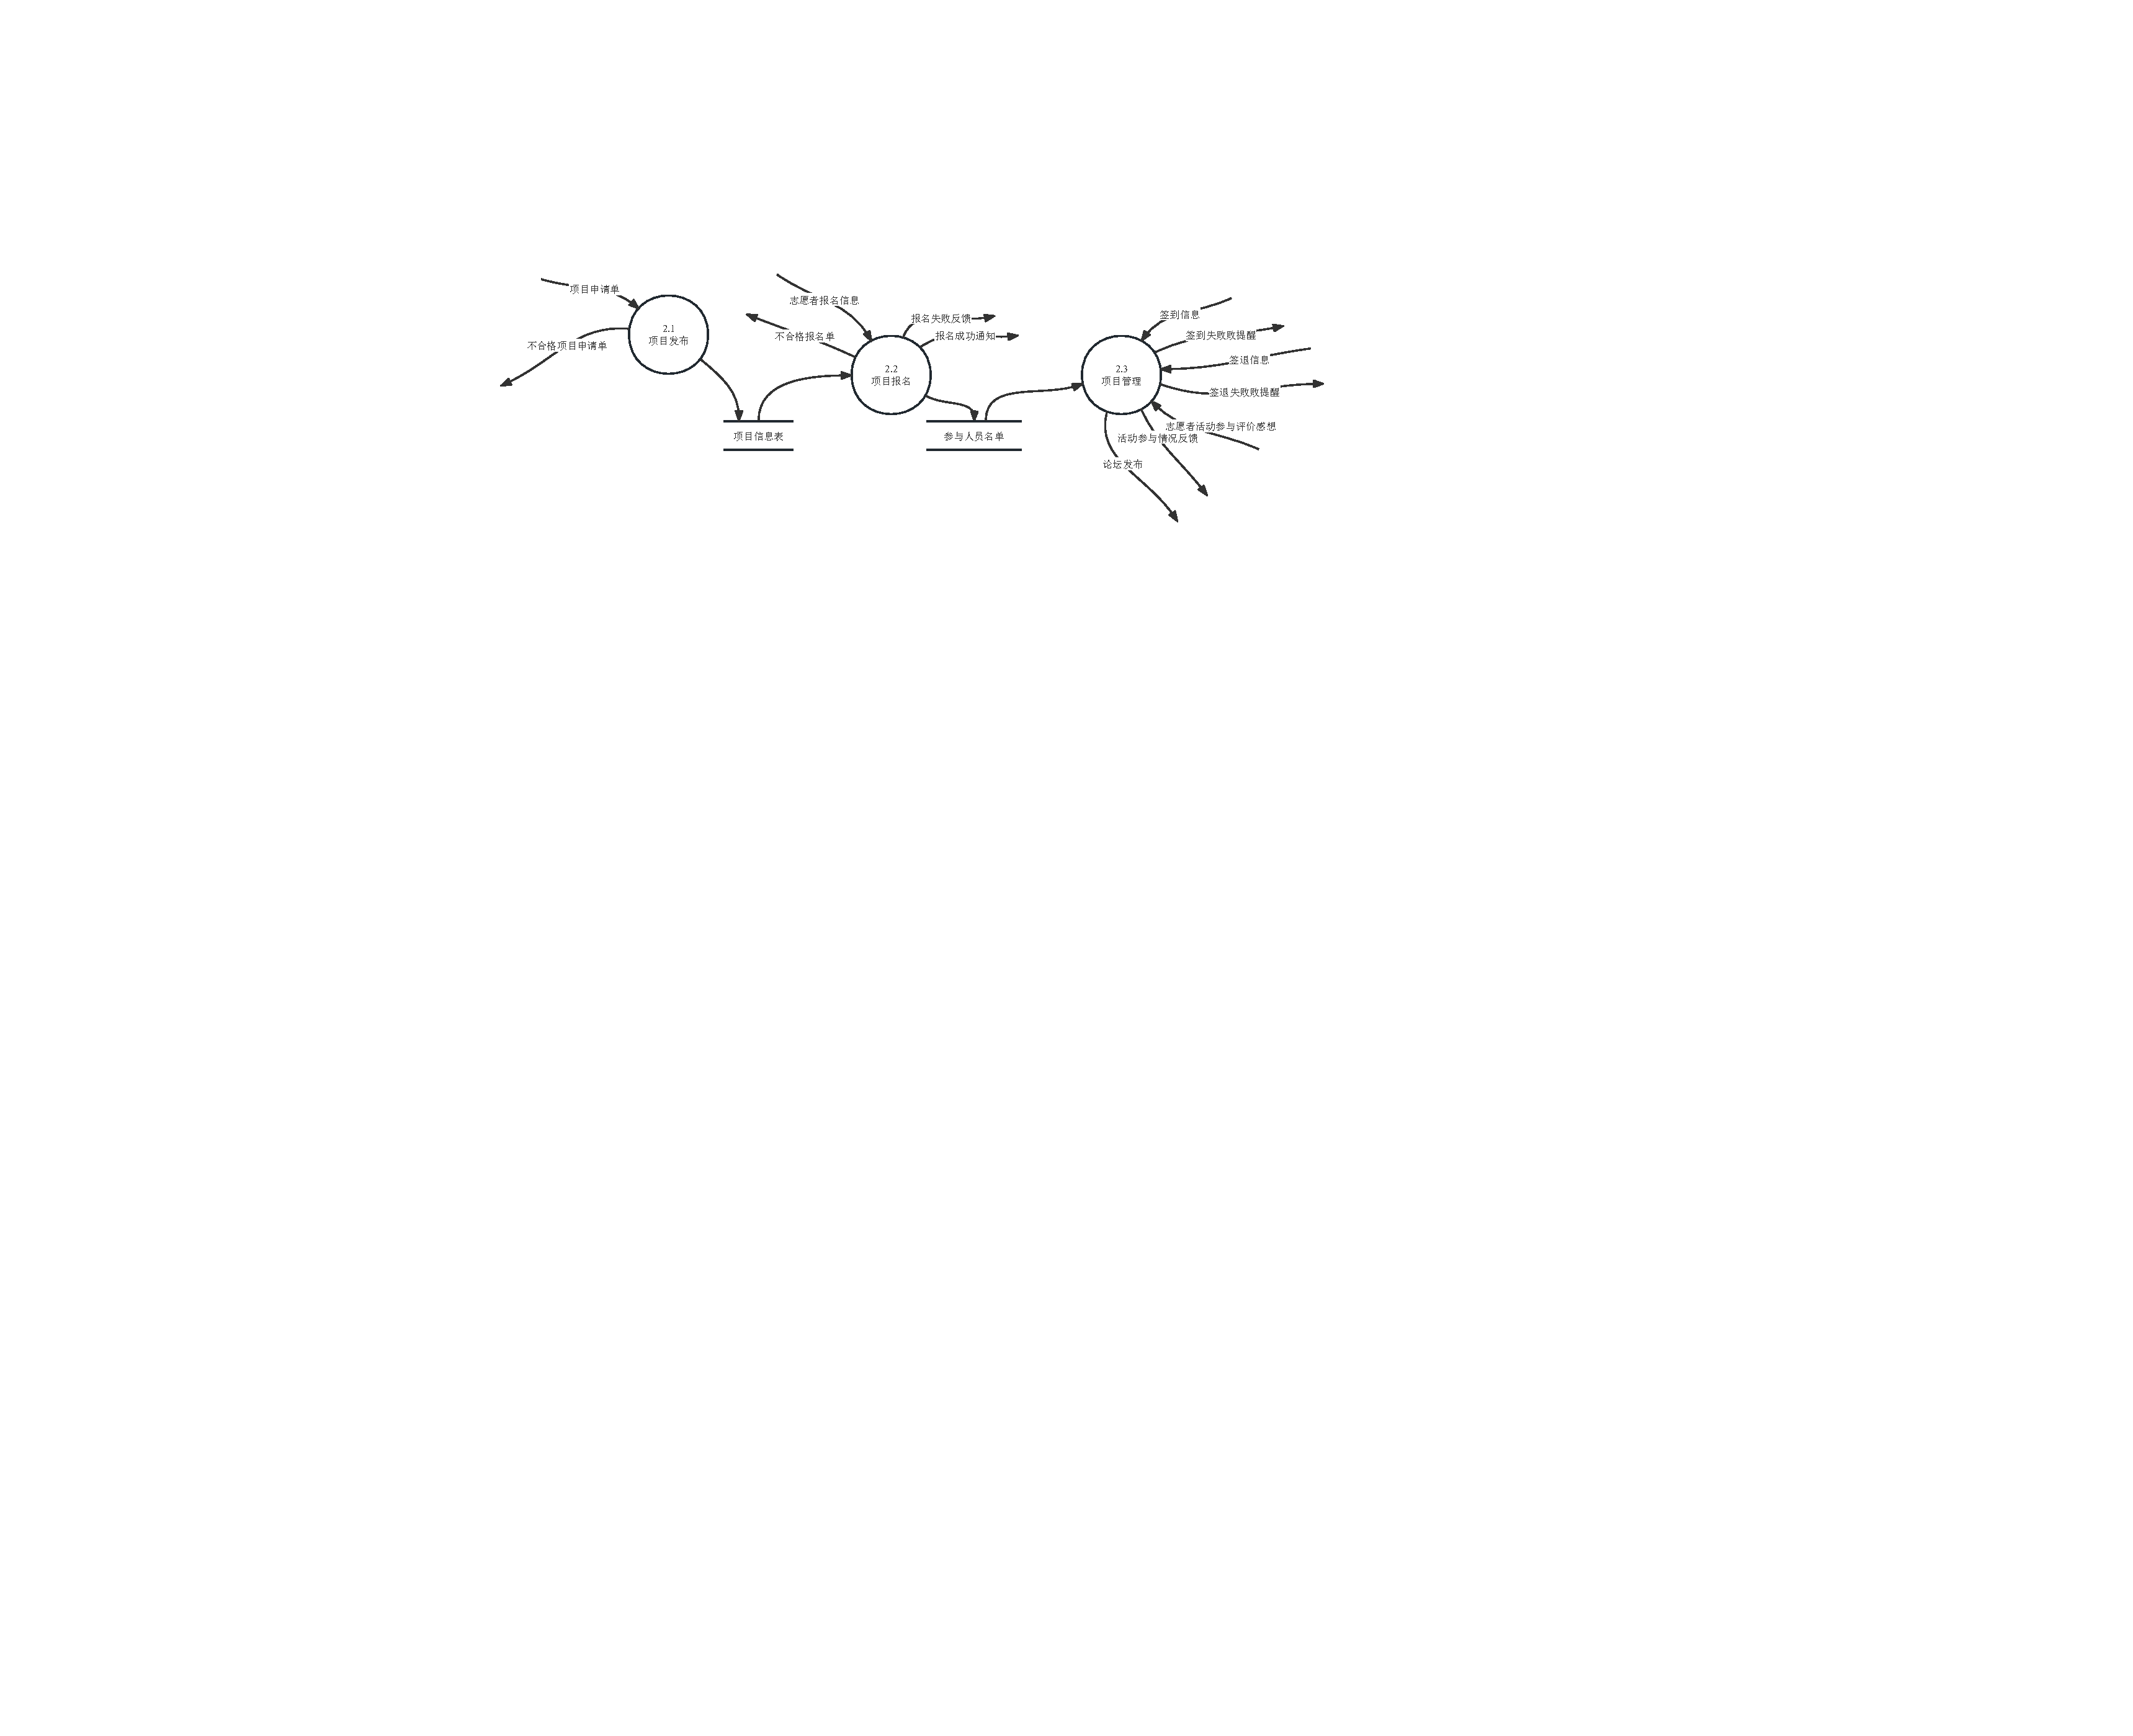
\includegraphics[width=0.95\textwidth]  {fig/志愿服务/V_1.pdf}} 
    \bicaption{志愿服务系统1层数据流图}{Data Flow Diagram for Level 1 of Volunteer Service System}
    \end{figure}

% (1)数据加工词条描述说明

% \begin{table}[H]  
\caption{“志愿项目发布”加工词条描述}  
\begin{center}  
    \begin{tabular}{l p{11cm}} 
        \hline
        \quad 名称: & 志愿项目发布\\
        \hline
        \quad 编号: & 1.1 \\
        \hline
        \quad 简述: & 志愿团队提交志愿项目申请,提交成功后正式在Volunet上展示 \\
        \hline
        \quad 输入:& 项目申请单 \\
        \hline
        \quad 输出:& 项目信息表、不合格项目申请单\\
        \hline
        \quad 逻辑:& 根据志愿团队提交的项目申请单进行审核,审核不通过返回不合格信息提示,审核通过编入项目ID,并发布在Volunet。 \\
        \hline
    \end{tabular}
    \label{tab1}
\end{center}
\end{table}

\begin{table}[H]  
\caption{“项目报名”加工词条描述}  
\begin{center}  
    \begin{tabular}{l p{11cm}} 
        \hline
        \quad 名称: & 项目报名 \\
        \hline
        \quad 编号: & 1.2 \\
        \hline
        \quad 简述: & 项目发布之后,感兴趣的志愿者报名参与该项目。志愿团队根据志愿者报名单选出合适的志愿者,作为最终参与项目志愿者 \\
        \hline
        \quad 输入: & 志愿者报名信息 \\
        \hline
        \quad 输出: & 不合格信息、报名成功反馈、报名失败反馈、参与人员名单\\
        \hline
        \quad 逻辑: & 志愿团队根据志愿者填写的报名单生成参与人员名单。 \\
        \hline
    \end{tabular}
    \label{tab1}
\end{center}
\end{table}

\begin{table}[H]  
\caption{“项目管理”加工词条描述}  
\begin{center}  
    \begin{tabular}{l p{11cm}} 
        \hline
        \quad 名称: & 项目管理 \\
        \hline
        \quad 编号: & 1.3 \\
        \hline
        \quad 简述: & 志愿者在项目进行过程中签到签退,结束后提交反馈,以上信息反馈给志愿团队。 \\
        \hline
        \quad 输入: & 签到信息、签退信息、志愿者反馈 \\
        \hline
        \quad 输出: & 签到失败信息、签退失败信息、活动参与情况反馈、论坛帖子 \\
        \hline
        \quad 逻辑: & 根据志愿者签到信息、签退信息、志愿者反馈生成活动参与情况报告发给志愿团队,并将相应内容生成帖子发布在论坛。 \\
        \hline
    \end{tabular}
    \label{tab1}
\end{center}
\end{table}


% (2)数据流词条描述说明

% 
    
    

    
    
    
   
    
    \begin{table}[H]  
    \caption{``报名失败反馈"数据流词条描述}  
    \begin{center}  
        \begin{tabular}{l p{11cm}} 
            \hline
            \quad 名称: & 报名失败反馈 \\
            \hline
            \quad 简述: & 提供项目报名反馈给未入选志愿者 \\
            \hline
            \quad 来源: & 加工``项目报名" \\
            \hline
            \quad 去向: & 源点``志愿者" \\
            \hline
            \quad 组成: & 项目报名失败信息  \\
            \hline
        \end{tabular}
        \label{tab1}
    \end{center}
    \end{table}

    \begin{table}[H]  
    \caption{``报名成功反馈"数据流词条描述}  
    \begin{center}  
        \begin{tabular}{l p{11cm}} 
            \hline
            \quad 名称: & 报名成功反馈 \\
            \hline
            \quad 简述: & 提供项目报名反馈给入选志愿者 \\
            \hline
            \quad 来源: & 加工``项目报名" \\
            \hline
            \quad 去向: & 源点``志愿者" \\
            \hline
            \quad 组成: & 项目报名成功信息  \\
            \hline
        \end{tabular}
        \label{tab1}
    \end{center}
    \end{table}
    
    \begin{table}[H]  
    \caption{``签到信息"数据流词条描述}  
    \begin{center}  
        \begin{tabular}{l p{11cm}} 
            \hline
            \quad 名称: & 签到信息 \\
            \hline
            \quad 简述: & 志愿者在活动地点打卡签到信息 \\
            \hline
            \quad 来源: & 源点``志愿者" \\
            \hline
            \quad 去向: & 加工``项目管理"\\
            \hline
            \quad 组成: & 志愿者ID+志愿项目ID+签到标记+签到时间+签到地点  \\
            \hline
        \end{tabular}
        \label{tab1}
    \end{center}
    \end{table}

    \begin{table}[H]  
    \caption{``签到失败信息反馈"数据流词条描述}  
    \begin{center}  
        \begin{tabular}{l p{11cm}} 
            \hline
            \quad 名称: & 签到失败信息反馈 \\
            \hline
            \quad 简述: & 志愿者在活动地点打卡签到失败信息反馈 \\
            \hline
            \quad 来源: & 源点``志愿者" \\
            \hline
            \quad 去向: & 加工``项目管理"\\
            \hline
            \quad 组成: & 志愿者ID+志愿项目ID+签到失败原因  \\
            \hline
        \end{tabular}
        \label{tab1}
    \end{center}
    \end{table}

   \begin{table}[H]  
    \caption{``签退信息"数据流词条描述}  
    \begin{center}  
        \begin{tabular}{l p{11cm}} 
            \hline
            \quad 名称: & 签退信息 \\
            \hline
            \quad 简述: & 志愿者在活动地点打卡签退信息 \\
            \hline
            \quad 来源: & 源点``志愿者" \\
            \hline
            \quad 去向: & 加工``项目管理"\\
            \hline
            \quad 组成: & 志愿者ID+志愿项目ID+签退标记+签退时间+签退地点  \\
            \hline
        \end{tabular}
        \label{tab1}
    \end{center}
    \end{table}


    \begin{table}[H]  
    \caption{``签退失败信息反馈"数据流词条描述}  
    \begin{center}  
        \begin{tabular}{l p{11cm}} 
            \hline
            \quad 名称: & 签退失败信息反馈 \\
            \hline
            \quad 简述: & 志愿者在活动地点打卡签退失败信息反馈 \\
            \hline
            \quad 来源: & 源点``志愿者" \\
            \hline
            \quad 去向: & 加工``项目管理"\\
            \hline
            \quad 组成: & 志愿者ID+志愿项目ID+签退失败原因  \\
            \hline
        \end{tabular}
        \label{tab1}
    \end{center}
    \end{table}

    
    \begin{table}[H]  
    \caption{``志愿者参与反馈信息"数据流词条描述}  
    \begin{center}  
        \begin{tabular}{l p{11cm}} 
            \hline
            \quad 名称: & 志愿者参与反馈信息 \\
            \hline
            \quad 简述: & 志愿者参与志愿项目之后提交相应反馈信息 \\
            \hline
            \quad 来源: & 源点``志愿者" \\
            \hline
            \quad 去向: & 加工``项目管理" \\
            \hline
            \quad 组成: & 志愿者ID+志愿项目ID+星级评价+文字反馈+图片\\
            \hline
        \end{tabular}
        \label{tab1}
    \end{center}
    \end{table}


    \begin{table}[H]  
    \caption{``项目参与情况反馈信息"数据流词条描述}  
    \begin{center}  
        \begin{tabular}{l p{11cm}} 
            \hline
            \quad 名称: & 项目参与情况反馈信息 \\
            \hline
            \quad 简述: & 志愿者在该项目参与情况信息反馈给志愿团队 \\
            \hline
            \quad 来源: & 加工``项目管理" \\
            \hline
            \quad 去向: & 源点``志愿团队" \\
            \hline
            \quad 组成: & {志愿者ID+签到信息+签退信息+志愿者评分+文字反馈}\\
            \hline
        \end{tabular}
        \label{tab1}
    \end{center}
    \end{table}
    

% (3)文件词条描述

% 





\paragraph{项目发布}~{}
\\

\begin{figure}[H]
    \center{
\includegraphics[width=0.95\textwidth]  {fig/志愿服务/V_2-1.pdf}} 
    \bicaption{志愿服务系统2层数据流图}{Data Flow Diagram for Level 2 of Volunteer Service System}
    \end{figure}

(1)数据加工词条描述说明

\begin{table}[H]  
\caption{“检查申请单”加工词条描述}  
\begin{center}  
    \begin{tabular}{l p{11cm}} 
        \hline
        \quad 名称: & 检查申请单\\
        \hline
        \quad 编号: & 2.1.1 \\
        \hline
        \quad 简述: & 检查志愿团队所提交志愿项目申请单是否合格 \\
        \hline
        \quad 输入:& 项目申请单 \\
        \hline
        \quad 输出:& 通过审核项目单、不合格项目申请单\\
        \hline
        \quad 逻辑:& 根据志愿团队提交的项目申请单进行审核,审核不通过返回不合格信息提示,审核通过进入下一级加工。 \\
        \hline
    \end{tabular}
    \label{tab1}
\end{center}
\end{table}

\begin{algorithm}[H]
    \renewcommand{\thealgorithm}{}
    \caption{“检查申请单”加工小说明} 
    \label{alg3} 
    \begin{algorithmic}[1]
        \IF{Pass Check 项目申请单 then}
        \STATE Generate 项目审核通过字段 Based on 项目申请单
        \ELSE
        \STATE Generate 不合格原因+{不合格条目+修改建议} Based on 项目申请单
        \STATE Write 不合格原因+{不合格条目+修改建议} to 不合格项目申请单
        \ENDIF 
    \end{algorithmic} 
\end{algorithm}



\begin{table}[H]  
\caption{“项目登记管理”加工词条描述}  
\begin{center}  
    \begin{tabular}{l p{11cm}} 
        \hline
        \quad 名称: & 项目登记管理\\
        \hline
        \quad 编号: & 2.1.2 \\
        \hline
        \quad 简述: & 将审核通过的项目单进行编号登记,并发布到项目中心 \\
        \hline
        \quad 输入:& 通过审核项目单 \\
        \hline
        \quad 输出:& 项目信息表\\
        \hline
        \quad 逻辑:& 根据志愿团队ID和项目申请时间编订该志愿项目的ID编号,并将项目信息存储在项目信息表中。 \\
        \hline
    \end{tabular}
    \label{tab1}
\end{center}
\end{table}


\begin{algorithm}[H]
    \renewcommand{\thealgorithm}{}
    \caption{“项目登记管理”加工小说明} 
    \label{alg3} 
    \begin{algorithmic}[1]
        \IF{项目审核通过字段 is True then}
        \STATE Get 志愿团队ID+当前时间戳 As 志愿项目ID
        \STATE Write 志愿项目ID+志愿团队ID++志愿项目名称+志愿项目简介+开展起止时间+开展地点+\{志愿者种类+志愿者人数+志愿者工作内容\} to 项目信息表
        \ENDIF 
    \end{algorithmic} 
\end{algorithm}

(2)数据流词条描述说明

\begin{table}[H]  
    \caption{``项目申请单"数据流词条描述}  
    \begin{center}  
        \begin{tabular}{l p{11cm}} 
            \hline
            \quad 名称: & 项目申请单 \\
            \hline
            \quad 简述: & 志愿团队申报志愿项目的申请单 \\
            \hline
            \quad 来源: & 源点``志愿团队" \\
            \hline
            \quad 去向: & 加工``项目发布" \\
            \hline
            \quad 组成: & 志愿团队名称+志愿团队ID+志愿项目名称+志愿项目简介+开展起止时间+开展地点+\{志愿者种类+志愿者人数+志愿者工作内容\} \\
            \hline
        \end{tabular}
        \label{tab1}
    \end{center}
    \end{table}


    \begin{table}[H]  
    \caption{``不合格项目申请单"数据流词条描述}  
    \begin{center}  
        \begin{tabular}{l p{11cm}} 
            \hline
            \quad 名称: & 不合格项目申请单 \\
            \hline
            \quad 简述: & 项目申请不合格信息 \\
            \hline
            \quad 来源: & 加工``项目发布" \\
            \hline
            \quad 去向: & 源点``志愿团队" \\
            \hline
            \quad 组成: & 志愿项目名称+不合格原因+{不合格条目+修改建议}  \\
            \hline
        \end{tabular}
        \label{tab1}
    \end{center}
    \end{table}


   \begin{table}[H]  
    \caption{``通过审核项目单"数据流词条描述}  
    \begin{center}  
        \begin{tabular}{l p{11cm}} 
            \hline
            \quad 名称: & 通过审核项目单 \\
            \hline
            \quad 简述: & 项目通过审核之后将项目信息进行登记管理 \\
            \hline
            \quad 来源: & 加工``项目发布" \\
            \hline
            \quad 去向: & 源点``志愿团队" \\
            \hline
            \quad 组成: & 志愿团队名称+志愿团队ID+志愿项目名称+志愿项目简介+开展起止时间+开展地点+\{志愿者种类+志愿者人数+志愿者工作内容\}+项目审核通过字段  \\
            \hline
        \end{tabular}
        \label{tab1}
    \end{center}
    \end{table}

(3)文件词条描述

\begin{table}[H]
  \begin{center}
    \caption{“志愿项目信息表”文件词条描述}
    %\setlength{\tabcolsep}{10mm}{
    \begin{tabular}{l p{10cm}}
      \hline
      名称: &  志愿项目信息表\\
      \hline
      简述:  &  志愿团队申请通过的志愿项目\\
      \hline
      组成:  &  志愿项目名称+志愿项目ID+志愿团队名称+开展起止时间+开展地点+\{志愿者种类+志愿者人数+志愿者工作内容\}\\
      \hline
      存储方式:  &  以志愿项目ID为关键字\\
      \hline
    \end{tabular}
    \label{志愿项目信息表}
  \end{center}
\end{table}


\paragraph{项目报名}~{}
\\

\begin{figure}[H]
    \center{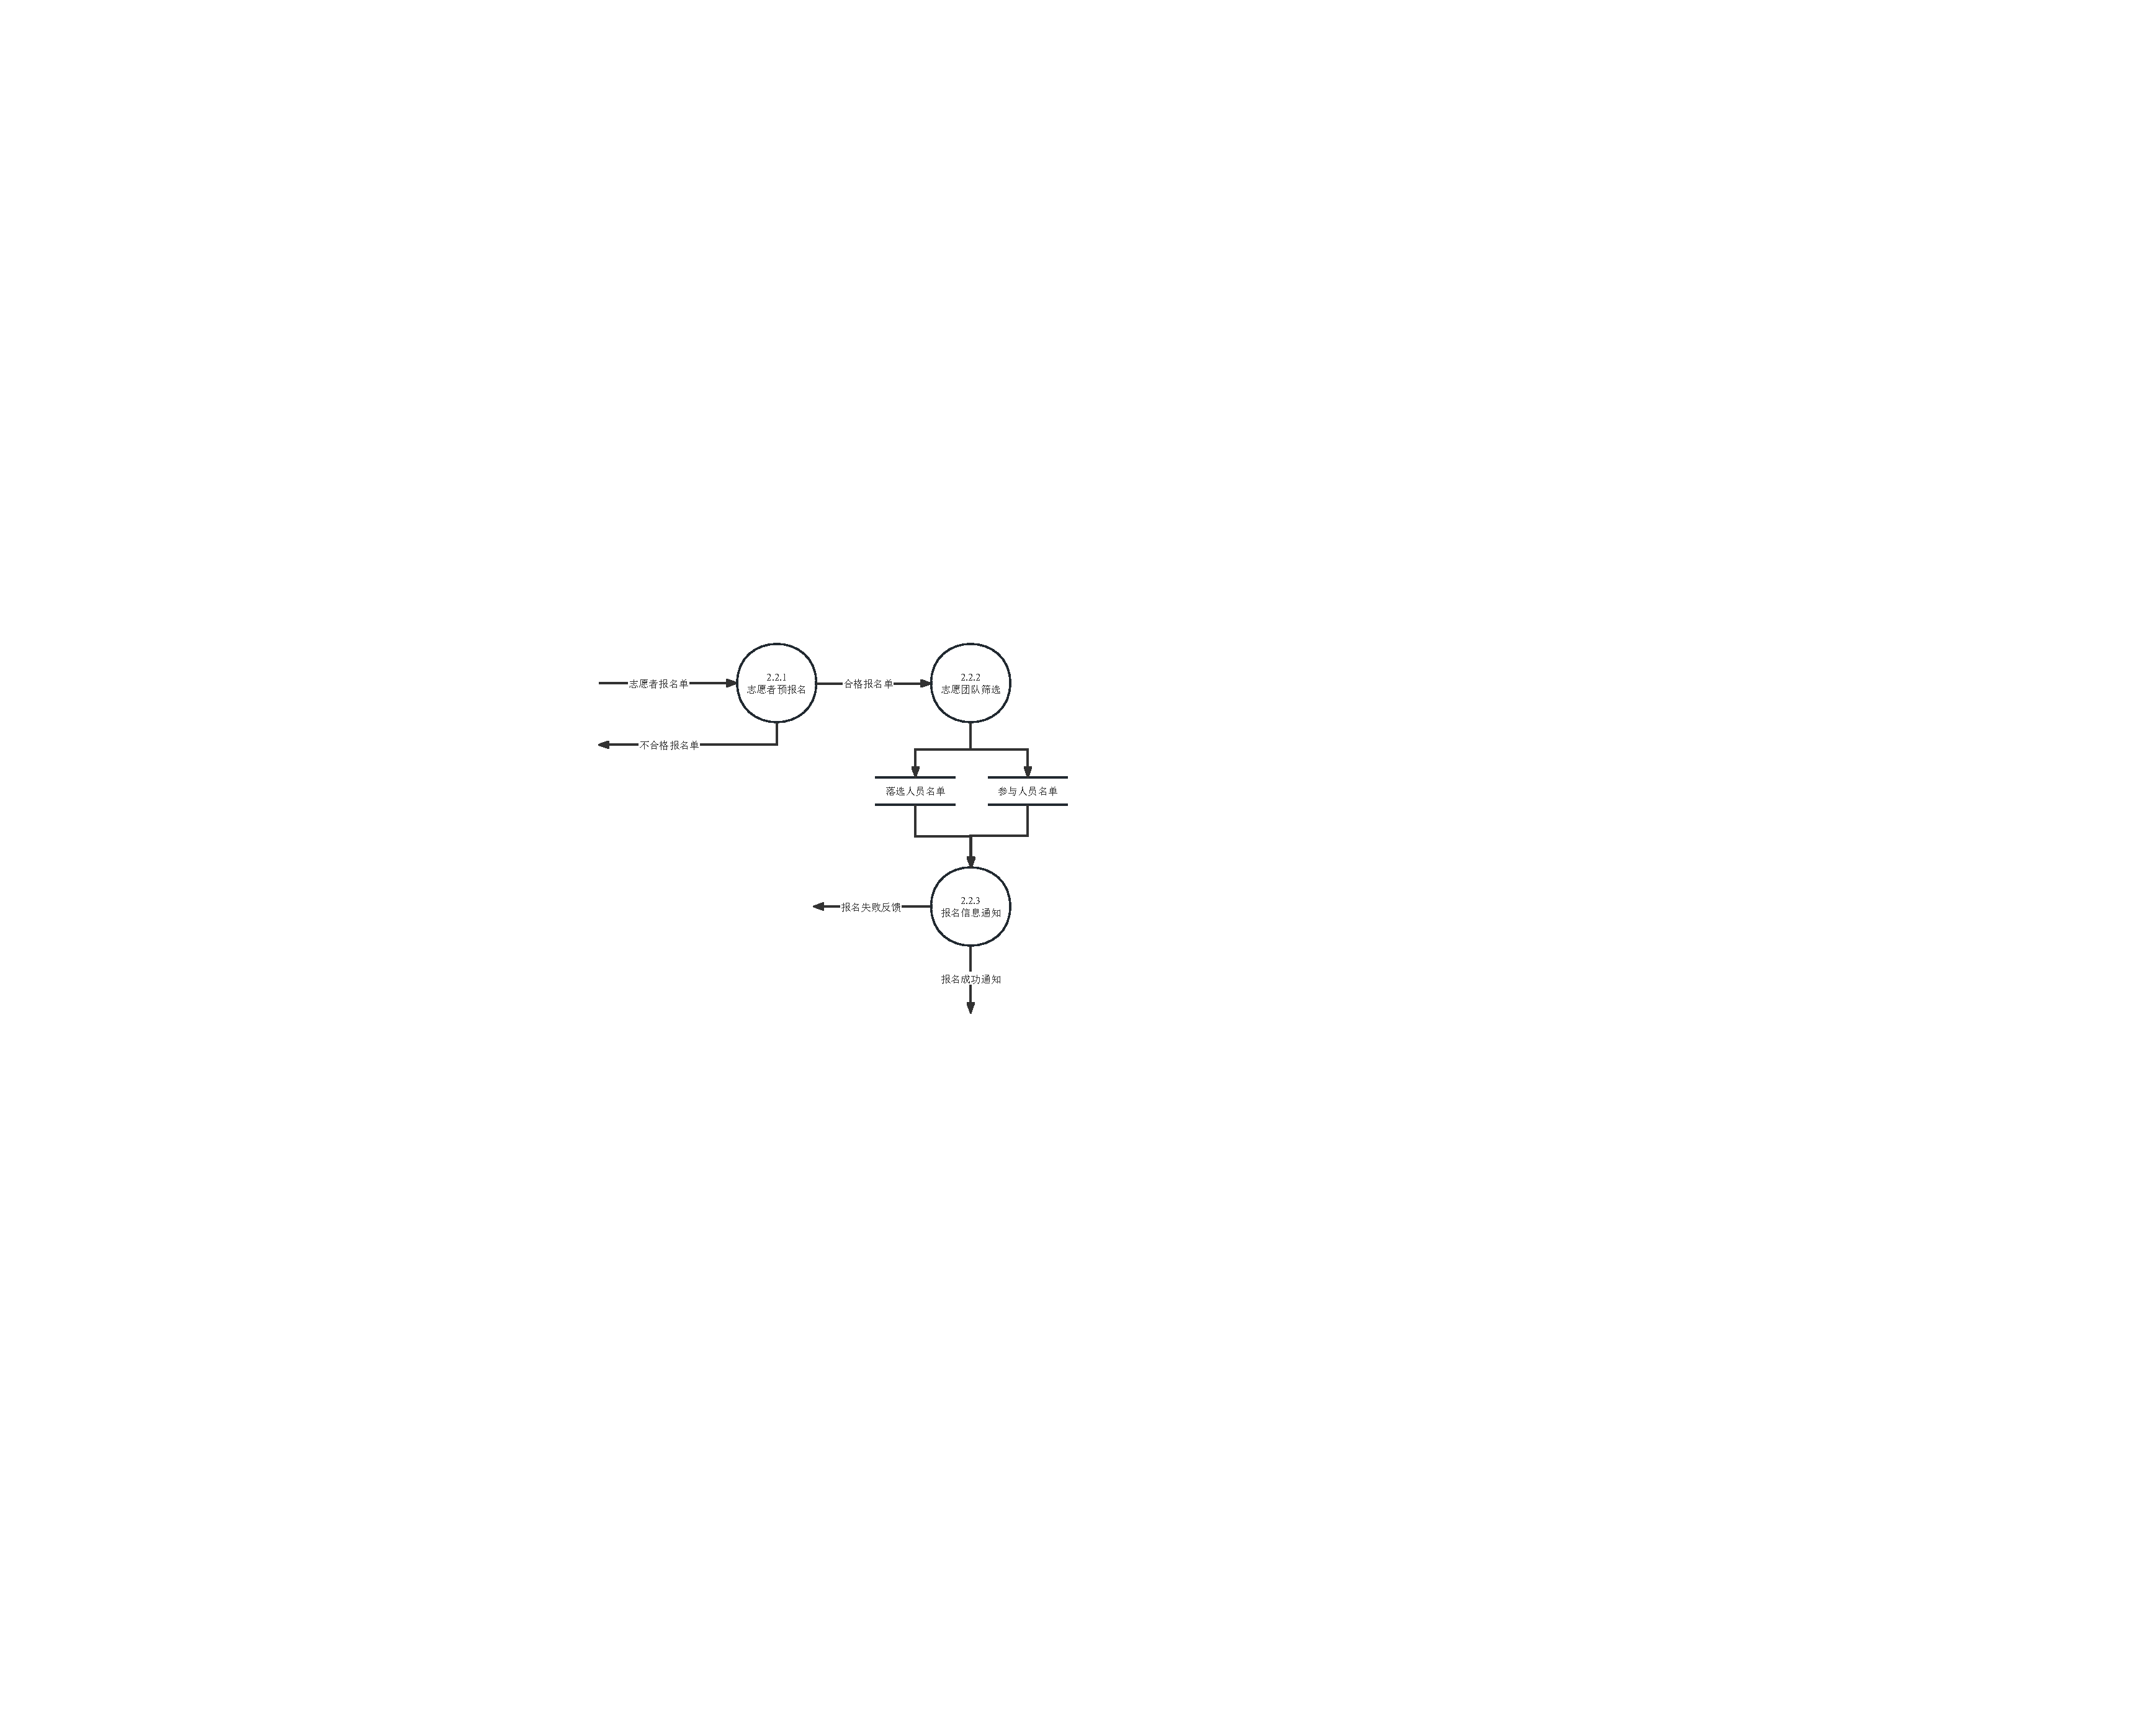
\includegraphics[width=0.95\textwidth]  {fig/志愿服务/V_2-2.2.pdf}} 
    \bicaption{志愿服务系统2层数据流图}{Data Flow Diagram for Level 2 of Volunteer Service System}
    \end{figure}

(1)数据加工词条描述说明

\begin{table}[H]  
\caption{``志愿者预报名”加工词条描述}  
\begin{center}  
    \begin{tabular}{l p{11cm}} 
        \hline
        \quad 名称: & 志愿者预报名\\
        \hline
        \quad 编号: & 2.2.1 \\
        \hline
        \quad 简述: & 志愿者根据兴趣提交报名单,加工检查报名单是否合格 \\
        \hline
        \quad 输入:& 志愿者报名单 \\
        \hline
        \quad 输出:& 合格报名单、不合格报名单\\
        \hline
        \quad 逻辑:& 根据志愿者提交的报名单进行审核,审核不通过返回不合格信息提示,审核通过进入下一级加工。 \\
        \hline
    \end{tabular}
    \label{tab1}
\end{center}
\end{table}

\begin{algorithm}[H]
    \renewcommand{\thealgorithm}{}
    \caption{``志愿者预报名”加工小说明} 
    \label{alg3} 
    \begin{algorithmic}[1]
        \IF{Pass Check 志愿者报名单 then}
        \STATE Generate 合格字段 Based on 志愿者报名单
        \ELSE
        \STATE Generate 不合格原因+修改建议 Based on 志愿者报名单
        \STATE Write 志愿者ID+志愿项目ID+{不合格原因+修改建议} to 不合格报名单
        \ENDIF 
    \end{algorithmic} 
\end{algorithm}


\begin{table}[H]  
\caption{``志愿团队筛选”加工词条描述}  
\begin{center}  
    \begin{tabular}{l p{11cm}} 
        \hline
        \quad 名称: & 志愿团队筛选\\
        \hline
        \quad 编号: & 2.2.2 \\
        \hline
        \quad 简述: & 志愿团队根据志愿者合格报名单筛选合适志愿者 \\
        \hline
        \quad 输入:& 合格报名单 \\
        \hline
        \quad 输出:& 入选志愿者信息、参与人员名单\\
        \hline
        \quad 逻辑:& 志愿团队根据志愿者提交并审核通过的合格报名单选择合适志愿者,并生成参与人员名单。 \\
        \hline
    \end{tabular}
    \label{tab1}
\end{center}
\end{table}


\begin{algorithm}[H]
    \renewcommand{\thealgorithm}{}
    \caption{``志愿团队筛选”加工小说明} 
    \label{alg3} 
    \begin{algorithmic}[1]
        \IF{Pass Check 合格报名单 then}
        \STATE Write 志愿者ID+志愿项目ID+志愿者姓名+联系方式+志愿者种类 to 参与人员名单
        \ENDIF
    \end{algorithmic} 
\end{algorithm}


\begin{table}[H]  
\caption{``报名信息通知”加工词条描述}  
\begin{center}  
    \begin{tabular}{l p{11cm}} 
        \hline
        \quad 名称: & 报名信息通知\\
        \hline
        \quad 编号: & 2.2.3 \\
        \hline
        \quad 简述: & 根据志愿团队筛选后的参与人员名单,向志愿者通知报名情况 \\
        \hline
        \quad 输入:& 参与人员名单 \\
        \hline
        \quad 输出:& 报名失败信息、报名成功信息\\
        \hline
        \quad 逻辑:& 对参与人员名单上的志愿者发送报名成功通知,对落选人员名单上的志愿者发送报名失败信息。 \\
        \hline
    \end{tabular}
    \label{tab1}
\end{center}
\end{table}


\begin{algorithm}[H]
    \renewcommand{\thealgorithm}{}
    \caption{``志愿团队筛选”加工小说明} 
    \label{alg3} 
    \begin{algorithmic}[1]
        \FOR{志愿者信息 in 参与人员名单}
        \STATE Send 报名成功信息
        \ENDFOR
        \FOR{志愿者信息 in 落选人员名单}
        \STATE Send 报名失败信息
        \ENDFOR
    \end{algorithmic} 
\end{algorithm}

(2)数据流词条描述说明

\begin{table}[H]  
    \caption{``志愿者报名单"数据流词条描述}  
    \begin{center}  
        \begin{tabular}{l p{11cm}} 
            \hline
            \quad 名称: & 志愿者报名单 \\
            \hline
            \quad 简述: & 志愿者对感兴趣的项目参与报名 \\
            \hline
            \quad 来源: & 源点``志愿者" \\
            \hline
            \quad 去向: & 加工``志愿者预报名" \\
            \hline
            \quad 组成: & 用户ID+志愿者名称+联系方式+志愿者种类+{志愿项目经历}  \\
            \hline
        \end{tabular}
        \label{tab1}
    \end{center}
    \end{table}


 \begin{table}[H]  
    \caption{``不合格报名单"数据流词条描述}  
    \begin{center}  
        \begin{tabular}{l p{11cm}} 
            \hline
            \quad 名称: & 不合格报名单 \\
            \hline
            \quad 简述: & 志愿者报名信息不合格 \\
            \hline
            \quad 来源: & 加工``志愿者预报名" \\
            \hline
            \quad 去向: & 源点``志愿者" \\
            \hline
            \quad 组成: & 用户ID+志愿项目ID+{不合格原因+修改建议}  \\
            \hline
        \end{tabular}
        \label{tab1}
    \end{center}
    \end{table}


\begin{table}[H]  
    \caption{``合格报名单"数据流词条描述}  
    \begin{center}  
        \begin{tabular}{l p{11cm}} 
            \hline
            \quad 名称: & 合格报名单 \\
            \hline
            \quad 简述: & 志愿者提交报名单经过审核后为合格的报名单 \\
            \hline
            \quad 来源: & 加工``志愿者预报名" \\
            \hline
            \quad 去向: & 加工``志愿团队筛选" \\
            \hline
            \quad 组成: & 用户ID+志愿者名称+联系方式+志愿者种类+{志愿项目经历}+合格字段  \\
            \hline
        \end{tabular}
        \label{tab1}
    \end{center}
    \end{table}


\begin{table}[H]  
    \caption{``报名成功通知"数据流词条描述}  
    \begin{center}  
        \begin{tabular}{l p{11cm}} 
            \hline
            \quad 名称: & 报名成功通知 \\
            \hline
            \quad 简述: & 对报名成功的志愿者发出通知信息 \\
            \hline
            \quad 来源: & 加工``报名信息通知" \\
            \hline
            \quad 去向: & 源点``志愿者" \\
            \hline
            \quad 组成: & 用户ID+志愿者姓名+联系方式+成功提示  \\
            \hline
        \end{tabular}
        \label{tab1}
    \end{center}
    \end{table}

\begin{table}[H]  
    \caption{``报名失败反馈"数据流词条描述}  
    \begin{center}  
        \begin{tabular}{l p{11cm}} 
            \hline
            \quad 名称: & 报名失败反馈 \\
            \hline
            \quad 简述: & 对报名失败的志愿者发出反馈信息 \\
            \hline
            \quad 来源: & 加工``报名信息通知" \\
            \hline
            \quad 去向: & 源点``志愿者" \\
            \hline
            \quad 组成: & 用户ID+志愿者名称+联系方式+失败提示  \\
            \hline
        \end{tabular}
        \label{tab1}
    \end{center}
    \end{table}

(3)文件词条描述

\begin{table}[H]
  \begin{center}
    \caption{“参与人员名单”文件词条描述}
    %\setlength{\tabcolsep}{15mm}{
    \begin{tabular}{l p{10cm}} 
      \hline
      名称: & 参与人员名单\\
      \hline
      简述: &  经过志愿者申请报名,志愿团队选择通过入选的志愿者信息表单\\
      \hline
      组成: &  用户ID+志愿项目ID+志愿者姓名+联系方式+志愿者种类\\
      \hline
      存储方式: &  以用户ID和志愿项目ID为关键字\\
      \hline
    \end{tabular}
    \label{志愿项目信息表}
  \end{center}
\end{table}

\begin{table}[H]
  \begin{center}
    \caption{“落选人员名单”文件词条描述}
    %\setlength{\tabcolsep}{15mm}{
    \begin{tabular}{l p{10cm}} 
      \hline
      名称: & 落选人员名单\\
      \hline
      简述: &  经过志愿者申请报名,志愿团队选择后落选的志愿者信息表单\\
      \hline
      组成: &  用户ID+志愿项目ID+志愿者姓名+联系方式+志愿者种类\\
      \hline
      存储方式: &  以用户ID和志愿项目ID为关键字\\
      \hline
    \end{tabular}
    \label{志愿项目信息表}
  \end{center}
\end{table}


\paragraph{项目管理}~{}
\\

\begin{figure}[H]
    \center{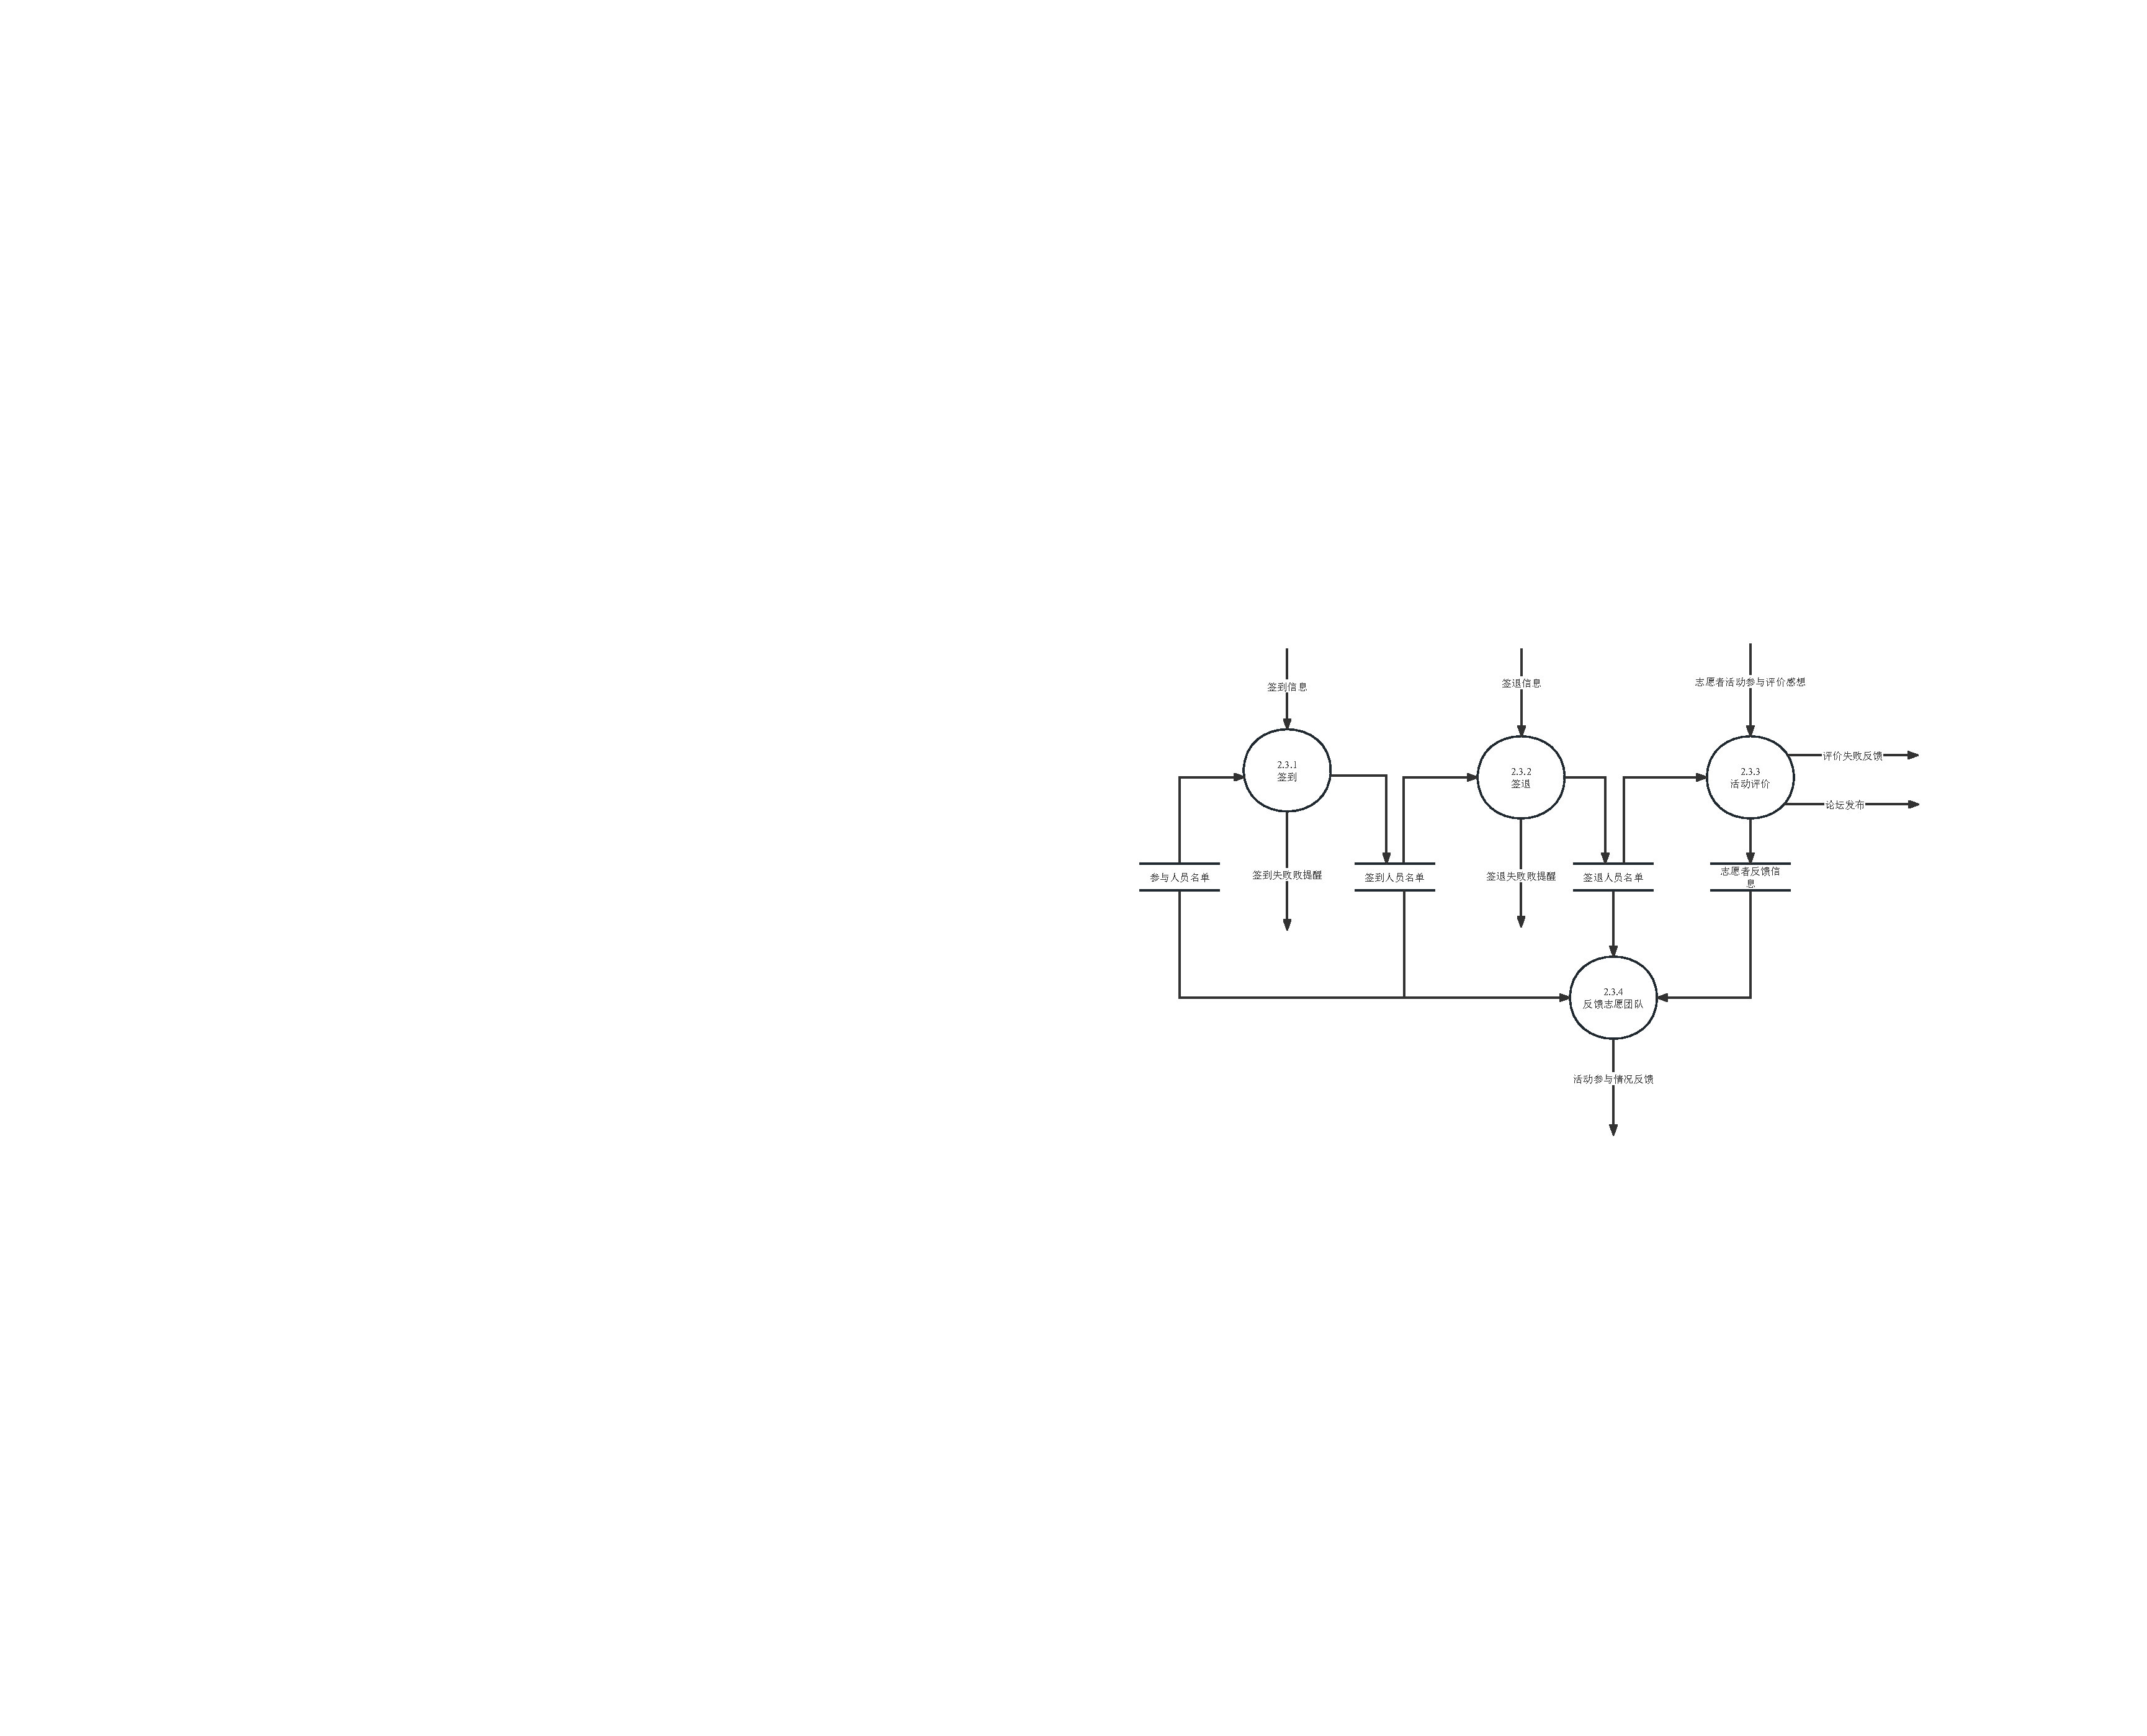
\includegraphics[width=0.95\textwidth]  {fig/志愿服务/V_2-3.2.pdf}} 
    \bicaption{志愿服务系统2层数据流图}{Data Flow Diagram for Level 2 of Volunteer Service System}
    \end{figure}

(1)数据加工词条描述说明

\begin{table}[H]  
\caption{``签到”加工词条描述}  
\begin{center}  
    \begin{tabular}{l p{11cm}} 
        \hline
        \quad 名称: & 签到\\
        \hline
        \quad 编号: & 2.3.1 \\
        \hline
        \quad 简述: & 志愿者进行签到 \\
        \hline
        \quad 输入:& 参与人员名单、签到信息 \\
        \hline
        \quad 输出:& 签到人员名单、签到失败提醒\\
        \hline
        \quad 逻辑:& 根据参与人员名单,校验用户签到信息是否正确,如错误输出签到失败信息,如正确则记录在签到人员名单。 \\
        \hline
    \end{tabular}
    \label{tab1}
\end{center}
\end{table}

\begin{algorithm}[H]
    \renewcommand{\thealgorithm}{}
    \caption{``签到”加工小说明} 
    \label{alg3} 
    \begin{algorithmic}[1]
        \IF{Pass Check 参与人员名单 then}
        \IF{Pass Check 签到信息 then}
        \STATE Generate 签到时间+签到地点 Based on 签到信息
        \STATE Write 志愿者ID+志愿项目ID+签到时间+签到地点 to 签到人员名单
        
        \ELSE return 签到失败信息
        \ENDIF
        \ELSE return 签到失败信息
        \ENDIF
    \end{algorithmic} 
\end{algorithm}


\begin{table}[H]  
\caption{``签退”加工词条描述}  
\begin{center}  
    \begin{tabular}{l p{11cm}} 
        \hline
        \quad 名称: & 签退\\
        \hline
        \quad 编号: & 2.3.2 \\
        \hline
        \quad 简述: & 志愿者进行签退 \\
        \hline
        \quad 输入:& 签到人员名单、签退信息 \\
        \hline
        \quad 输出:& 签退人员名单、签退失败提醒\\
        \hline
        \quad 逻辑:& 校验用户是否在签退人员名单中,同时校验用户签退信息是否正确,如错误输出签退失败信息,如正确则记录在签退人员名单。 \\
        \hline
    \end{tabular}
    \label{tab1}
\end{center}
\end{table}

\begin{algorithm}[H]
    \renewcommand{\thealgorithm}{}
    \caption{``签退”加工小说明} 
    \label{alg3} 
    \begin{algorithmic}[1]
        \IF{Pass Check 签退人员名单 then}
        \IF{Pass Check 签退信息 then}
        \STATE Generate 签退时间+签退地点 Based on 签退信息
        \STATE Write 志愿者ID+志愿项目ID+签退时间+签退地点 to 签退人员名单
        
        \ELSE return 签退失败信息
        \ENDIF
        \ELSE return 签退失败信息
        \ENDIF
    \end{algorithmic} 
\end{algorithm}


\begin{table}[H]  
\caption{``活动评价”加工词条描述}  
\begin{center}  
    \begin{tabular}{l p{11cm}} 
        \hline
        \quad 名称: & 活动评价\\
        \hline
        \quad 编号: & 2.3.3 \\
        \hline
        \quad 简述: & 完成签到签退的志愿者对活动进行评价 \\
        \hline
        \quad 输入:& 志愿者活动参与评价感想、签退人员名单 \\
        \hline
        \quad 输出:& 志愿者反馈信息、论坛发布\\
        \hline
        \quad 逻辑:& 校验志愿者是否完成签退,完成签退的志愿者可以提交对该志愿项目的反馈,反馈一方面会形成志愿者反馈信息,另一方面会处理后发布到论坛 \\
        \hline
    \end{tabular}
    \label{tab1}
\end{center}
\end{table}

\begin{algorithm}[H]
    \renewcommand{\thealgorithm}{}
    \caption{``活动评价”加工小说明} 
    \label{alg3} 
    \begin{algorithmic}[1]
        \IF{Pass Check 签退人员名单 then}
        \IF{Pass Check 志愿者活动参与评价感想 then}
        \STATE Generate 签退时间+签退地点 Based on 签退信息
        \STATE Write 志愿者ID+志愿项目ID+志愿者姓名+评分+文字反馈 to 志愿者反馈信息
        \ELSE return 反馈失败信息
        \ENDIF
        \ELSE return 反馈失败信息
        \ENDIF
    \end{algorithmic} 
\end{algorithm}


\begin{table}[H]  
\caption{``反馈志愿团队”加工词条描述}  
\begin{center}  
    \begin{tabular}{l p{11cm}} 
        \hline
        \quad 名称: & 反馈志愿团队\\
        \hline
        \quad 编号: & 2.3.4 \\
        \hline
        \quad 简述: & 将参与志愿者的签到、签退、活动反馈信息提供给志愿团队 \\
        \hline
        \quad 输入:& 参与人员名单、签到人员名单、签退人员名单、志愿者反馈信息 \\
        \hline
        \quad 输出:& 活动参与情况反馈\\
        \hline
        \quad 逻辑:& 统计签到率、签退率、并将用户评分以及文字反馈以匿名形式交给志愿团队 \\
        \hline
    \end{tabular}
    \label{tab1}
\end{center}
\end{table}

\begin{algorithm}[H]
    \renewcommand{\thealgorithm}{}
    \caption{``反馈志愿团队”加工小说明} 
    \label{alg3} 
    \begin{algorithmic}[1]
        \STATE Generate 签到率、签退率 Based on 参与人员名单、签到人员名单、签退人员名单
        \STATE Generate 匿名评分+匿名文字反馈 Based on 志愿者反馈信息
    \end{algorithmic} 
\end{algorithm}

(2)数据流词条描述说明

\begin{table}[H]  
    \caption{``签到信息"数据流词条描述}  
    \begin{center}  
        \begin{tabular}{l p{11cm}} 
            \hline
            \quad 名称: & 签到信息 \\
            \hline
            \quad 简述: & 志愿者进行打卡签到形成签到信息 \\
            \hline
            \quad 来源: & 源点``志愿者" \\
            \hline
            \quad 去向: & 加工``签到" \\
            \hline
            \quad 组成: & 用户ID+志愿项目ID+签到时间+签到地点  \\
            \hline
        \end{tabular}
        \label{tab1}
    \end{center}
    \end{table}


\begin{table}[H]  
    \caption{``签到失败反馈"数据流词条描述}  
    \begin{center}  
        \begin{tabular}{l p{11cm}} 
            \hline
            \quad 名称: & 签到失败反馈 \\
            \hline
            \quad 简述: & 对签到失败的志愿者发出反馈信息 \\
            \hline
            \quad 来源: & 加工``签到" \\
            \hline
            \quad 去向: & 源点``志愿者" \\
            \hline
            \quad 组成: & 用户ID+志愿项目ID+签到失败信息  \\
            \hline
        \end{tabular}
        \label{tab1}
    \end{center}
    \end{table}


\begin{table}[H]  
    \caption{``签退信息"数据流词条描述}  
    \begin{center}  
        \begin{tabular}{l p{11cm}} 
            \hline
            \quad 名称: & 签退信息 \\
            \hline
            \quad 简述: & 志愿者进行打卡签退形成签退信息 \\
            \hline
            \quad 来源: & 源点``志愿者" \\
            \hline
            \quad 去向: & 加工``签退" \\
            \hline
            \quad 组成: & 用户ID+项目ID+签退时间+签退地点  \\
            \hline
        \end{tabular}
        \label{tab1}
    \end{center}
    \end{table}


\begin{table}[H]  
    \caption{``签退失败反馈"数据流词条描述}  
    \begin{center}  
        \begin{tabular}{l p{11cm}} 
            \hline
            \quad 名称: & 签退失败反馈 \\
            \hline
            \quad 简述: & 对签退失败的志愿者发出反馈信息 \\
            \hline
            \quad 来源: & 加工``签退" \\
            \hline
            \quad 去向: & 源点``志愿者" \\
            \hline
            \quad 组成: & 用户ID+志愿项目ID+签退失败信息  \\
            \hline
        \end{tabular}
        \label{tab1}
    \end{center}
    \end{table}


\begin{table}[H]  
    \caption{``志愿者活动参与评价感想"数据流词条描述}  
    \begin{center}  
        \begin{tabular}{l p{11cm}} 
            \hline
            \quad 名称: & 志愿者活动参与评价感想 \\
            \hline
            \quad 简述: & 完成项目的志愿者对该项目进行评价反馈 \\
            \hline
            \quad 来源: & 源点``志愿者" \\
            \hline
            \quad 去向: & 加工``活动评价" \\
            \hline
            \quad 组成: & 用户ID+志愿项目ID+评价+文字反馈  \\
            \hline
        \end{tabular}
        \label{tab1}
    \end{center}
    \end{table}


\begin{table}[H]  
    \caption{``评价失败反馈"数据流词条描述}  
    \begin{center}  
        \begin{tabular}{l p{11cm}} 
            \hline
            \quad 名称: & 评价失败反馈 \\
            \hline
            \quad 简述: & 对评价失败的志愿者发出反馈信息 \\
            \hline
            \quad 来源: & 加工``签退" \\
            \hline
            \quad 去向: & 源点``志愿者" \\
            \hline
            \quad 组成: & 用户ID+志愿项目ID+评价失败信息  \\
            \hline
        \end{tabular}
        \label{tab1}
    \end{center}
    \end{table}


\begin{table}[H]  
    \caption{``论坛发布"数据流词条描述}  
    \begin{center}  
        \begin{tabular}{l p{11cm}} 
            \hline
            \quad 名称: & 论坛发布 \\
            \hline
            \quad 简述: & 志愿者提交的反馈信息在论坛发布 \\
            \hline
            \quad 来源: & 加工``活动评价" \\
            \hline
            \quad 去向: & 加工``论坛" \\
            \hline
            \quad 组成: & 志愿项目ID+评分+文字反馈  \\
            \hline
        \end{tabular}
        \label{tab1}
    \end{center}
    \end{table}



\begin{table}[H]  
    \caption{``活动参与情况反馈"数据流词条描述}  
    \begin{center}  
        \begin{tabular}{l p{11cm}} 
            \hline
            \quad 名称: & 活动参与情况反馈 \\
            \hline
            \quad 简述: & 将志愿者签到签退情况以及评价反馈提交给志愿团队 \\
            \hline
            \quad 来源: & 加工``反馈志愿团队" \\
            \hline
            \quad 去向: & 源点``志愿团队" \\
            \hline
            \quad 组成: & 志愿项目ID+签到率+签退率+评价+文字反馈  \\
            \hline
        \end{tabular}
        \label{tab1}
    \end{center}
    \end{table}


(3)文件词条描述

\begin{table}[H]
  \begin{center}
    \caption{``志愿项目签到人员名单”文件词条描述}
    %\setlength{\tabcolsep}{15mm}{
    \begin{tabular}{l p{10cm}} 
      \hline
      名称: & 志愿项目签到人员名单\\
      \hline
      简述: &  志愿者参与志愿项目的签到记录\\
      \hline
      组成: &  用户ID+志愿者姓名+项目ID+签到标记+签到时间+签到地点\\
      \hline
      存储方式: &  以用户ID为关键字\\
      \hline
    \end{tabular}
    \label{志愿项目信息表}
  \end{center}
\end{table}

\begin{table}[H]
  \begin{center}
    \caption{``志愿项目签退人员名单”文件词条描述}
    %\setlength{\tabcolsep}{15mm}{
    \begin{tabular}{l p{10cm}} 
      \hline
      名称: & 志愿项目签退人员名单\\
      \hline
      简述: &  志愿者参与志愿项目并签到之后的签退记录\\
      \hline
      组成: &  用户ID+志愿者姓名+项目ID+签退标记+签退时间+签退地点\\
      \hline
      存储方式: &  以用户ID为关键字\\
      \hline
    \end{tabular}
    \label{志愿项目信息表}
  \end{center}
\end{table}


\begin{table}[H]
  \begin{center}
    \caption{``志愿者反馈信息表”文件词条描述}
    %\setlength{\tabcolsep}{15mm}{
    \begin{tabular}{l p{10cm}} 
      \hline
      名称: & 志愿者反馈信息表\\
      \hline
      简述: &  志愿者参与志愿项目并签到和签退之后提交的反馈信息\\
      \hline
      组成: &  用户ID+志愿项目ID+志愿者姓名+评分+文字反馈\\
      \hline
      存储方式: &  以用户ID为关键字\\
      \hline
    \end{tabular}
    \label{志愿项目信息表}
  \end{center}
\end{table}

    
\subsubsection{爱心捐助系统}~{}
\\
以下是爱心捐助系统的1层数据流图、加工子图以及对应的数据字典和文件。
\begin{figure}[H]
    \center{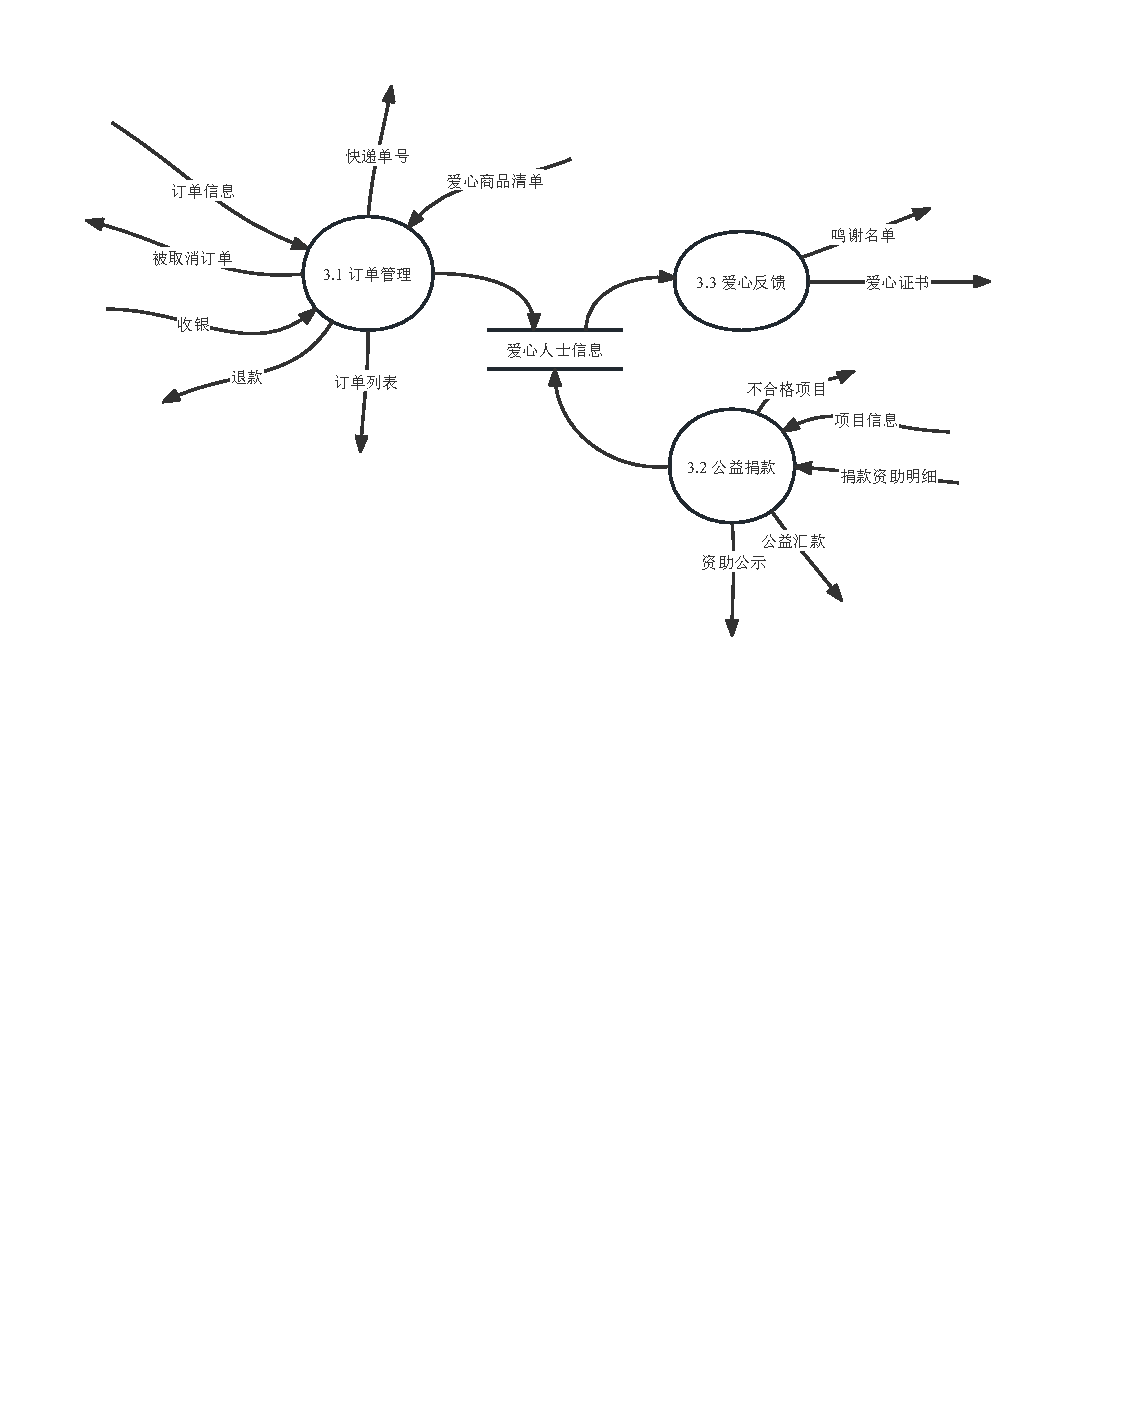
\includegraphics[width=0.95\textwidth]  {fig/爱心管理/L_1.pdf}} 
    \bicaption{爱心捐助系统1层数据流图}{Data Flow Diagram for Level 1 of Love Donation System}
    \end{figure}

\paragraph{订单管理}~{}
\begin{figure}[H]
    \center{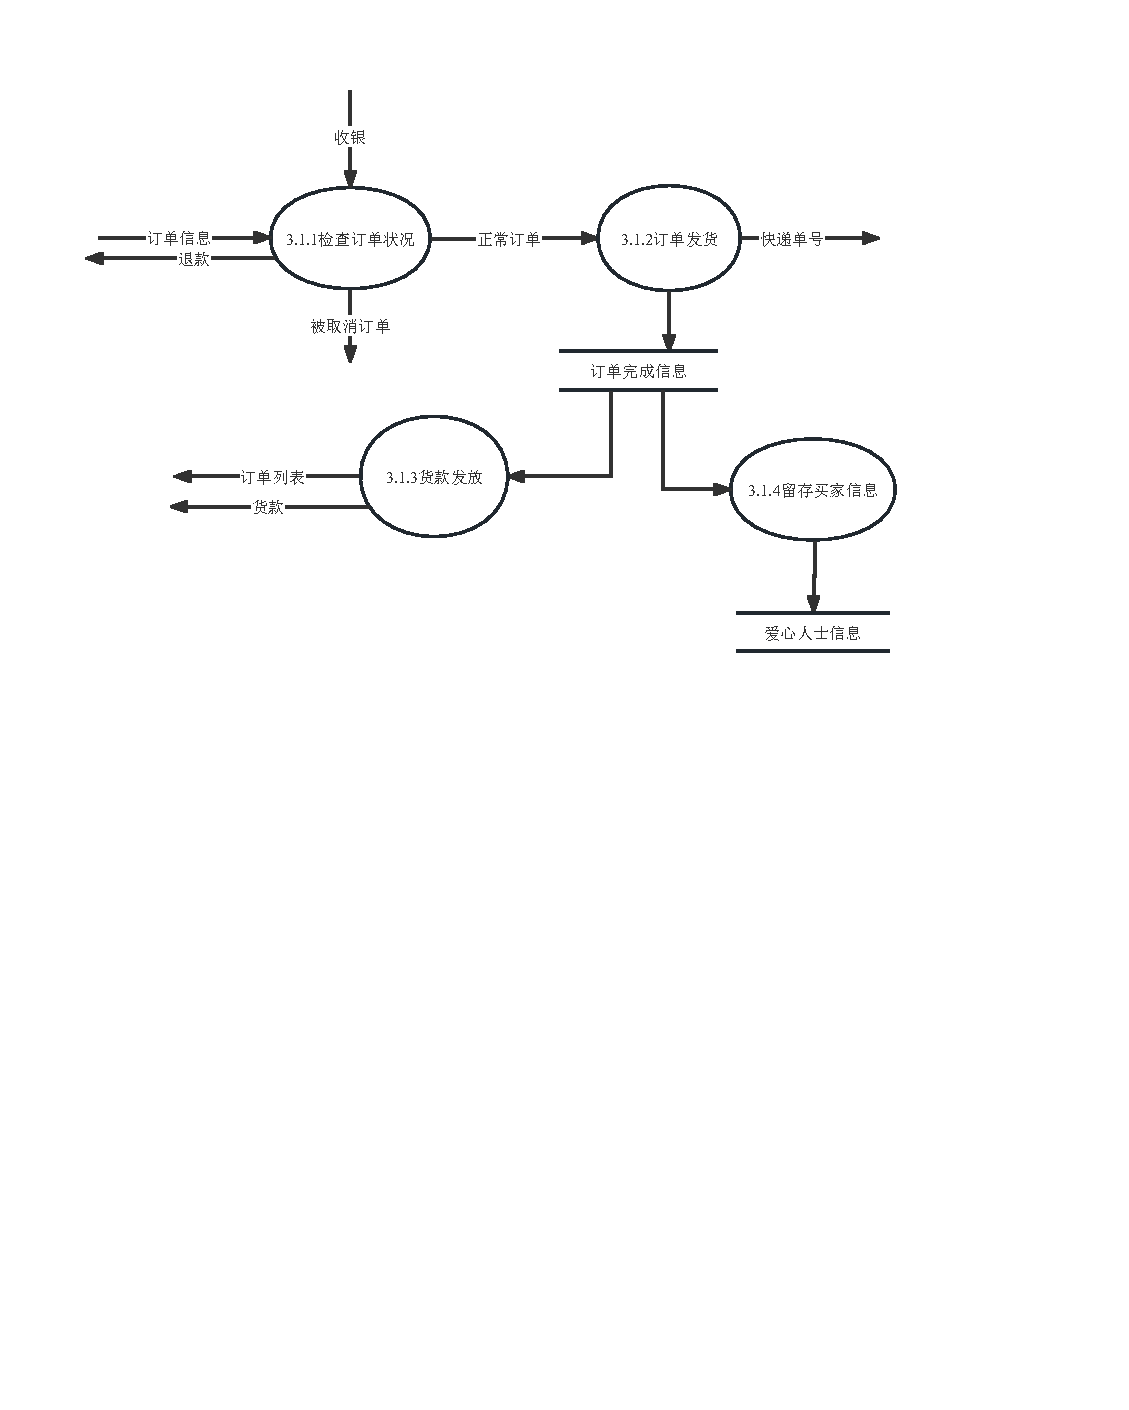
\includegraphics[width=0.95\textwidth]  {fig/爱心管理/L_2-1.pdf}} 
    \bicaption{爱心捐助系统2层数据流图}{Data Flow Diagram for Level 2 of Love Donation System}
    \end{figure}
\\

(1)数据加工词条描述说明

\begin{table}[H]  
\caption{``检查订单状况"加工词条描述}  
\begin{center}  
    \begin{tabular}{l p{11cm}} 
        \hline
        \quad 名称:  &   检查订单状况 \\
        \hline
        \quad 编号:  & 3.1.1 \\
        \hline
        \quad 简述:  & 检查用户购买商品的订单状况,是正常或是已取消 \\
        \hline
        \quad 输入:  & 订单信息、收银\\
        \hline
        \quad 输出:  & 退款、被取消订单 \\
        \hline
        \quad 逻辑:  & 根据订单信息,检查订单状况,若已取消则根据收银返回被取消订单并完成退款,正常则生成正常订单,并将收银放入资金管理账户。 \\
        \hline
    \end{tabular}
    \label{tab1}
\end{center}
\end{table}

\begin{algorithm}[H]
    \renewcommand{\thealgorithm}{}
    \caption{“检查订单状况”加工小说明} 
    \label{alg3} 
    \begin{algorithmic}[1]
        \IF{Pass Check 订单信息} 
        \STATE Generate 正常订单信息 Based on 订单信息
        \STATE Put 收银 into 资金管理账户
        \ELSE
        \STATE Generate 正常订单信息 Based on 被取消订单信息
        \STATE Do 退款 and Return 收银
        \ENDIF 
    \end{algorithmic} 
\end{algorithm}

\begin{table}[H]  
\caption{``订单发货"加工词条描述}  
\begin{center}  
    \begin{tabular}{l p{11cm}} 
        \hline
        \quad 名称:  &   订单发货 \\
        \hline
        \quad 编号:  & 3.1.2 \\
        \hline
        \quad 简述:  & 将用户所下的正常订单进行发货 \\
        \hline
        \quad 输入:  & 正常订单 \\
        \hline
        \quad 输出:  & 快递单号、订单完成信息 \\
        \hline
        \quad 逻辑:  & 通过正常订单中填写的收件人、电话和配送地址等信息,会自动生成配送单,匹配快递公司并交由其进行处理,生成快递单号,安排出货和配送。同时,返回快递公司给出的快递单号,最后将发货完成的汇总到订单完成信息中。 \\
        \hline
    \end{tabular}
    \label{tab1}
\end{center}
\end{table}

\begin{algorithm}[H]
    \renewcommand{\thealgorithm}{}
    \caption{“订单发货”加工小说明} 
    \label{alg3} 
    \begin{algorithmic}[1] 
        \STATE Get 收件人、电话和配送地址等信息 of 正常订单
        \STATE Generate 配送单
        \STATE Match 快递公司
        \STATE Generate 快递单号 and Arrange 出货配送
        \STATE Summarize 发货信息 to 订单完成信息 
    \end{algorithmic} 
\end{algorithm}

\begin{table}[H]  
\caption{``货款发放"加工词条描述}  
\begin{center}  
    \begin{tabular}{l p{11cm}} 
        \hline
        \quad 名称:  &   货款发放 \\
        \hline
        \quad 编号:  & 3.1.3 \\
        \hline
        \quad 简述:  & 将用户购买商品的货款付给对应爱心商户 \\
        \hline
        \quad 输入:  & 订单完成信息 \\
        \hline
        \quad 输出:  & 货款、订单列表 \\
        \hline
        \quad 逻辑:  & 根据订单完成信息,系统将对应的款项和对应的商户进行匹配,将货款打入商户的账户,并生成完结订单列表。 \\
        \hline
    \end{tabular}
    \label{tab1}
\end{center}
\end{table}


\begin{algorithm}[H]
    \renewcommand{\thealgorithm}{}
    \caption{“货款发放”加工小说明} 
    \label{alg3} 
    \begin{algorithmic}[1] 
        \STATE Get 款项和商户信息 of 订单完成信息
        \STATE Match 对应商户ID
        \STATE Add 货款 to 对应商户账户
        \STATE Generate 完结订单列表
    \end{algorithmic} 
\end{algorithm}

\begin{table}[H]  
\caption{``留存买家信息"加工词条描述}  
\begin{center}  
    \begin{tabular}{l p{11cm}} 
        \hline
        \quad 名称:  &   留存买家信息 \\
        \hline
        \quad 编号:  & 3.1.4 \\
        \hline
        \quad 简述:  & 将用户所下的正常订单进行发货 \\
        \hline
        \quad 输入:  & 订单完成信息 \\
        \hline
        \quad 输出:  & 快递单号、订单完成信息 \\
        \hline
        \quad 逻辑:  & 订单完成后,留存订单完成信息中的付款金额和用户名,作为爱心人士信息,用作爱心反馈操作。 \\
        \hline
    \end{tabular}
    \label{tab1}
\end{center}
\end{table}

\begin{algorithm}[H]
    \renewcommand{\thealgorithm}{}
    \caption{“留存买家信息”加工小说明} 
    \label{alg3} 
    \begin{algorithmic}[1] 
        \STATE Get 付款金额和用户名 of 订单完成信息
        \STATE Save 付款金额和用户名 as 爱心人士信息
    \end{algorithmic} 
\end{algorithm}

(2)数据流词条描述说明
\begin{table}[H]  
    \caption{``订单信息"数据流词条描述}  
    \begin{center}  
        \begin{tabular}{l p{11cm}} 
            \hline
            \quad 名称:  &   订单信息 \\
            \hline
            \quad 简述:  & 用户购买商品,系统生成订单的信息 \\
            \hline
            \quad 来源:  & 源点``公益商户" \\
            \hline
            \quad 去向:  & 加工``检查订单状况" \\
            \hline
            \quad 组成:  & 订单ID+商品ID+公益商家ID+用户ID+用户名+收件人+联系方式+发货地址+下单时间 \\
            \hline
        \end{tabular}
        \label{tab1}
    \end{center}
    \end{table}
    
    
    \begin{table}[H]  
    \caption{``收银"数据流词条描述}  
    \begin{center}  
        \begin{tabular}{l p{11cm}} 
            \hline
            \quad 名称:  &   收银 \\
            \hline
            \quad 简述:  & 用户购买商品的付款 \\
            \hline
            \quad 来源:  & 源点``购物者" \\
            \hline
            \quad 去向:  & 加工``检查订单状况" \\
            \hline
            \quad 组成:  & 付款金额+支付方式  \\
            \hline
        \end{tabular}
        \label{tab1}
    \end{center}
    \end{table}
    
    \begin{table}[H]  
    \caption{``被取消订单"数据流词条描述}  
    \begin{center}  
        \begin{tabular}{l p{11cm}} 
            \hline
            \quad 名称:  &   被取消订单 \\
            \hline
            \quad 简述:  & 检查订单状况后发现状态为已取消的订单 \\
            \hline
            \quad 来源:  & 加工``检查订单状况" \\
            \hline
            \quad 去向:  & 源点``公益商户" \\
            \hline
            \quad 组成:  & 订单信息  \\
            \hline
        \end{tabular}
        \label{tab1}
    \end{center}
    \end{table}
    
    \begin{table}[H]  
    \caption{``退款"数据流词条描述}  
    \begin{center}  
        \begin{tabular}{l p{11cm}} 
            \hline
            \quad 名称:  &   退款 \\
            \hline
            \quad 简述:  & 订单取消后对用户付款的退还 \\
            \hline
            \quad 来源:  & 加工``检查订单状况" \\
            \hline
            \quad 去向:  & 源点``购物者" \\
            \hline
            \quad 组成:  & 收银  \\
            \hline
        \end{tabular}
        \label{tab1}
    \end{center}
    \end{table}
    
    \begin{table}[H]  
    \caption{``正常订单"数据流词条描述}  
    \begin{center}  
        \begin{tabular}{l p{11cm}} 
            \hline
            \quad 名称:  &   正常订单 \\
            \hline
            \quad 简述:  & 检查订单状况后未被取消的订单 \\
            \hline
            \quad 来源:  & 加工``检查订单状况" \\
            \hline
            \quad 去向:  & 加工``订单发货" \\
            \hline
            \quad 组成:  & 订单信息  \\
            \hline
        \end{tabular}
        \label{tab1}
    \end{center}
    \end{table}
    
    \begin{table}[H]  
    \caption{``快递单号"数据流词条描述}  
    \begin{center}  
        \begin{tabular}{l p{11cm}} 
            \hline
            \quad 名称:  &   快递单号 \\
            \hline
            \quad 简述:  & 正常订单完成发货后的物流单号 \\
            \hline
            \quad 来源:  & 加工``订单发货" \\
            \hline
            \quad 去向:  &  源点``购物者"\\
            \hline
            \quad 组成:  & 快递公司ID+物流单号  \\
            \hline
        \end{tabular}
        \label{tab1}
    \end{center}
    \end{table}
    
    \begin{table}[H]  
    \caption{``订单列表"数据流词条描述}  
    \begin{center}  
        \begin{tabular}{l p{11cm}} 
            \hline
            \quad 名称:  &   订单列表 \\
            \hline
            \quad 简述:  & 货款发放后的完结的订单汇总 \\
            \hline
            \quad 来源:  & 文件``订单完成信息" \\
            \hline
            \quad 去向:  & 源点``爱心商户" \\
            \hline
            \quad 组成:  & 订单ID+商品ID+公益商家ID+用户ID+完结时间 \\
            \hline
        \end{tabular}
        \label{tab1}
    \end{center}
    \end{table}
    
    

(3)文件词条描述
\begin{table}[H]  
\caption{``订单完成情况”文件描述}  
\begin{center}  
    \begin{tabular}{l p{11cm}} 
        \hline
        \quad 名称:  &   订单完成情况 \\
        \hline
        \quad 简述:  & 存储购物者商品发货后的订单完成信息\\
        \hline
        \quad 组成:  & 订单ID+付款金额+商品ID+公益商家ID+用户ID+用户名+下单时间 \\
        \hline
        \quad 存储方式:  & 以订单ID为关键字。 \\
        \hline
    \end{tabular}
    \label{tab1}
\end{center}
\end{table}

\begin{table}[H]  
\caption{``爱心人士信息”文件描述}  
\begin{center}  
    \begin{tabular}{l p{11cm}} 
        \hline
        \quad 名称:  &   爱心人士信息 \\
        \hline
        \quad 简述:  & 存储购买爱心商品的爱心人士信息\\
        \hline
        \quad 组成:  & 用户ID+用户名+付款金额 \\
        \hline
        \quad 存储方式:  & 以用户ID为关键字。 \\
        \hline
    \end{tabular}
    \label{tab1}
\end{center}
\end{table}


\paragraph{捐款管理}~{}
\begin{figure}[H]
    \center{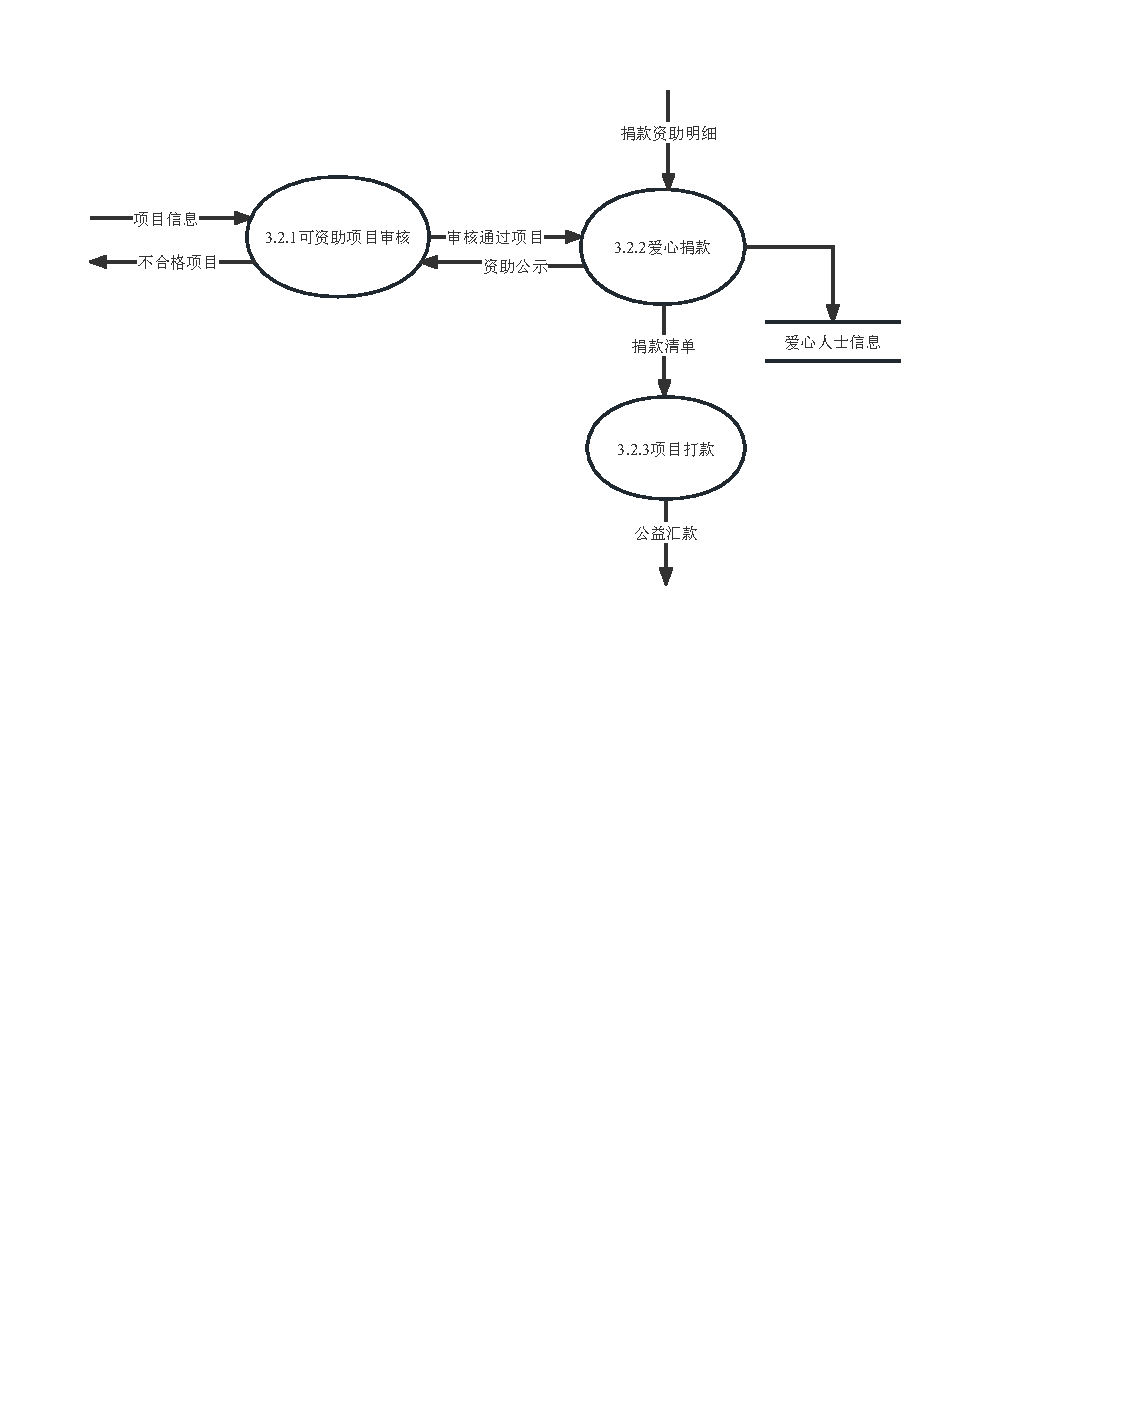
\includegraphics[width=0.95\textwidth]  {fig/爱心管理/L_2-2.pdf}} 
    \bicaption{爱心捐助系统2层数据流图}{Data Flow Diagram for Level 2 of Love Donation System}
    \end{figure}
\\

(1)数据加工词条描述说明
\begin{table}[H]  
    \caption{``可资助项目审核"加工词条描述}  
    \begin{center}  
        \begin{tabular}{l p{11cm}} 
            \hline
            \quad 名称:  &   可资助项目审核 \\
            \hline
            \quad 编号:  & 3.2.1 \\
            \hline
            \quad 简述:  & 审核志愿项目,确定合规、可资助的项目 \\
            \hline
            \quad 输入:  & 项目信息\\
            \hline
            \quad 输出:  & 审核通过项目、不合格项目 \\
            \hline
            \quad 逻辑:  & 根据项目信息,检查项目资质,若检查不合格则返回不合格项目,合格则生成审核通过项目。 \\
            \hline
        \end{tabular}
        \label{tab1}
    \end{center}
    \end{table}

\begin{algorithm}[H]
    \renewcommand{\thealgorithm}{}
    \caption{“可资助项目审核”加工小说明} 
    \label{alg3} 
    \begin{algorithmic}[1]
        \IF{Pass Check 项目信息} 
        \STATE Generate 审核通过项目信息 Based on 项目信息
        \ELSE
        \STATE Generate 不合格项目信息 Based on 项目信息
        \STATE Return 不合格项目信息
        \ENDIF 
    \end{algorithmic} 
\end{algorithm}
    
    \begin{table}[H]  
    \caption{``爱心捐款"加工词条描述}  
    \begin{center}  
        \begin{tabular}{l p{11cm}} 
            \hline
            \quad 名称:  &   爱心捐款 \\
            \hline
            \quad 编号:  & 3.2.2 \\
            \hline
            \quad 简述:  & 管理爱心人士对志愿项目的捐款 \\
            \hline
            \quad 输入:  & 捐款资助明细、审核通过项目\\
            \hline
            \quad 输出:  & 资助公示、捐助清单、爱心人士信息 \\
            \hline
            \quad 逻辑:  & 用于接收和管理爱心人士对某志愿项目的捐款,将某项目的资助进行汇总,并对款项进行公示,再留存捐款资助明细中的捐款金额和用户名,作为爱心人士信息,用作爱心反馈操作。 \\
            \hline
        \end{tabular}
        \label{tab1}
    \end{center}
    \end{table}

\begin{algorithm}[H]
    \renewcommand{\thealgorithm}{}
    \caption{“爱心捐款”加工小说明} 
    \label{alg3} 
    \begin{algorithmic}[1] 
        \STATE Select Sum(资助捐款)as 项目资助 Group by 志愿项目
        \STATE Generate 资助公示 Base on 项目资助
        \STATE Save 捐款金额和用户名 as 爱心人士信息 Base on 捐款资助明细
    \end{algorithmic} 
\end{algorithm}
    
    \begin{table}[H]  
    \caption{``项目打款"加工词条描述}  
    \begin{center}  
        \begin{tabular}{l p{11cm}} 
            \hline
            \quad 名称:  &   项目打款 \\
            \hline
            \quad 编号:  & 3.2.3 \\
            \hline
            \quad 简述:  & 将爱心人士的捐款转给对应志愿团队 \\
            \hline
            \quad 输入:  & 捐款清单 \\
            \hline
            \quad 输出:  & 公益汇款 \\
            \hline
            \quad 逻辑:  & 资金汇总后后,通过捐款清单中的项目编号,志愿团队名和捐款金额汇总,统一打款给对应志愿团队。 \\
            \hline
        \end{tabular}
        \label{tab1}
    \end{center}
    \end{table}
    
\begin{algorithm}[H]
    \renewcommand{\thealgorithm}{}
    \caption{“项目打款”加工小说明} 
    \label{alg3} 
    \begin{algorithmic}[1] 
        \STATE Match 项目ID、志愿团队名和捐款金额汇总 of 捐款清单
        \STATE Add 捐款 to 对应团队账户
    \end{algorithmic} 
\end{algorithm}

(2)数据流词条描述说明
\begin{table}[H]  
    \caption{``鸣谢名单"数据流词条描述}  
    \begin{center}  
        \begin{tabular}{l p{11cm}} 
            \hline
            \quad 名称:  &  鸣谢名单 \\
            \hline
            \quad 简述:  & 汇总爱心人士的名单,以便爱心商户和志愿团队感谢\\
            \hline
            \quad 来源:  & 文件``爱心买家名单" \\
            \hline
            \quad 去向:  & 源点``爱心商户"、源点``志愿团队" \\
            \hline
            \quad 组成:  & 用户名+感谢语 \\
            \hline
        \end{tabular}
        \label{tab1}
    \end{center}
    \end{table}
    
    
    \begin{table}[H]  
    \caption{``爱心证书"数据流词条描述}  
    \begin{center}  
        \begin{tabular}{l p{11cm}} 
            \hline
            \quad 名称:  &   爱心证书 \\
            \hline
            \quad 简述:  & 爱心人士风险爱心的证明 \\
            \hline
            \quad 来源:  & 文件``爱心买家名单" \\
            \hline
            \quad 去向:  & 加工``检查订单状况" \\
            \hline
            \quad 组成:  & 用户ID+用户名+证书生成时间+证明文字  \\
            \hline
        \end{tabular}
        \label{tab1}
    \end{center}
    \end{table}
    
    
    

(3)文件词条描述

\begin{table}[H]  
\caption{``爱心人士信息”文件描述}  
\begin{center}  
    \begin{tabular}{l p{11cm}} 
        \hline
        \quad 名称:  &   爱心人士信息 \\
        \hline
        \quad 简述:  & 存储为志愿项目捐款的爱心人士信息\\
        \hline
        \quad 组成:  & 用户ID+用户名+捐款金额 \\
        \hline
        \quad 存储方式:  & 以用户ID为关键字。 \\
        \hline
    \end{tabular}
    \label{tab1}
\end{center}
\end{table}


\paragraph{爱心反馈管理}~{}
\begin{figure}[H]
    \center{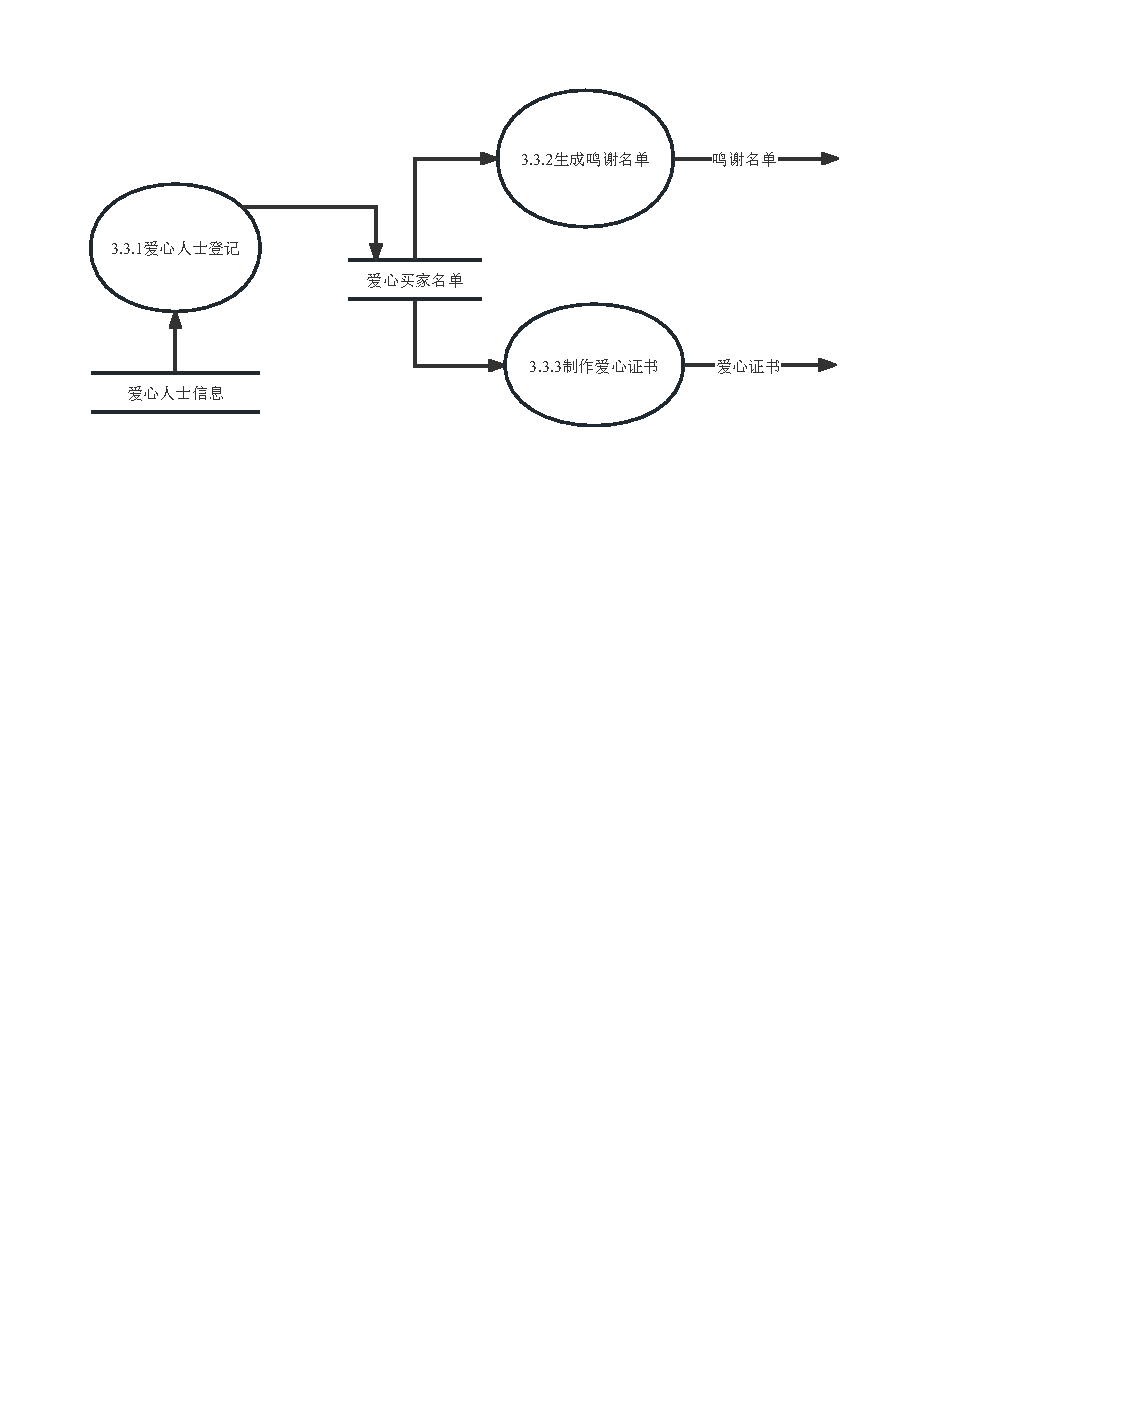
\includegraphics[width=0.95\textwidth]  {fig/爱心管理/L_2-3.pdf}} 
    \bicaption{爱心捐助系统2层数据流图}{Data Flow Diagram for Level 2 of Love Donation System}
    \end{figure}
\\

(1)数据加工词条描述说明
\begin{table}[H]  
    \caption{``爱心人士登记"加工词条描述}  
    \begin{center}  
        \begin{tabular}{l p{11cm}} 
            \hline
            \quad 名称:  &   爱心人士登记 \\
            \hline
            \quad 编号:  & 3.3.1 \\
            \hline
            \quad 简述:  & 登记爱心人士,以便爱心反馈 \\
            \hline
            \quad 输入:  & 爱心人士信息\\
            \hline
            \quad 输出:  & 爱心买家名单 \\
            \hline
            \quad 逻辑:  & 根据爱心人士信息,录入爱心买家并生成名单。 \\
            \hline
        \end{tabular}
        \label{tab1}
    \end{center}
    \end{table}

\begin{algorithm}[H]
    \renewcommand{\thealgorithm}{}
    \caption{“爱心人士登记”加工小说明} 
    \label{alg3} 
    \begin{algorithmic}[1] 
        \STATE Generate 爱心买家名单 Base on 爱心人士信息
    \end{algorithmic} 
\end{algorithm}
    
    \begin{table}[H]  
    \caption{``生成鸣谢名单"加工词条描述}  
    \begin{center}  
        \begin{tabular}{l p{11cm}} 
            \hline
            \quad 名称:  &   生成鸣谢名单 \\
            \hline
            \quad 编号:  & 3.3.2 \\
            \hline
            \quad 简述:  & 生成购买爱心商品和项目捐款的爱心人士名单,加以鸣谢 \\
            \hline
            \quad 输入:  & 爱心买家名单 \\
            \hline
            \quad 输出:  & 鸣谢名单 \\
            \hline
            \quad 逻辑:  & 为名单中所有用户名匹配一句特有的感谢语,生成鸣谢名单。 \\
            \hline
        \end{tabular}
        \label{tab1}
    \end{center}
    \end{table}

\begin{algorithm}[H]
    \renewcommand{\thealgorithm}{}
    \caption{“生成鸣谢名单”加工小说明} 
    \label{alg3} 
    \begin{algorithmic}[1] 
        \STATE Get 用户名 of 爱心买家名单
        \STATE Generate 感谢语
        \STATE Save 用户名和感谢语 as 鸣谢名单
    \end{algorithmic} 
\end{algorithm}
    
    \begin{table}[H]  
    \caption{``制作爱心证书"加工词条描述}  
    \begin{center}  
        \begin{tabular}{l p{11cm}} 
            \hline
            \quad 名称:  &   制作爱心证书 \\
            \hline
            \quad 编号:  & 3.3.3 \\
            \hline
            \quad 简述:  & 制作感谢爱心人士的爱心证书 \\
            \hline
            \quad 输入:  & 爱心买家名单 \\
            \hline
            \quad 输出:  & 爱心证书 \\
            \hline
            \quad 逻辑:  & 将用户名和感谢语输入定制的证书模板中,形成爱心证书。 \\
            \hline
        \end{tabular}
        \label{tab1}
    \end{center}
    \end{table}

\begin{algorithm}[H]
    \renewcommand{\thealgorithm}{}
    \caption{“制作爱心证书”加工小说明} 
    \label{alg3} 
    \begin{algorithmic}[1] 
        \STATE Select 证书模板
        \STATE Generate 爱心证书 from 用户名、感谢语和证书模板
    \end{algorithmic} 
\end{algorithm}

(2)数据流词条描述说明
\begin{table}[H]  
\caption{``项目信息"数据流词条描述}  
\begin{center}  
    \begin{tabular}{l p{11cm}} 
        \hline
        \quad 名称:  &   项目信息 \\
        \hline
        \quad 简述:  & 志愿团队提交资助志愿项目的信息 \\
        \hline
        \quad 来源:  & 源点``志愿团队" \\
        \hline
        \quad 去向:  & 加工``可资助项目审核" \\
        \hline
        \quad 组成:  & 项目ID+志愿团队ID+项目时间+可报名人数+项目描述 \\
        \hline
    \end{tabular}
    \label{tab1}
\end{center}
\end{table}


\begin{table}[H]  
\caption{``不合格项目"数据流词条描述}  
\begin{center}  
    \begin{tabular}{l p{11cm}} 
        \hline
        \quad 名称:  &  不合格项目 \\
        \hline
        \quad 简述:  & 经系统审核后,不合格的受资助项目 \\
        \hline
        \quad 来源:  & 加工``可资助项目审核"\\
        \hline
        \quad 去向:  & 加工``爱心捐助" \\
        \hline
        \quad 组成:  & 项目信息  \\
        \hline
    \end{tabular}
    \label{tab1}
\end{center}
\end{table}

\begin{table}[H]  
\caption{``审核通过项目"数据流词条描述}  
\begin{center}  
    \begin{tabular}{l p{11cm}} 
        \hline
        \quad 名称:  &   审核通过项目 \\
        \hline
        \quad 简述:  & 经系统审核后,合格的受资助项目 \\
        \hline
        \quad 来源:  & 加工``爱心捐款" \\
        \hline
        \quad 去向:  & 加工``可资助项目审核" \\
        \hline
        \quad 组成:  & 项目信息  \\
        \hline
    \end{tabular}
    \label{tab1}
\end{center}
\end{table}

\begin{table}[H]  
\caption{``捐款资助明细"数据流词条描述}  
\begin{center}  
    \begin{tabular}{l p{11cm}} 
        \hline
        \quad 名称:  &   捐款资助明细 \\
        \hline
        \quad 简述:  & 捐款者对志愿项目的捐款信息 \\
        \hline
        \quad 来源:  & 源点``捐款人" \\
        \hline
        \quad 去向:  & 加工``爱心捐款" \\
        \hline
        \quad 组成:  & 项目ID+用户ID+用户名+捐款金额+支付方式+捐款留言  \\
        \hline
    \end{tabular}
    \label{tab1}
\end{center}
\end{table}

\begin{table}[H]  
\caption{``资助公示"数据流词条描述}  
\begin{center}  
    \begin{tabular}{l p{11cm}} 
        \hline
        \quad 名称:  &   资助公示 \\
        \hline
        \quad 简述:  & 对资助项目的受资助情况进行公示 \\
        \hline
        \quad 来源:  & 加工``爱心捐款" \\
        \hline
        \quad 去向:  & 源点``政府相关部门" \\
        \hline
        \quad 组成:  & 志愿团队ID+项目描述+资助金额  \\
        \hline
    \end{tabular}
    \label{tab1}
\end{center}
\end{table}

\begin{table}[H]  
\caption{``捐款清单"数据流词条描述}  
\begin{center}  
    \begin{tabular}{l p{11cm}} 
        \hline
        \quad 名称:  &  捐款清单 \\
        \hline
        \quad 简述:  & 项目获得的爱心捐款汇总 \\
        \hline
        \quad 来源:  & 加工``爱心捐款" \\
        \hline
        \quad 去向:  &  加工``项目打款"\\
        \hline
        \quad 组成:  & 志愿团队ID+项目ID+资助金额  \\
        \hline
    \end{tabular}
    \label{tab1}
\end{center}
\end{table}

\begin{table}[H]  
\caption{``公益汇款"数据流词条描述}  
\begin{center}  
    \begin{tabular}{l p{11cm}} 
        \hline
        \quad 名称:  &  公益汇款 \\
        \hline
        \quad 简述:  & 对公益项目对应的志愿团队进行捐款发放 \\
        \hline
        \quad 来源:  & 加工``项目打款" \\
        \hline
        \quad 去向:  & 源点``志愿团队" \\
        \hline
        \quad 组成:  & 志愿团队ID+资助金额 \\
        \hline
    \end{tabular}
    \label{tab1}
\end{center}
\end{table}



(3)文件词条描述

\begin{table}[H]  
\caption{``爱心人士信息”文件描述}  
\begin{center}  
    \begin{tabular}{l p{11cm}} 
        \hline
        \quad 名称:  &   爱心人士信息 \\
        \hline
        \quad 简述:  & 存储购买爱心商品的爱心人士信息\\
        \hline
        \quad 组成:  & 用户ID+用户名+[付款金额|捐款金额] \\
        \hline
        \quad 存储方式:  & 以用户ID为关键字。 \\
        \hline
    \end{tabular}
    \label{tab1}
\end{center}
\end{table}

\begin{table}[H]  
\caption{``爱心买家名单”文件描述}  
\begin{center}  
    \begin{tabular}{l p{11cm}} 
        \hline
        \quad 名称:  &   订单完成情况 \\
        \hline
        \quad 简述:  & 存储为爱心付费买家的名单用于感谢\\
        \hline
        \quad 组成:  & 用户名+[付款金额|捐款金额] \\
        \hline
        \quad 存储方式:  & 以用户名为关键字。 \\
        \hline
    \end{tabular}
    \label{tab1}
\end{center}
\end{table}

\subsubsection{公益课程系统}
以下是公益课程系统的1层数据流图、加工子图以及对应的数据字典和文件。
\begin{figure}[H]
    \center{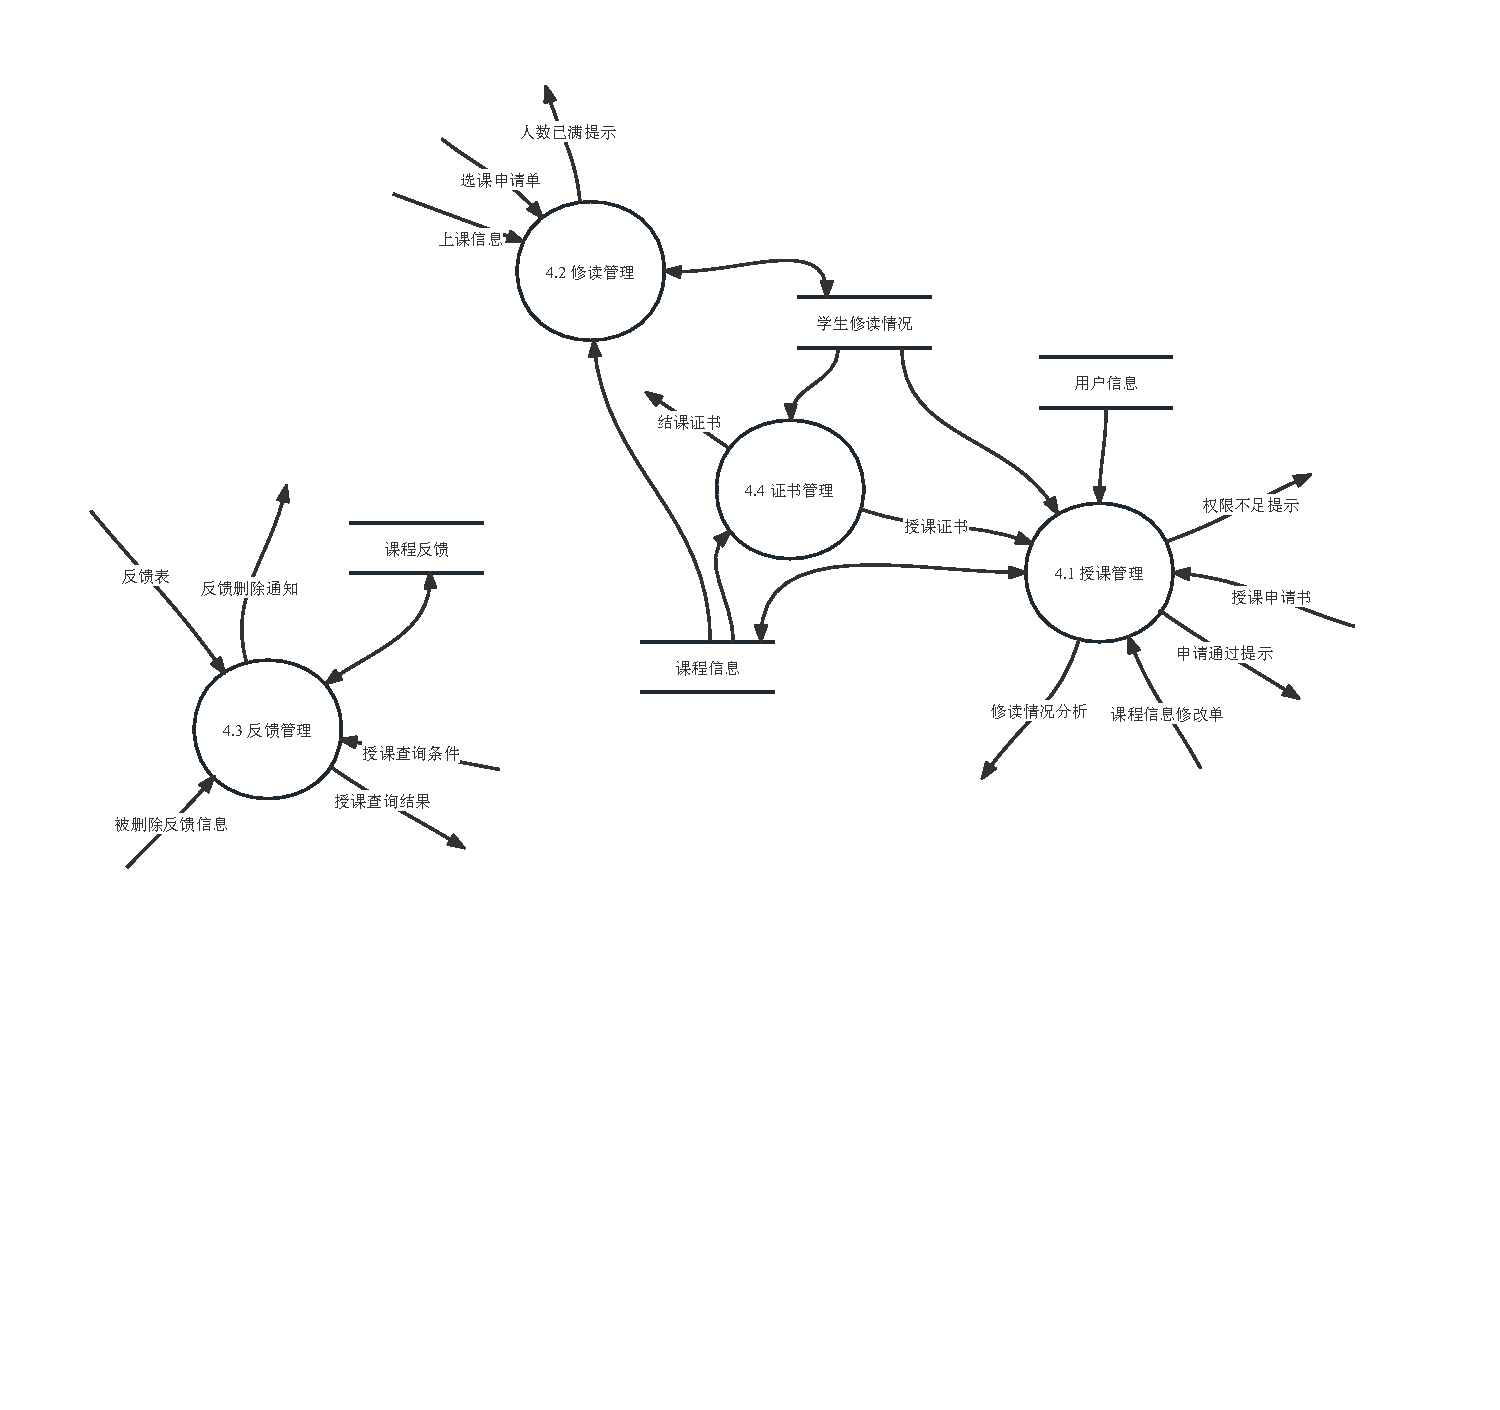
\includegraphics[width=0.95\textwidth]  {fig/课程管理/C_1.pdf}} 
    \bicaption{公益课程系统1层数据流图}{Data Flow Diagram for Level 1 of Public Course System}
    \end{figure}
    
\paragraph{授课管理}~{}
\\

\begin{figure}[H]
    \center{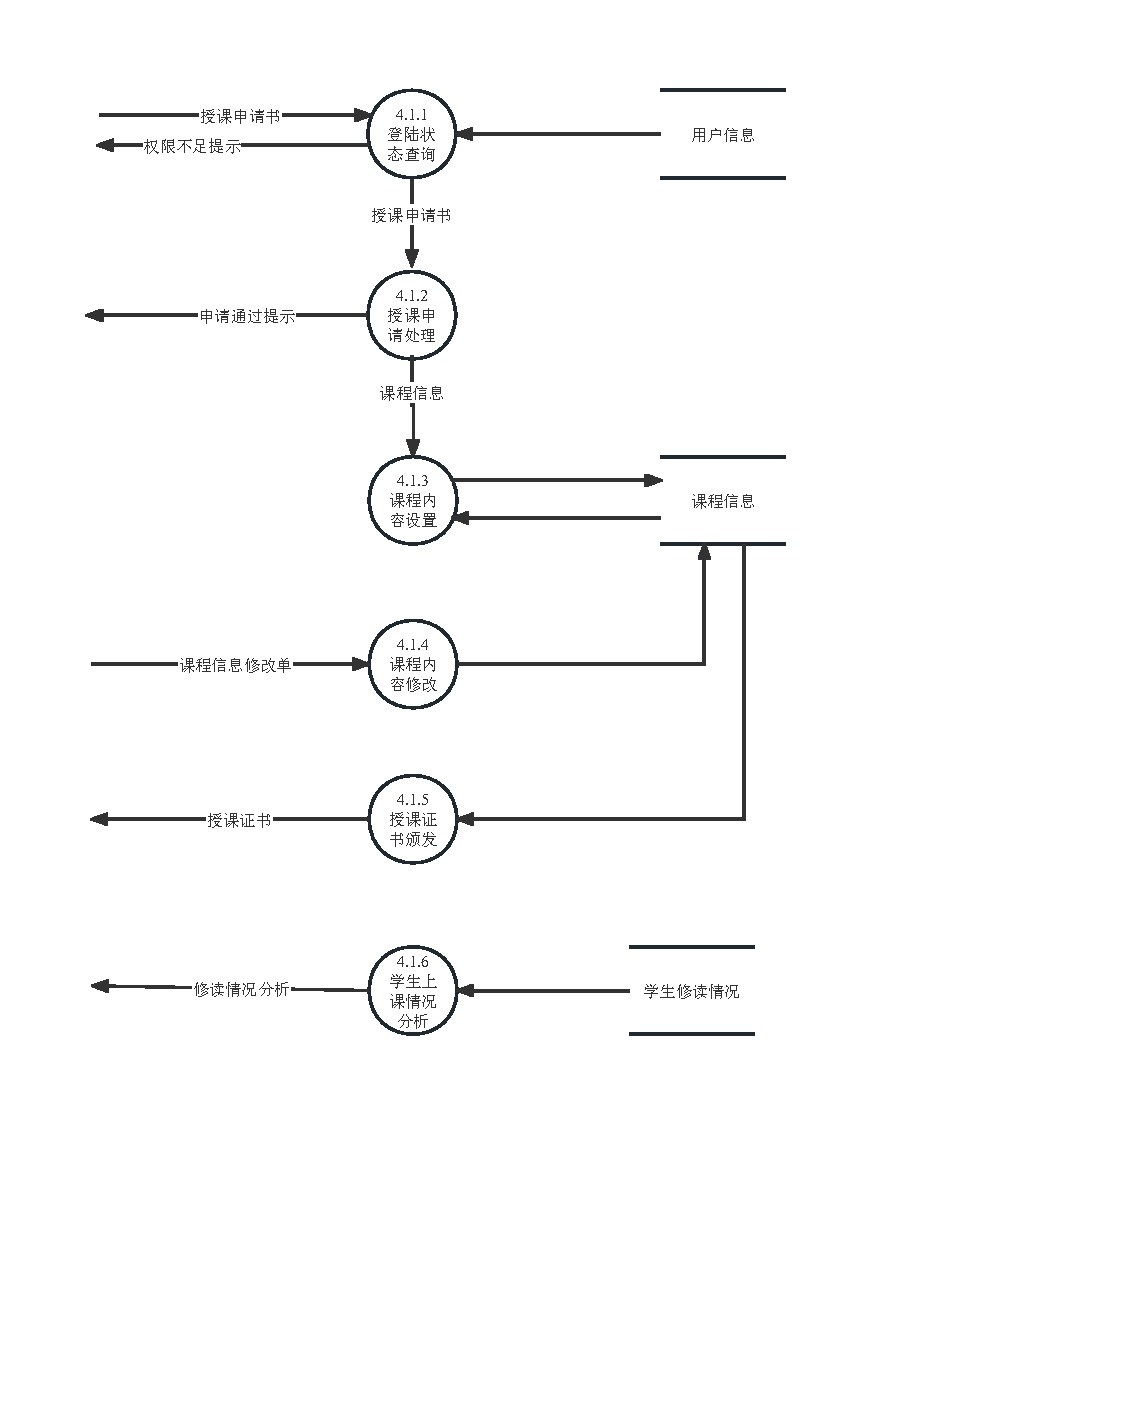
\includegraphics[width=0.95\textwidth]  {fig/课程管理/C_2-1.pdf}} 
    \bicaption{公益课程系统2层数据流图}{Data Flow Diagram for Level 2 of Public Course System}
    \end{figure}

(1)数据加工词条描述说明
\begin{table}[H]  
\caption{“登录权限查询”加工词条描述}  
\begin{center}  
    \begin{tabular}{l p{11cm}} 
        \hline
        \quad 名称: & 登录权限查询 \\
        \hline
        \quad 编号: & 4.1.1 \\
        \hline
        \quad 简述: & 查询用户登录权限的功能 \\
        \hline
        \quad 输入: & 授课申请书、已登录用户权限、用户ID \\
        \hline
        \quad 输出: & 登录状态、权限不足提示、用户名 \\
        \hline
        \quad 逻辑: & 查询对应用户ID的权限信息。 \\
        \hline
    \end{tabular}
    \label{tab1}
\end{center}
\end{table}


\begin{algorithm}[H] 
    \renewcommand{\thealgorithm}{}
    \caption{“登录权限查询”加工小说明} 
    \label{alg3} 
    \begin{algorithmic}[1]
        \STATE Get 系统时间 As 查询时间
        \STATE Write 账号 + 密码 + 登录状态  To 登录权限查询信息 
    \end{algorithmic} 
\end{algorithm}

\begin{table}[H]  
\caption{“授课申请处理”加工词条描述}  
\begin{center}  
    \begin{tabular}{l p{11cm}} 
        \hline
        \quad 名称: & 授课申请处理 \\
        \hline
        \quad 编号: & 4.1.2 \\
        \hline
        \quad 简述: & 处理授课申请的功能 \\
        \hline
        \quad 输入: & 授课申请书、用户ID \\
        \hline
        \quad 输出: & 申请通过提示、申请处理时间、课程名、课程信息 \\
        \hline
        \quad 逻辑: & 通过对授课申请书处理申请、建立课程信息 \\
        \hline
    \end{tabular}
    \label{tab1}
\end{center}
\end{table}


\begin{algorithm}[H]
    \renewcommand{\thealgorithm}{}
    \caption{“授课申请处理”加工小说明} 
    \label{alg3} 
    \begin{algorithmic}[1]
        \IF{授课申请处理通过} 
        \STATE Write 用户ID to 授课人信息 
        \STATE Write {理由} + 反应时间  To 申请通过提示
        \ELSE
        \STATE Write {理由} + 反应时间  To 授课申请处理反馈
        \ENDIF 
    \end{algorithmic} 
\end{algorithm}


\begin{table}[H]  
\caption{“课程内容设置”加工词条描述}  
\begin{center}  
    \begin{tabular}{l p{11cm}} 
        \hline
        \quad 名称: & 课程内容设置 \\
        \hline
        \quad 编号: & 4.1.3 \\
        \hline
        \quad 简述: & 设置课程内容的功能 \\
        \hline
        \quad 输入: & 课程信息、用户ID、用户权限 \\
        \hline 
        \quad 输出: & 课程信息、课程资料 \\
        \hline
        \quad 逻辑: & 根据学科、用户需求等因素,确定课程的内容和教学目标,以及相应的评价方式。 \\
        \hline
    \end{tabular}
    \label{tab1}
\end{center}
\end{table}


\begin{algorithm}[H]
    \renewcommand{\thealgorithm}{}
    \caption{“课程内容设置”加工小说明} 
    \label{alg3} 
    \begin{algorithmic}[1]
        \STATE Get 课程名 + 课程类别 From 可选课程信息
        \STATE Insert 课程测试 + 课程章节 Into 课程资料
    \end{algorithmic} 
\end{algorithm}

\begin{table}[H]  
\caption{“课程内容修改”加工词条描述}  
\begin{center}  
    \begin{tabular}{l p{11cm}} 
        \hline
        \quad 名称: & 课程内容修改 \\
        \hline
        \quad 编号: & 4.1.4 \\
        \hline
        \quad 简述: & 授课人修改课程内容的功能 \\
        \hline
        \quad 输入: & 课程信息修改单+用户ID+用户权限 \\
        \hline
        \quad 输出: & 修改后的课程信息 \\
        \hline
        \quad 逻辑: & 授课人通过上传修改单现有课程内容进行更新、改进或调整。 \\
        \hline
    \end{tabular}
    \label{tab1}
\end{center}
\end{table}


\begin{algorithm}[H] 
    \renewcommand{\thealgorithm}{}
    \caption{“课程内容修改”加工小说明} 
    \label{alg3} 
    \begin{algorithmic}[1]
        \STATE Get 课程名 From 课程信息修改单
        \STATE Update Item In 课程内容 Match 课程名 With 课程内容修改信息
    \end{algorithmic} 
\end{algorithm}

\begin{table}[H]  
\caption{“授课证书颁发”加工词条描述}  
\begin{center}  
    \begin{tabular}{l p{11cm}} 
        \hline
        \quad 名称: & 授课证书颁发 \\
        \hline
        \quad 编号: & 4.1.5 \\
        \hline
        \quad 简述: & 颁发授课人授课证书的功能 \\
        \hline
        \quad 输入: & 课程信息、用户名 \\
        \hline
        \quad 输出: & 授课证书 \\
        \hline
        \quad 逻辑: & 由相关机构颁发给授课人的证明授课能力和教学水平的证书。 \\
        \hline
    \end{tabular}
    \label{tab1}
\end{center}
\end{table}


\begin{algorithm}[H]
    \renewcommand{\thealgorithm}{}
    \caption{“授课证书颁发”加工小说明} 
    \label{alg3} 
    \begin{algorithmic}[1]
        \STATE Analyze 授课资质
        \STATE Generate 授课人要求条件 Based On 授课人信息
        \STATE Write 授课准许 To 授课证书
    \end{algorithmic} 
\end{algorithm}

\begin{table}[H]  
\caption{“学生上课情况分析”加工词条描述}  
\begin{center}  
    \begin{tabular}{l p{11cm}} 
        \hline
        \quad 名称: & 学生上课情况分析 \\
        \hline
        \quad 编号: & 4.1.6 \\
        \hline
        \quad 简述: & 输出分析的学生上课情况的功能 \\
        \hline
        \quad 输入: & 学生修读情况、授课人名 \\
        \hline
        \quad 输出: & 修读情况分析、授课人名 \\
        \hline
        \quad 逻辑: & 对学生在上课过程中的表现和情况进行分析和评估,指导教学和促进学生学习。 \\
        \hline
    \end{tabular}
    \label{tab1}
\end{center}
\end{table}



\begin{algorithm}[H]
    \renewcommand{\thealgorithm}{}
    \caption{“学生上课情况分析”加工小说明} 
    \label{alg3} 
    \begin{algorithmic}[1]
        \STATE Analyze 学生修读情况
        \FOR{ 用户ID + 课程进度 in 学生上课情况}
        \STATE Select 对应课程内容 From 课程信息 Match 用户ID
        \STATE Add 对应测试成绩+用户ID To 修读情况分析
        \ENDFOR
    \end{algorithmic} 
\end{algorithm}

(2)数据流词条描述说明
\begin{table}[H]  
\caption{``授课申请书"数据流词条描述}  
\begin{center}  
    \begin{tabular}{l p{11cm}} 
        \hline
        \quad 名称: & 授课申请书 \\
        \hline
        \quad 简述: & 授课人对授课的申请 \\
        \hline
        \quad 来源: & 源点``授课人" \\
        \hline
        \quad 去向: & 加工``登录状态查询" \\
        \hline
        \quad 组成: & 授课申请书+用户ID+用户密码 \\
        \hline
    \end{tabular}
    \label{tab1}
\end{center}
\end{table}

\begin{table}[H]  
\caption{``权限不足提示"数据流词条描述}  
\begin{center}  
    \begin{tabular}{l p{11cm}} 
        \hline
        \quad 名称: & 权限不足提示 \\
        \hline
        \quad 简述: & 查询登录状态的结果 \\
        \hline
        \quad 来源: & 加工``登录状态查询" \\
        \hline
        \quad 去向: & 源点``授课人" \\
        \hline
        \quad 组成: & 登录状态+用户ID+用户名+权限信息 \\
        \hline
    \end{tabular}
    \label{tab1}
\end{center}
\end{table}


\begin{table}[H]  
\caption{``申请通过提示"数据流词条描述}  
\begin{center}  
    \begin{tabular}{l p{11cm}} 
        \hline
        \quad 名称: & 申请通过提示 \\
        \hline
        \quad 简述: & 授课申请处理的结果 \\
        \hline
        \quad 来源: & 加工``授课申请处理" \\
        \hline
        \quad 去向: & 源点``授课人" \\
        \hline
        \quad 组成: & 用户名+用户ID+用户权限+授课申请书编号+申请处理信息+申请处理时间 \\
        \hline
    \end{tabular}
    \label{tab1}
\end{center}
\end{table}


\begin{table}[H]  
\caption{``课程信息"数据流词条描述}  
\begin{center}  
    \begin{tabular}{l p{11cm}} 
        \hline
        \quad 名称: & 课程信息 \\
        \hline
        \quad 简述: & 申请通过的课程的信息 \\
        \hline
        \quad 来源: & 加工``授课申请处理" \\
        \hline
        \quad 去向: & 加工``课程内容设置" \\
        \hline
        \quad 组成: & 课程ID+课程名+用户ID+用户权限+课程内容+课程资料+课程收费 \\
        \hline
    \end{tabular}
    \label{tab1}
\end{center}
\end{table}



\begin{table}[H]  
\caption{``课程信息修改单"数据流词条描述}  
\begin{center}  
    \begin{tabular}{l p{11cm}} 
        \hline
        \quad 名称: & 课程信息修改单 \\
        \hline
        \quad 简述: & 授课人对课程修改的信息 \\
        \hline
        \quad 来源: & 源点``授课人" \\
        \hline
        \quad 去向: & 加工``课程内容修改" \\
        \hline
        \quad 组成: & 课程ID+课程名+用户ID+用户权限+用户密码+课程内容+课程资料+课程收费 \\
        \hline
    \end{tabular}
    \label{tab1}
\end{center}
\end{table}

\begin{table}[H]  
\caption{``授课证书"数据流词条描述}  
\begin{center}  
    \begin{tabular}{l p{11cm}} 
        \hline
        \quad 名称: & 授课证书 \\
        \hline
        \quad 简述: & 颁发的授课证书信息 \\
        \hline
        \quad 来源: & 加工``授课证书颁发" \\
        \hline
        \quad 去向: & 源点``授课人" \\
        \hline
        \quad 组成: & 课程ID+课程名+用户ID+用户名+课程内容+课程证书 \\
        \hline
    \end{tabular}
    \label{tab1}
\end{center}
\end{table}



\begin{table}[H]  
\caption{``修读情况分析"数据流词条描述}  
\begin{center}  
    \begin{tabular}{l p{11cm}} 
        \hline
        \quad 名称: & 修读情况分析 \\
        \hline
        \quad 简述: & 学生的修读情况分析 \\
        \hline
        \quad 来源: & 加工``学生上课情况分析" \\
        \hline
        \quad 去向: & 源点``志愿者" \\
        \hline
        \quad 组成: & 用户ID+用户权限+用户名+学习课程+授课人名+考核情况+课程进度+学习课程反馈+学习课程数量 \\
        \hline
    \end{tabular}
    \label{tab1}
\end{center}
\end{table}



(3)文件词条描述
\begin{table}[H]  
\caption{“已登录用户权限表”文件词条描述}  
\begin{center}  
    \begin{tabular}{l p{10cm}} 
        \hline
        \quad 名称: & 已登录用户权限表 \\
        \hline
        \quad 简述: & 存储已登录用户权限\\
        \hline
        \quad 组成: & 用户ID+用户账号+用户名+用户密码+用户邮箱地址+用户权限 \\
        \hline
        \quad 存储方式: & 以用户ID为关键字。 \\
        \hline
    \end{tabular}
    \label{tab1}
\end{center}
\end{table}

\begin{table}[H]  
\caption{“课程信息”文件词条描述}  
\begin{center}  
    \begin{tabular}{l p{10cm}} 
        \hline
        \quad 名称: & 课程信息 \\
        \hline
        \quad 简述: & 存储课程信息 \\
        \hline
        \quad 组成: & 课程ID+课程名+用户ID+用户名+用户权限+课程内容+课程进度+课程资料+课程收费+课程人数 \\
        \hline
        \quad 存储方式: & 以课程ID为关键字。 \\
        \hline
    \end{tabular}
    \label{tab1}
\end{center}
\end{table}

\begin{table}[H]  
\caption{“学生修读情况”文件词条描述}  
\begin{center}  
    \begin{tabular}{l p{10cm}} 
        \hline
        \quad 名称: & 学生修读情况 \\
        \hline
        \quad 简述: & 存储学生修读情况 \\
        \hline
        \quad 组成: & 用户ID+用户权限+用户名+学习课程+授课人ID+授课人名+授课人权限+考核情况+课程进度+学习课程反馈+学习课程数量  \\
        \hline
        \quad 存储方式: & 以用户ID为关键字。 \\
        \hline
    \end{tabular}
    \label{tab1}
\end{center}
\end{table}


\paragraph{修读管理}~{}
\\
\begin{figure}[H]
    \center{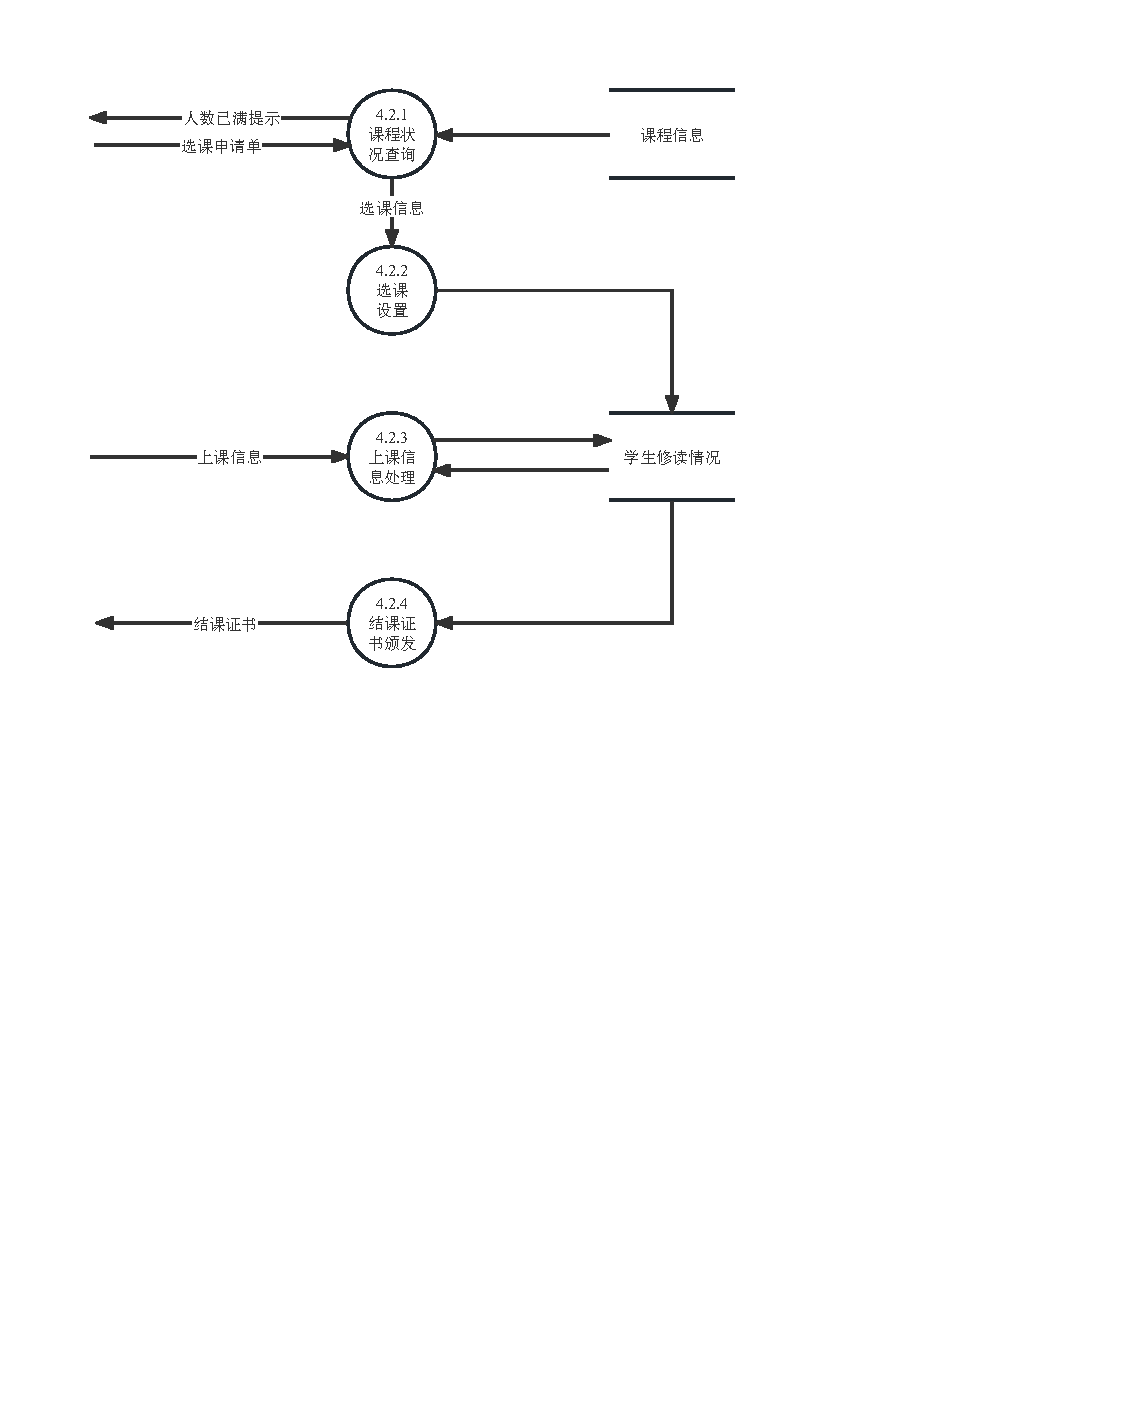
\includegraphics[width=0.95\textwidth]  {fig/课程管理/C_2-2.pdf}} 
    \bicaption{公益课程系统2层数据流图}{Data Flow Diagram for Level 2 of Public Course System}
    \end{figure}
    
(1)数据加工词条描述说明
\begin{table}[H]  
\caption{“课程状况查询”加工词条描述}  
\begin{center}  
    \begin{tabular}{l p{11cm}} 
        \hline
        \quad 名称: & 课程状况查询 \\
        \hline
        \quad 编号: & 4.2.1 \\
        \hline
        \quad 简述: & 查询课程状况的功能 \\
        \hline
        \quad 输入: & 选课申请书、课程信息、用户权限 \\
        \hline
        \quad 输出: & 人数已满提示、选课信息 \\
        \hline
        \quad 逻辑: & 指志愿者查询课程信息和课程人数。 \\
        \hline
    \end{tabular}
    \label{tab1}
\end{center}
\end{table}


\begin{algorithm}[H]
    \renewcommand{\thealgorithm}{}
    \caption{“课程状况查询”加工小说明} 
    \label{alg3} 
    \begin{algorithmic}[1]
        \STATE Analyze 课程信息
        \STATE Generate 选课申请书 Based On 用户权限
        \STATE Write 课程状况分析报表字段 To 选课信息
    \end{algorithmic} 
\end{algorithm}

\begin{table}[H]  
\caption{“选课设置”加工词条描述}  
\begin{center}  
    \begin{tabular}{l p{11cm}} 
        \hline
        \quad 名称: & 选课设置 \\
        \hline
        \quad 编号: & 4.2.2 \\
        \hline
        \quad 简述: & 设置学生选课情况的功能 \\
        \hline
        \quad 输入: & 选课设置、课程信息\\
        \hline
        \quad 输出: & 学生修读情况 \\
        \hline
        \quad 逻辑: & 为志愿者提供不同课程选择和设置,同时导入课程信息。 \\
        \hline
    \end{tabular}
    \label{tab1}
\end{center}
\end{table}


\begin{algorithm}[H]
    \renewcommand{\thealgorithm}{}
    \caption{“选课设置”加工小说明} 
    \label{alg3} 
    \begin{algorithmic}[1]
        \STATE Get 课程名 + 课程类别 From 可选课程信息
        \STATE Insert 课程名 + 课程类别 Into 学生修读情况
    \end{algorithmic} 
\end{algorithm}



\begin{table}[H]  
\caption{“上课信息处理”加工词条描述}  
\begin{center}  
    \begin{tabular}{l p{11cm}} 
        \hline
        \quad 名称: & 上课信息处理 \\
        \hline
        \quad 编号: & 4.2.3 \\
        \hline
        \quad 简述: & 处理学生上课信息的功能 \\
        \hline
        \quad 输入: & 上课信息、学生修读情况 \\
        \hline
        \quad 输出: & 学生修读情况 \\
        \hline
        \quad 逻辑: & 通过在线方式获取、记录、整理和分析志愿者的学习情况和表现。 \\
        \hline
    \end{tabular}
    \label{tab1}
\end{center}
\end{table}


\begin{algorithm}[H]
    \renewcommand{\thealgorithm}{}
    \caption{“上课信息处理”加工小说明} 
    \label{alg3} 
    \begin{algorithmic}[1]
        \STATE Select Items In 课程状况 Match 用户ID
        \STATE Write 用户ID, 课程修读情况, 消息内容 To 学生修读情况
    \end{algorithmic} 
\end{algorithm}

\begin{table}[H]  
\caption{“结课证书颁发”加工词条描述}  
\begin{center}  
    \begin{tabular}{l p{11cm}} 
        \hline
        \quad 名称: & 结课证书颁发 \\
        \hline
        \quad 编号: & 4.2.4 \\
        \hline
        \quad 简述: & 给志愿者颁发结课证书的功能 \\
        \hline
        \quad 输入: & 学生修读情况 \\
        \hline
        \quad 输出: & 结课证书 \\
        \hline
        \quad 逻辑: & 完成一定的课程学习后,由相关机构颁发证书,证明志愿者完成该课程学习。 \\
        \hline
    \end{tabular}
    \label{tab1}
\end{center}
\end{table}


\begin{algorithm}[H]
    \renewcommand{\thealgorithm}{}
    \caption{“结课证书颁发”加工小说明} 
    \label{alg3} 
    \begin{algorithmic}[1]
        \STATE Create 结课证书ID
        \STATE Get 系统时间 As 颁发时间
        \STATE Set 课程名 + 用户ID As 证书信息
        \STATE Write 颁发时间 + 证书信息 To 结课证书
    \end{algorithmic} 
\end{algorithm}

(2)数据流词条描述说明
\begin{table}[H]  
\caption{``授课申请书"数据流词条描述}  
\begin{center}  
    \begin{tabular}{l p{11cm}} 
        \hline
        \quad 名称: & 授课申请书 \\
        \hline
        \quad 简述: & 授课人对授课的申请 \\
        \hline
        \quad 来源: & 源点``授课人" \\
        \hline
        \quad 去向: & 加工``登录状态查询" \\
        \hline
        \quad 组成: & 授课申请书+用户ID+用户密码 \\
        \hline
    \end{tabular}
    \label{tab1}
\end{center}
\end{table}

\begin{table}[H]  
\caption{``权限不足提示"数据流词条描述}  
\begin{center}  
    \begin{tabular}{l p{11cm}} 
        \hline
        \quad 名称: & 权限不足提示 \\
        \hline
        \quad 简述: & 查询登录状态的结果 \\
        \hline
        \quad 来源: & 加工``登录状态查询" \\
        \hline
        \quad 去向: & 源点``授课人" \\
        \hline
        \quad 组成: & 登录状态+用户ID+用户名+权限信息 \\
        \hline
    \end{tabular}
    \label{tab1}
\end{center}
\end{table}


\begin{table}[H]  
\caption{``申请通过提示"数据流词条描述}  
\begin{center}  
    \begin{tabular}{l p{11cm}} 
        \hline
        \quad 名称: & 申请通过提示 \\
        \hline
        \quad 简述: & 授课申请处理的结果 \\
        \hline
        \quad 来源: & 加工``授课申请处理" \\
        \hline
        \quad 去向: & 源点``授课人" \\
        \hline
        \quad 组成: & 用户名+用户ID+用户权限+授课申请书编号+申请处理信息+申请处理时间 \\
        \hline
    \end{tabular}
    \label{tab1}
\end{center}
\end{table}


\begin{table}[H]  
\caption{``课程信息"数据流词条描述}  
\begin{center}  
    \begin{tabular}{l p{11cm}} 
        \hline
        \quad 名称: & 课程信息 \\
        \hline
        \quad 简述: & 申请通过的课程的信息 \\
        \hline
        \quad 来源: & 加工``授课申请处理" \\
        \hline
        \quad 去向: & 加工``课程内容设置" \\
        \hline
        \quad 组成: & 课程ID+课程名+用户ID+用户权限+课程内容+课程资料+课程收费 \\
        \hline
    \end{tabular}
    \label{tab1}
\end{center}
\end{table}



\begin{table}[H]  
\caption{``课程信息修改单"数据流词条描述}  
\begin{center}  
    \begin{tabular}{l p{11cm}} 
        \hline
        \quad 名称: & 课程信息修改单 \\
        \hline
        \quad 简述: & 授课人对课程修改的信息 \\
        \hline
        \quad 来源: & 源点``授课人" \\
        \hline
        \quad 去向: & 加工``课程内容修改" \\
        \hline
        \quad 组成: & 课程ID+课程名+用户ID+用户权限+用户密码+课程内容+课程资料+课程收费 \\
        \hline
    \end{tabular}
    \label{tab1}
\end{center}
\end{table}

\begin{table}[H]  
\caption{``授课证书"数据流词条描述}  
\begin{center}  
    \begin{tabular}{l p{11cm}} 
        \hline
        \quad 名称: & 授课证书 \\
        \hline
        \quad 简述: & 颁发的授课证书信息 \\
        \hline
        \quad 来源: & 加工``授课证书颁发" \\
        \hline
        \quad 去向: & 源点``授课人" \\
        \hline
        \quad 组成: & 课程ID+课程名+用户ID+用户名+课程内容+课程证书 \\
        \hline
    \end{tabular}
    \label{tab1}
\end{center}
\end{table}



\begin{table}[H]  
\caption{``修读情况分析"数据流词条描述}  
\begin{center}  
    \begin{tabular}{l p{11cm}} 
        \hline
        \quad 名称: & 修读情况分析 \\
        \hline
        \quad 简述: & 学生的修读情况分析 \\
        \hline
        \quad 来源: & 加工``学生上课情况分析" \\
        \hline
        \quad 去向: & 源点``志愿者" \\
        \hline
        \quad 组成: & 用户ID+用户权限+用户名+学习课程+授课人名+考核情况+课程进度+学习课程反馈+学习课程数量 \\
        \hline
    \end{tabular}
    \label{tab1}
\end{center}
\end{table}



(3)文件词条描述
\begin{table}[H]  
\caption{“已登录用户权限表”文件词条描述}  
\begin{center}  
    \begin{tabular}{l p{10cm}} 
        \hline
        \quad 名称: & 已登录用户权限表 \\
        \hline
        \quad 简述: & 存储已登录用户权限\\
        \hline
        \quad 组成: & 用户ID+用户账号+用户名+用户密码+用户邮箱地址+用户权限 \\
        \hline
        \quad 存储方式: & 以用户ID为关键字。 \\
        \hline
    \end{tabular}
    \label{tab1}
\end{center}
\end{table}

\begin{table}[H]  
\caption{“课程信息”文件词条描述}  
\begin{center}  
    \begin{tabular}{l p{10cm}} 
        \hline
        \quad 名称: & 课程信息 \\
        \hline
        \quad 简述: & 存储课程信息 \\
        \hline
        \quad 组成: & 课程ID+课程名+用户ID+用户名+用户权限+课程内容+课程进度+课程资料+课程收费+课程人数 \\
        \hline
        \quad 存储方式: & 以课程ID为关键字。 \\
        \hline
    \end{tabular}
    \label{tab1}
\end{center}
\end{table}

\begin{table}[H]  
\caption{“学生修读情况”文件词条描述}  
\begin{center}  
    \begin{tabular}{l p{10cm}} 
        \hline
        \quad 名称: & 学生修读情况 \\
        \hline
        \quad 简述: & 存储学生修读情况 \\
        \hline
        \quad 组成: & 用户ID+用户权限+用户名+学习课程+授课人ID+授课人名+授课人权限+考核情况+课程进度+学习课程反馈+学习课程数量  \\
        \hline
        \quad 存储方式: & 以用户ID为关键字。 \\
        \hline
    \end{tabular}
    \label{tab1}
\end{center}
\end{table}


\paragraph{反馈管理}~{}
\\

\begin{figure}[H]
    \center{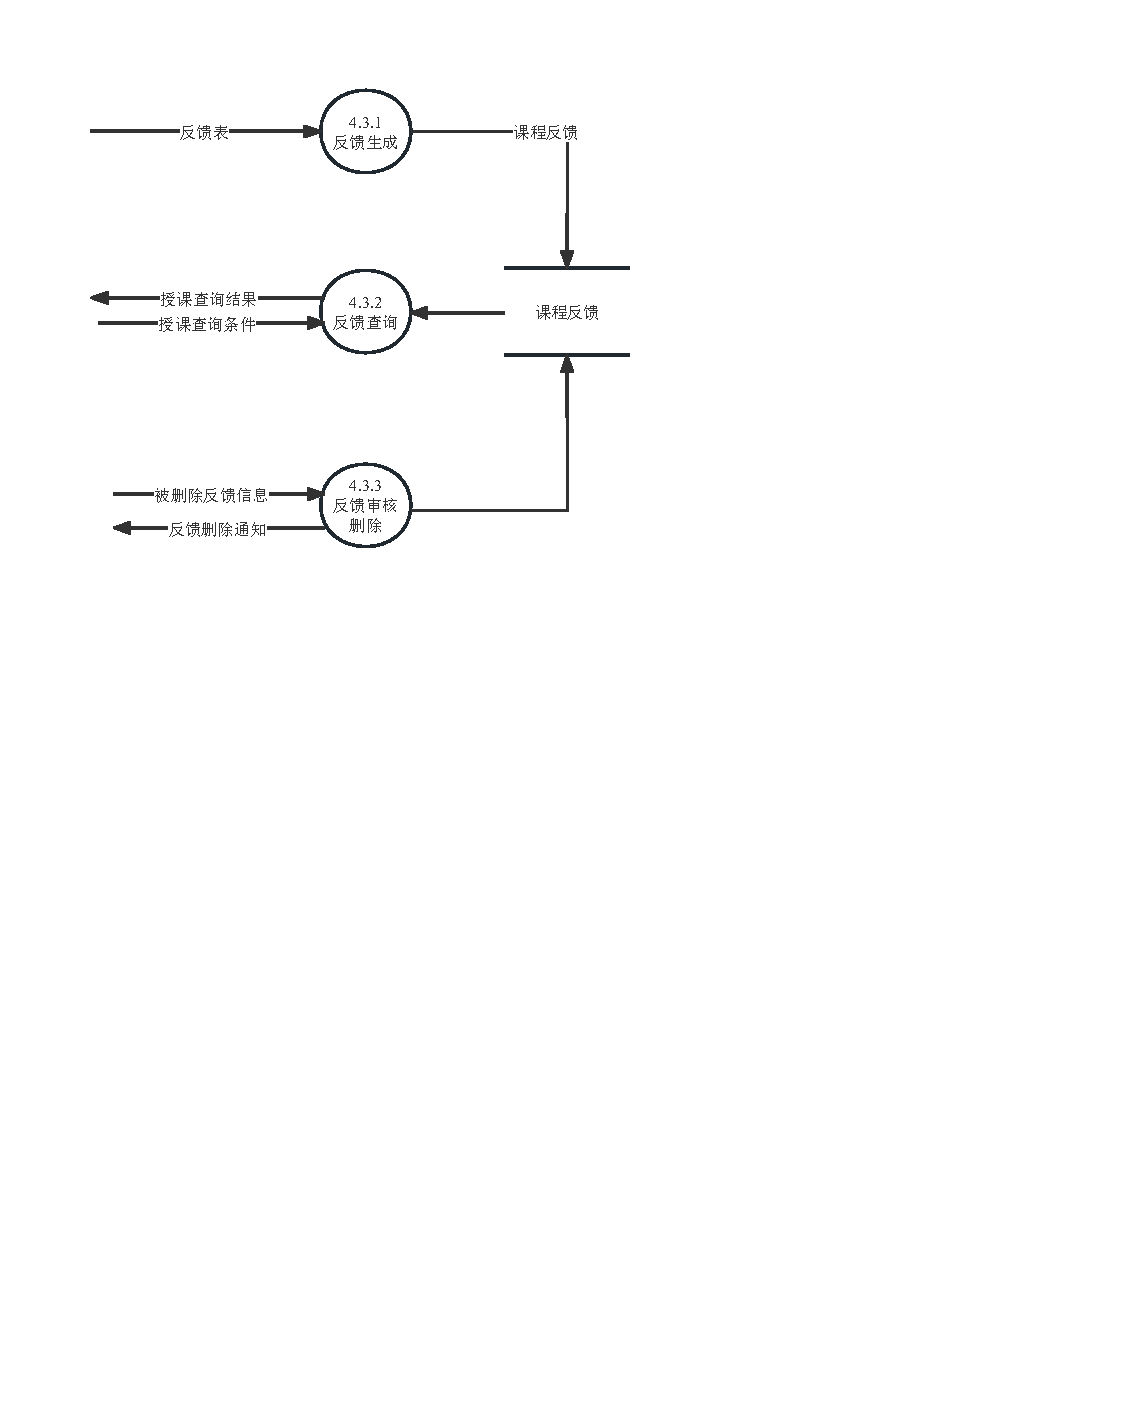
\includegraphics[width=0.95\textwidth]  {fig/课程管理/C_2-3.pdf}} 
    \bicaption{公益课程系统2层数据流图}{Data Flow Diagram for Level 2 of Public Course System}
    \end{figure}
    
(1)数据加工词条描述说明
\begin{table}[H]  
\caption{“反馈生成”加工词条描述}  
\begin{center}  
    \begin{tabular}{l p{11cm}} 
        \hline
        \quad 名称: & 反馈生成 \\
        \hline
        \quad 编号: & 4.3.1 \\
        \hline
        \quad 简述: & 生成反馈信息的功能 \\
        \hline
        \quad 输入: & 反馈表 \\
        \hline
        \quad 输出: & 课程反馈 \\
        \hline
        \quad 逻辑: & 将生成的反馈描述整理成一个文档或报告,以便课程组织者和授课人参考。 \\
        \hline
    \end{tabular}
    \label{tab1}
\end{center}
\end{table}


\begin{algorithm}[H]
    \renewcommand{\thealgorithm}{}
    \caption{“反馈生成”加工小说明} 
    \label{alg3} 
    \begin{algorithmic}[1]
        \STATE Get 系统时间 As 发送时间
        \STATE Generate 反馈ID 
        \STATE Write 反馈发送记录 + 反馈ID + 发送时间 To 课程反馈
    \end{algorithmic} 
\end{algorithm}

\begin{table}[H]  
\caption{“反馈查询”加工词条描述}  
\begin{center}  
    \begin{tabular}{l p{11cm}} 
        \hline
        \quad 名称: & 反馈查询 \\
        \hline
        \quad 编号: & 4.3.2 \\
        \hline
        \quad 简述: & 授课人进行反馈查询的功能 \\
        \hline
        \quad 输入: & 查询条件、课程反馈 \\
        \hline
        \quad 输出: & 查询结果 \\
        \hline
        \quad 逻辑: & 授课人选择条件查询自己教授课程,得到回应或解决方案。 \\
        \hline
    \end{tabular}
    \label{tab1}
\end{center}
\end{table}


\begin{algorithm}[H] 
    \renewcommand{\thealgorithm}{}
    \caption{“反馈查询”加工小说明} 
    \label{alg3} 
    \begin{algorithmic}[1]
        \STATE Get 系统时间 As 查询时间
        \STATE Write 查询条件 + 课程反馈 To 查询结果 
    \end{algorithmic} 
\end{algorithm}

\begin{table}[H]  
\caption{“反馈审核删除”加工词条描述}  
\begin{center}  
    \begin{tabular}{l p{11cm}} 
        \hline
        \quad 名称: & 反馈审核删除 \\
        \hline
        \quad 编号: & 4.3.3 \\
        \hline
        \quad 简述: & 系统管理员进行反馈审核删除的功能 \\
        \hline
        \quad 输入: & 被删除反馈信息 \\
        \hline
        \quad 输出: & 课程反馈、反馈删除通知 \\
        \hline
        \quad 逻辑: & 管理员对已经发布的反馈信息进行审核,判断其是否违反了相关规定或政策,并在必要时将其删除。 \\
        \hline
    \end{tabular}
    \label{tab1}
\end{center}
\end{table}


\begin{algorithm}[H]
    \renewcommand{\thealgorithm}{}
    \caption{“反馈审核删除”加工小说明} 
    \label{alg3} 
    \begin{algorithmic}[1]
        \STATE Select Items In 反馈 Match 反馈审核
        \STATE Delete 用户ID, 反馈内容 To 课程反馈
    \end{algorithmic} 
\end{algorithm}

(2)数据流词条描述说明
\begin{table}[H]  
\caption{``反馈表"数据流词条描述}  
\begin{center}  
    \begin{tabular}{l p{11cm}} 
        \hline
        \quad 名称: & 反馈表 \\
        \hline
        \quad 简述:  & 志愿者对课程反馈的信息 \\
        \hline
        \quad 来源:  & 源点``志愿者" \\
        \hline
        \quad 去向:  & 加工``反馈生成" \\
        \hline
        \quad 组成:  & 用户反馈ID+用户反馈信息+用户ID+用户名+课程ID+课程名+授课人名+反馈表提交时间 \\
        \hline
    \end{tabular}
    \label{tab1}
\end{center}
\end{table}


\begin{table}[H]  
\caption{``授课查询结果"数据流词条描述}  
\begin{center}  
    \begin{tabular}{l p{11cm}} 
        \hline
        \quad 名称: & 授课查询结果 \\
        \hline
        \quad 简述:  & 授课人对课程的查询结果 \\
        \hline
        \quad 来源:  & 加工``反馈查询" \\
        \hline
        \quad 去向:  & 源点``授课人" \\
        \hline
        \quad 组成:  & 用户反馈ID+用户反馈信息+课程ID+课程名+课程内容  \\
        \hline
    \end{tabular}
    \label{tab1}
\end{center}
\end{table}

\begin{table}[H]  
\caption{``授课查询条件"数据流词条描述}  
\begin{center}  
    \begin{tabular}{l p{11cm}} 
        \hline
        \quad 名称: & 授课查询条件 \\
        \hline
        \quad 简述: & 授课人对课程的查询条件 \\
        \hline
        \quad 来源: & 源点``授课人" \\
        \hline
        \quad 去向: & 加工``反馈查询" \\
        \hline
        \quad 组成: & 课程ID+课程名+课程内容+授课人ID+授课人名+查询时间  \\
        \hline
    \end{tabular}
    \label{tab1}
\end{center}
\end{table}

\begin{table}[H]  
\caption{``被删除反馈信息"数据流词条描述}  
\begin{center}  
    \begin{tabular}{l p{11cm}} 
        \hline
        \quad 名称: & 被删除反馈信息 \\
        \hline
        \quad 简述: & 被系统管理员删除的反馈信息 \\
        \hline
        \quad 来源: & 源点``系统管理员" \\
        \hline
        \quad 去向: & 加工``反馈审核删除"\\
        \hline
        \quad 组成: & 审核删除原因+审核删除条规+审核删除时间+用户反馈ID+用户反馈信息  \\
        \hline
    \end{tabular}
    \label{tab1}
\end{center}
\end{table}

\begin{table}[H]  
\caption{``反馈删除通知"数据流词条描述}  
\begin{center}  
    \begin{tabular}{l p{11cm}} 
        \hline
        \quad 名称: & 反馈删除通知 \\
        \hline
        \quad 简述: & 发给志愿者的反馈删除通知 \\
        \hline
        \quad 来源: & 加工``反馈审核删除" \\
        \hline
        \quad 去向: & 源点``志愿者" \\
        \hline
        \quad 组成: & 用户反馈ID+用户反馈信息+用户ID+用户名+审核删除原因+审核删除条规+审核删除时间 \\
        \hline
    \end{tabular}
    \label{tab1}
\end{center}
\end{table}



(3)文件词条描述
\begin{table}[H]  
\caption{“课程反馈”文件词条描述}  
\begin{center}  
    \begin{tabular}{l p{10cm}} 
        \hline
        \quad 名称: & 课程反馈 \\
        \hline
        \quad 简述: & 存储课程反馈内容\\
        \hline
        \quad 组成: & 用户反馈ID+用户反馈信息+用户ID+用户名+用户考核情况+课程ID+课程名+课程内容+授课人ID+授课人名 \\
        \hline
        \quad 存储方式: & 以资讯ID为关键字。 \\
        \hline
    \end{tabular}
    \label{tab1}
\end{center}
\end{table}



\paragraph{证书管理}~{}
\\
\begin{figure}[H]
    \center{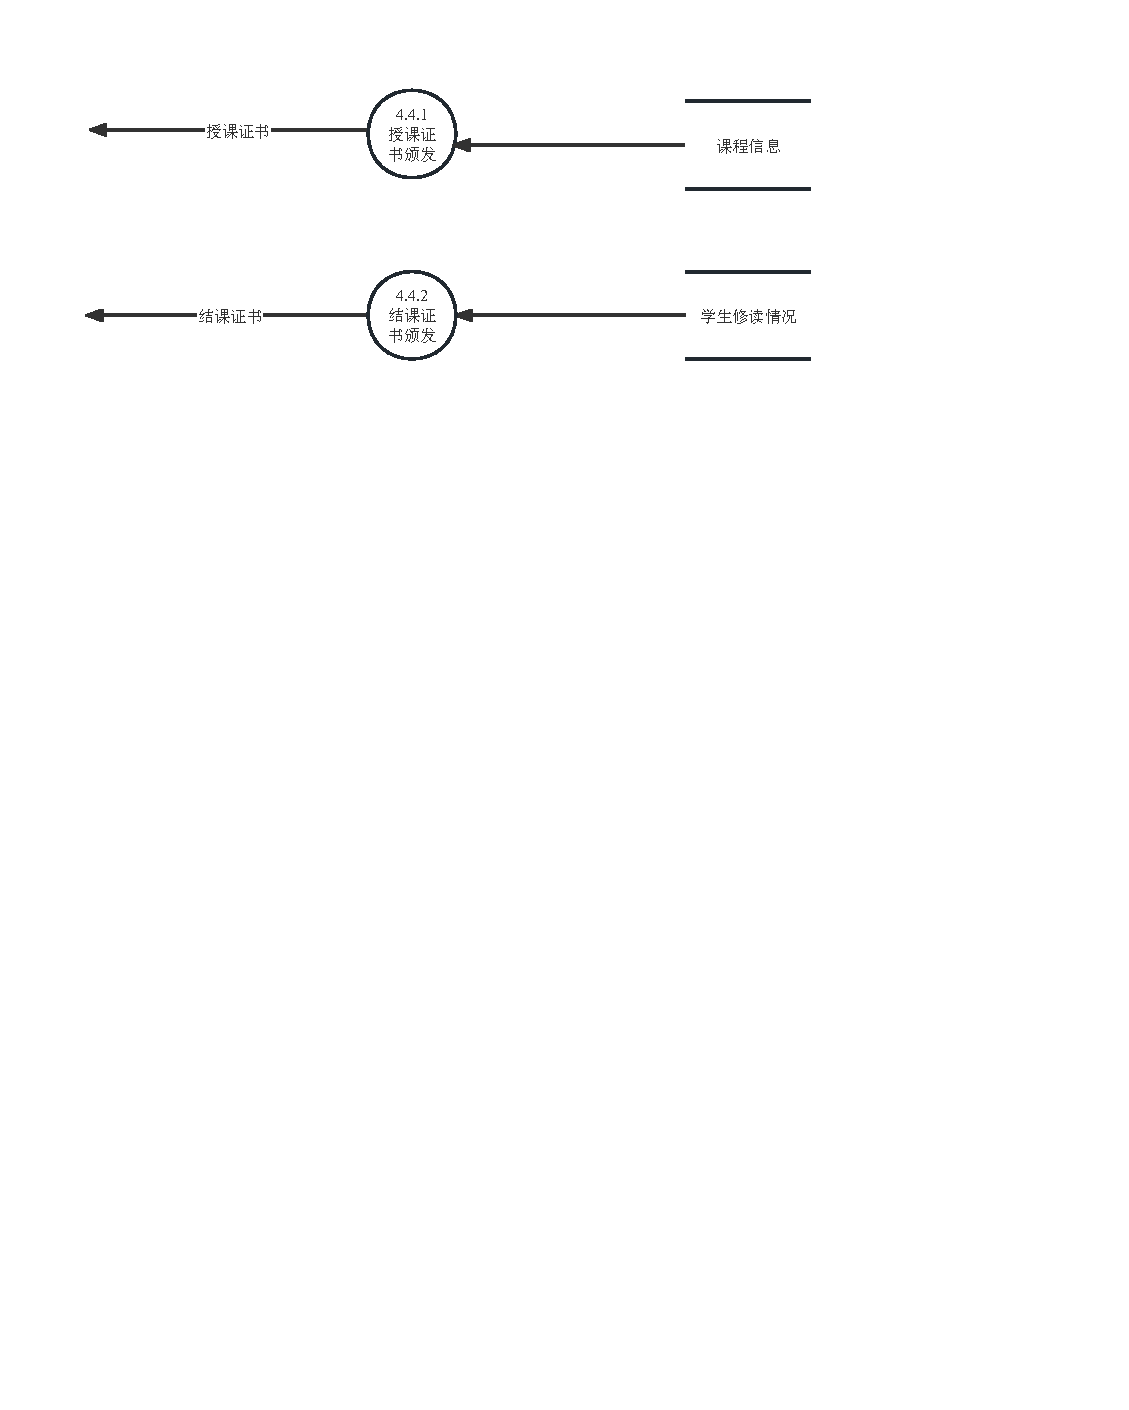
\includegraphics[width=0.95\textwidth]  {fig/课程管理/C_2-4.pdf}} 
    \bicaption{公益课程系统2层数据流图}{Data Flow Diagram for Level 2 of Public Course System}
    \end{figure}
    
(1)数据加工词条描述说明
\begin{table}[H]  
\caption{“授课证书颁发”加工词条描述}  
\begin{center}  
    \begin{tabular}{l p{11cm}} 
        \hline
        \quad 名称: & 授课证书颁发 \\
        \hline
        \quad 编号:  & 4.4.1 \\
        \hline
        \quad 简述:  & 颁发授课证书的功能 \\
        \hline
        \quad 输入:  & 课程信息 \\
        \hline
        \quad 输出:  & 授课证书 \\
        \hline
        \quad 逻辑:  & 由相关机构颁发给授课人的证明授课能力和教学水平的证书。 \\
        \hline
    \end{tabular}
    \label{tab1}
\end{center}
\end{table}

\begin{algorithm}[H]
    \renewcommand{\thealgorithm}{}
    \caption{“授课证书颁发”加工小说明} 
    \label{alg3} 
    \begin{algorithmic}[1]
        \STATE Analyze 授课资质
        \STATE Generate 授课人要求条件 Based On 授课人信息
        \STATE Write 授课准许 To 授课证书
    \end{algorithmic} 
\end{algorithm}

\begin{table}[H]  
\caption{“结课证书颁发”加工词条描述}  
\begin{center}  
    \begin{tabular}{l p{11cm}} 
        \hline
        \quad 名称:  &  结课证书颁发 \\
        \hline
        \quad 编号:  & 4.4.2 \\
        \hline
        \quad 简述:  & 给志愿者颁发结课证书的功能  \\
        \hline
        \quad 输入:  & 学生修读情况 \\
        \hline
        \quad 输出:  & 结课证书 \\
        \hline
        \quad 逻辑:  & 完成一定的课程学习后,由相关机构颁发证书,证明志愿者完成该课程学习。 \\
        \hline
    \end{tabular}
    \label{tab1}
\end{center}
\end{table}

\begin{algorithm}[H]
    \renewcommand{\thealgorithm}{}
    \caption{“结课证书颁发”加工小说明} 
    \label{alg3} 
    \begin{algorithmic}[1]
        \STATE Analyze 学生修读情况
        \STATE Generate 课程测试成绩 Based On 课程信息
        \STATE Write 结课认证 To 结课证书
    \end{algorithmic} 
\end{algorithm}

(2)数据流词条描述说明
\begin{table}[H]  
\caption{``授课证书"数据流词条描述}  
\begin{center}  
    \begin{tabular}{l p{11cm}}
        \hline
        \quad 名称:   & 授课证书 \\
        \hline
        \quad 简述:  & 给授课人颁发的授课证书 \\
        \hline
        \quad 来源:  & 加工``授课证书颁发" \\
        \hline
        \quad 去向:  & 源点``授课人" \\
        \hline
        \quad 组成:  & 课程ID+课程名+用户ID+用户名+课程内容+课程证书 \\
        \hline
    \end{tabular}
    \label{tab1}
\end{center}
\end{table}

\begin{table}[H]  
\caption{``结课证书"数据流词条描述}  
\begin{center}  
    \begin{tabular}{l p{11cm}} 
        \hline
        \quad 名称:    & 结课证书 \\
        \hline
        \quad 简述:  & 给志愿者颁发的结课证书 \\
        \hline
        \quad 来源:  & 加工``结课证书" \\
        \hline
        \quad 去向:  & 源点``志愿者" \\
        \hline
        \quad 组成:  &  用户ID+用户名+学习课程+授课人ID+授课人名+考核情况 \\
        \hline
    \end{tabular}
    \label{tab1}
\end{center}
\end{table}

(3)文件词条描述


\subsubsection{交流论坛系统}
以下是交流论坛系统的 1 层数据流图、加工子图以及对应的数据字典和文件。

\begin{figure}[H]
    \center{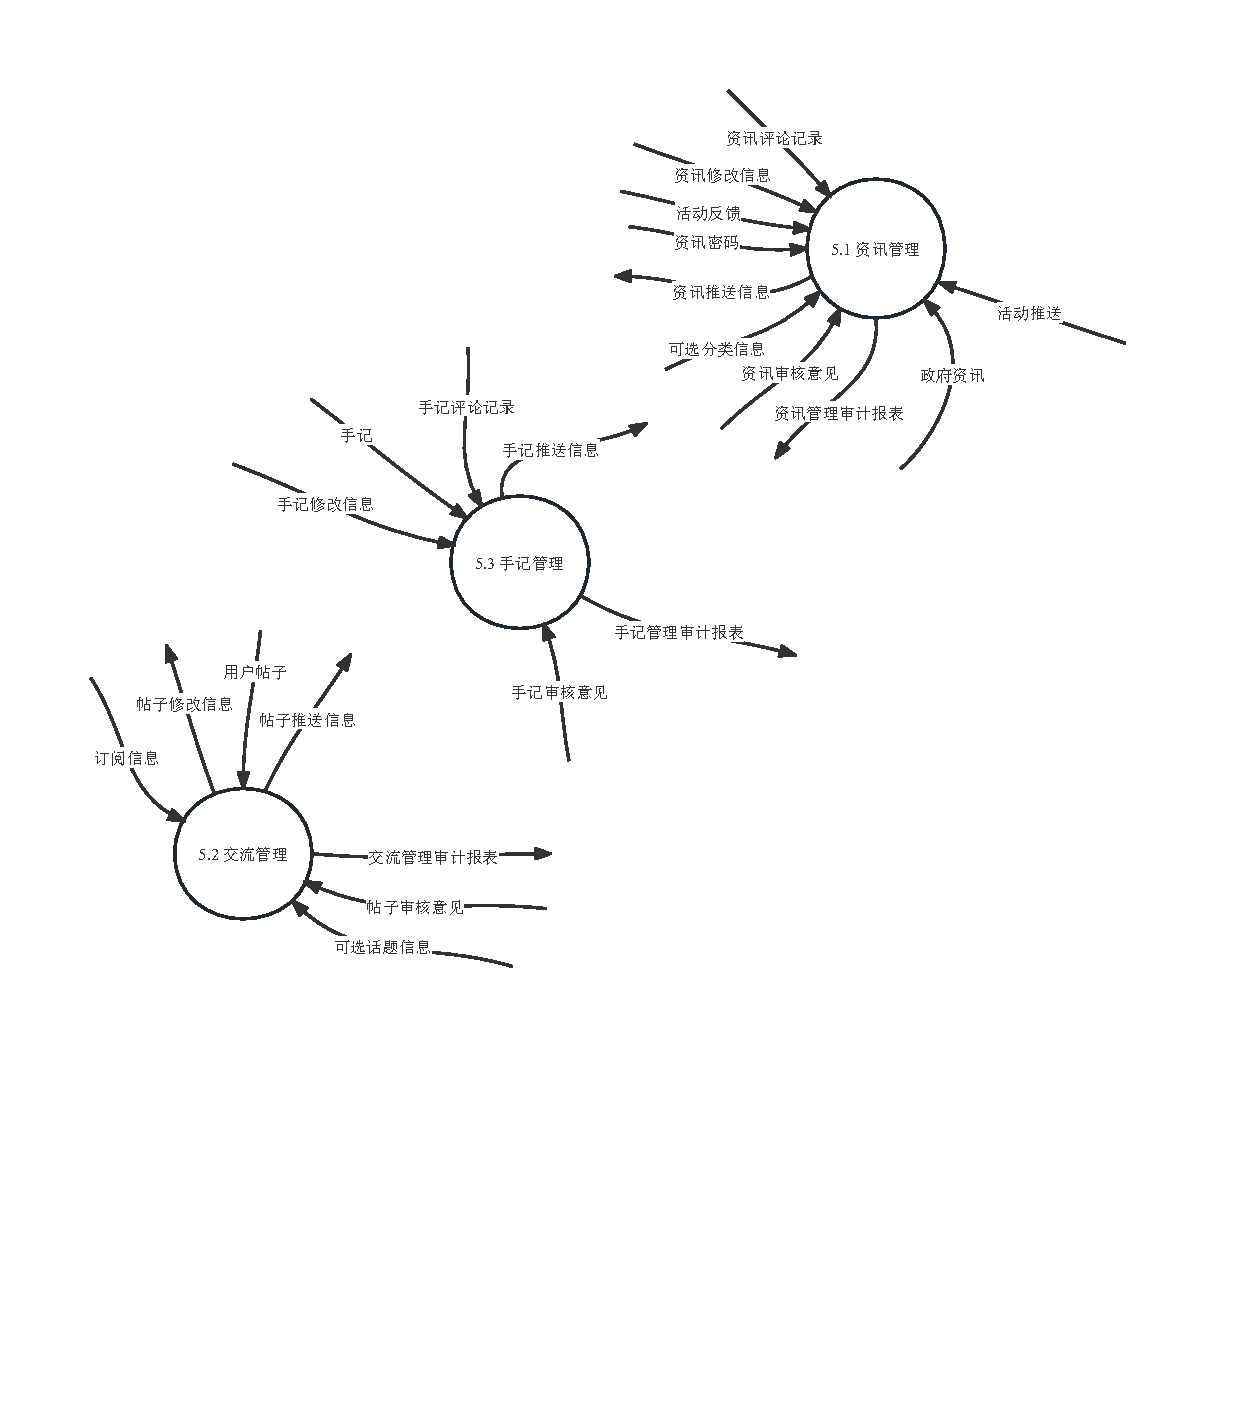
\includegraphics[width=0.95\textwidth]  {fig/论坛管理/F_1.pdf}} 
    \bicaption{交流论坛系统1层数据流图}{Data Flow Diagram for Level 1 of Communication Forum System}
    \end{figure}
    
\paragraph{资讯管理}~{}
\\
\begin{figure}[H]
    \center{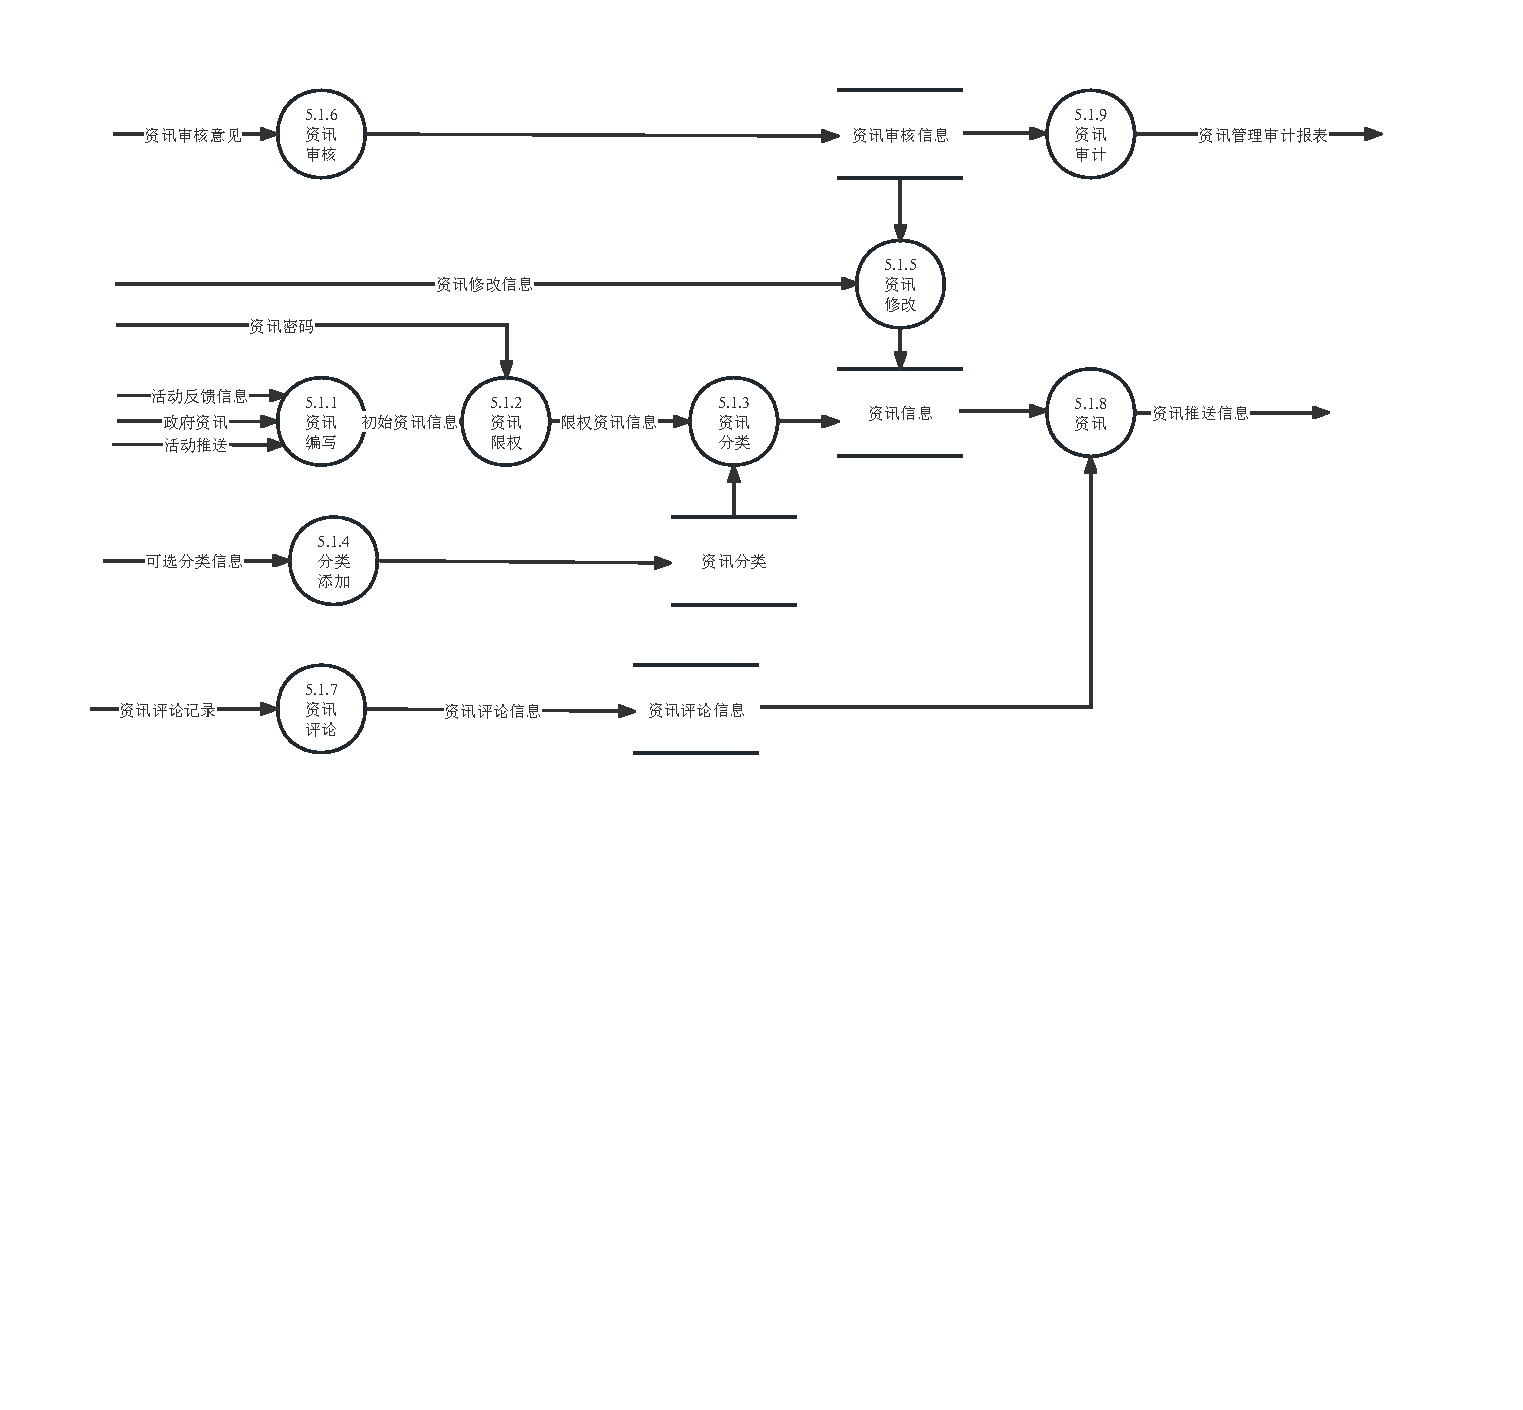
\includegraphics[width=0.95\textwidth]  {fig/论坛管理/F_2-1.pdf}} 
    \bicaption{交流论坛系统2层数据流图}{Data Flow Diagram for Level 2 of Communication Forum System}
    \end{figure}
    
(1)数据加工词条描述说明
\begin{table}[H]  
\caption{“资讯编写”加工词条描述}  
\begin{center}  
    \begin{tabular}{l p{11cm}} 
        \hline
        \quad 名称:  & 资讯编写 \\
        \hline
        \quad 编号:  & 5.1.1 \\
        \hline
        \quad 简述:  & 资讯编写的功能 \\
        \hline
        \quad 输入:  & 活动反馈信息、政府资讯、活动推送信息 \\
        \hline
        \quad 输出:  & 资讯信息 \\
        \hline
        \quad 逻辑:  & 保存用户资讯的内容信息。 \\
        \hline
    \end{tabular}
    \label{tab1}
\end{center}
\end{table}

\begin{algorithm}[H]
    \renewcommand{\thealgorithm}{}
    \caption{“资讯编写”加工小说明} 
    \label{alg3} 
    \begin{algorithmic}[1]
        \STATE Create 资讯ID
        \STATE Get 系统时间 As 发布时间
        \STATE Set 最后编辑时间 As 发布时间
        \STATE Write [活动反馈信息|活动推动信息|官方资讯信息] + 资讯ID + 发布时间 +最后编辑时间 To 初始资讯信息
    \end{algorithmic} 
\end{algorithm}

\begin{table}[H]  
\caption{“资讯限权”加工词条描述}  
\begin{center}  
    \begin{tabular}{l p{11cm}} 
        \hline
        \quad 名称:  &  资讯限权 \\
        \hline
        \quad 编号:  & 5.1.2 \\
        \hline
        \quad 简述:  & 用户设置资讯阅读权限的功能 \\
        \hline
        \quad 输入:  & 资讯密码 \\
        \hline
        \quad 输出:  & 限权资讯信息 \\
        \hline
        \quad 逻辑:  & 用户如需给资讯设置密码,可以给出资讯密码信息。 \\
        \hline
    \end{tabular}
    \label{tab1}
\end{center}
\end{table}

\begin{algorithm}[H]
    \renewcommand{\thealgorithm}{}
    \caption{“资讯限权”加工小说明} 
    \label{alg3} 
    \begin{algorithmic}[1]
        \IF{ Get 资讯密码}
        \STATE Write 初始资讯信息 + 资讯密码 To 限权资讯信息
        \ELSE
        \STATE Write 初始资讯信息 To 限权资讯信息
        \ENDIF
    \end{algorithmic} 
\end{algorithm}


\begin{table}[H]  
\caption{“资讯分类”加工词条描述}  
\begin{center}  
    \begin{tabular}{l p{11cm}} 
        \hline
        \quad 名称:  &  资讯分类 \\
        \hline
        \quad 编号:  & 5.1.3 \\
        \hline
        \quad 简述:  & 用户选择资讯分类的功能 \\
        \hline
        \quad 输入:  & 限权资讯信息、资讯分类信息 \\
        \hline
        \quad 输出:  & 资讯信息 \\
        \hline
        \quad 逻辑:  & 根据资讯分类、限权资讯信息生成资讯信息。 \\
        \hline
    \end{tabular}
    \label{tab1}
\end{center}
\end{table}

\begin{algorithm}[H]
    \renewcommand{\thealgorithm}{}
    \caption{“资讯分类”加工小说明} 
    \label{alg3} 
    \begin{algorithmic}[1]
        \STATE Generate 类别ID + 资讯类别 Based On 限权资讯信息
        \STATE Write 限权资讯信息 + 类别ID + 资讯类别 To 资讯信息
    \end{algorithmic} 
\end{algorithm}

\begin{table}[H]  
\caption{“分类设置”加工词条描述}  
\begin{center}  
    \begin{tabular}{l p{11cm}} 
        \hline
        \quad 名称:  & 资讯设置 \\
        \hline
        \quad 编号:  & 5.1.4\\
        \hline
        \quad 简述:  & 系统管理员设置好资讯分类的功能 \\
        \hline
        \quad 输入:  & 可选分类信息 \\
        \hline
        \quad 输出:  & 资讯分类 \\
        \hline
        \quad 逻辑:  & 根据可选分类信息生成资讯分类。 \\
        \hline
    \end{tabular}
    \label{tab1}
\end{center}
\end{table}

\begin{algorithm}[H]
    \renewcommand{\thealgorithm}{}
    \caption{“分类设置”加工小说明} 
    \label{alg3} 
    \begin{algorithmic}[1]
        \STATE Get 类别ID + 资讯类别 From 可选分类信息
        \STATE Insert 类别ID + 资讯类别 Into 资讯分类
    \end{algorithmic} 
\end{algorithm}

\begin{table}[H]  
\caption{“资讯修改”加工词条描述}  
\begin{center}  
    \begin{tabular}{l p{11cm}} 
        \hline
        \quad 名称:  & 资讯修改 \\
        \hline
        \quad 编号:  & 5.1.5 \\
        \hline
        \quad 简述:  & 对资讯进行修改的功能 \\
        \hline
        \quad 输入:  & 资讯修改信息、资讯审核意见 \\
        \hline
        \quad 输出:  & 资讯信息 \\
        \hline
        \quad 逻辑:  & 完成用户修改资讯的处理。 \\
        \hline
    \end{tabular}
    \label{tab1}
\end{center}
\end{table}

\begin{algorithm}[H] 
    \renewcommand{\thealgorithm}{}
    \caption{“资讯修改”加工小说明} 
    \label{alg3} 
    \begin{algorithmic}[1]
        \STATE Get 资讯ID From 资讯修改信息
        \STATE Update Item In 资讯信息 Match 资讯ID With 资讯修改信息
    \end{algorithmic} 
\end{algorithm}

\begin{table}[H]  
\caption{“资讯审核”加工词条描述}  
\begin{center}  
    \begin{tabular}{l p{11cm}} 
        \hline
        \quad 名称:  &  资讯审核 \\
        \hline
        \quad 编号:  & 5.1.6 \\
        \hline
        \quad 简述:  & 系统管理员审核资讯的功能 \\
        \hline
        \quad 输入:  & 资讯审核意见 \\
        \hline
        \quad 输出:  & 资讯审核信息 \\
        \hline
        \quad 逻辑:  & 系统管理员审核资讯信息,并给出资讯的修改要求。 \\
        \hline
    \end{tabular}
    \label{tab1}
\end{center}
\end{table}

\begin{algorithm}[H]
    \renewcommand{\thealgorithm}{}
    \caption{“资讯审核”加工小说明} 
    \label{alg3} 
    \begin{algorithmic}[1]
        \STATE Get 系统时间 As 审核时间
        \STATE Write 资讯审核意见 + 审核时间 To 资讯审核信息
    \end{algorithmic} 
\end{algorithm}

\begin{table}[H]  
\caption{“资讯评论”加工词条描述}  
\begin{center}  
    \begin{tabular}{l p{11cm}} 
        \hline
        \quad 名称:  &  资讯评论 \\
        \hline
        \quad 编号:  & 5.1.7 \\
        \hline
        \quad 简述:  & 对资讯进行评论的功能 \\
        \hline
        \quad 输入:  & 资讯评论记录 \\
        \hline
        \quad 输出:  & 资讯评论信息 \\
        \hline
        \quad 逻辑:  & 用户给出对资讯的评论。 \\
        \hline
    \end{tabular}
    \label{tab1}
\end{center}
\end{table}

\begin{algorithm}[H]
    \renewcommand{\thealgorithm}{}
    \caption{“资讯评论”加工小说明} 
    \label{alg3} 
    \begin{algorithmic}[1]
        \STATE Create 评论ID
        \STATE Get 系统时间 As 提交时间
        \STATE Write 资讯评论记录+评论ID+提交时间+资讯评论信息
    \end{algorithmic} 
\end{algorithm}

\begin{table}[H]  
\caption{“资讯推送”加工词条描述}  
\begin{center}  
    \begin{tabular}{l p{11cm}} 
        \hline
        \quad 名称:  & 资讯推送 \\
        \hline
        \quad 编号:  & 5.1.8 \\
        \hline
        \quad 简述:  & 资讯推送的功能 \\
        \hline
        \quad 输入:  & 资讯信息 \\
        \hline
        \quad 输出:  & 推送信息 \\
        \hline
        \quad 逻辑:  & 根据资讯信息筛选出热度较高的手记推送信息。 \\
        \hline
    \end{tabular}
    \label{tab1}
\end{center}
\end{table}

\begin{algorithm}[H]
    \renewcommand{\thealgorithm}{}
    \caption{“资讯推送”加工小说明} 
    \label{alg3} 
    \begin{algorithmic}[1]
        \STATE Analyze In 资讯信息
        \STATE Get 资讯ID From 资讯信息
        \STATE Select 对应资讯评论 From 资讯评论信息 Match 资讯ID
        \STATE Write 资讯信息 + 对应资讯评论 To 资讯推送信息
    \end{algorithmic} 
\end{algorithm}

\begin{table}[H]  
\caption{“资讯审计”加工词条描述}  
\begin{center}  
    \begin{tabular}{l p{11cm}} 
        \hline
        \quad 名称:  & 资讯审计 \\
        \hline
        \quad 编号:  & 5.1.9 \\
        \hline
        \quad 简述:  & 审计资讯的功能 \\
        \hline
        \quad 输入:  & 资讯审核信息 \\
        \hline
        \quad 输出:  & 资讯管理审计报表 \\
        \hline
        \quad 逻辑:  & 根据资讯审核信息分析生成资讯管理审计报表。 \\
        \hline
    \end{tabular}
    \label{tab1}
\end{center}
\end{table}

\begin{algorithm}[H]
    \renewcommand{\thealgorithm}{}
    \caption{“资讯审计”加工小说明} 
    \label{alg3} 
    \begin{algorithmic}[1]
        \STATE Analyze 资讯审核信息
        \STATE Generate 资讯审核信息统计分析报表字段 Based On 资讯审核信息
        \STATE Write 资讯审核信息统计分析报表字段 To 资讯审计报表
    \end{algorithmic} 
\end{algorithm}


(2)数据流词条描述说明
\begin{table}[H]  
\caption{``活动反馈信息"数据流词条描述}  
\begin{center}  
    \begin{tabular}{l p{11cm}} 
        \hline
        \quad 名称:  &  活动反馈信息 \\
        \hline
        \quad 简述:  & 志愿者对活动反馈的信息 \\
        \hline
        \quad 来源:  & 源点``志愿者" \\
        \hline
        \quad 去向:  & 加工``资讯编写" \\
        \hline
        \quad 组成:  & 用户名+用户ID+资讯内容+发布时间+最后编辑时间 \\
        \hline
    \end{tabular}
    \label{tab1}
\end{center}
\end{table}

\begin{table}[H]  
\caption{``活动推送信息"数据流词条描述}  
\begin{center}  
    \begin{tabular}{l p{11cm}} 
        \hline
        \quad 名称:  &  活动推送信息 \\
        \hline
        \quad 简述:  & 志愿团队活动推送的信息 \\
        \hline
        \quad 来源:  & 源点``志愿团队" \\
        \hline
        \quad 去向:  & 加工``资讯编写" \\
        \hline
        \quad 组成:  & 团队ID+团队名+资讯内容+发布时间+最后编辑时间 \\
        \hline
    \end{tabular}
    \label{tab1}
\end{center}
\end{table}

\begin{table}[H]  
\caption{``官方资讯信息"数据流词条描述}  
\begin{center}  
    \begin{tabular}{l p{11cm}} 
        \hline
        \quad 名称:  &  官方资讯信息 \\
        \hline
        \quad 简述:  & 政府机构发布的资讯信息 \\
        \hline
        \quad 来源:  & 源点``政府相关部门" \\
        \hline
        \quad 去向:  & 加工``资讯编写" \\
        \hline
        \quad 组成:  & 政府用户ID+政府机构名+资讯内容+发布时间+最后编辑时间 \\
        \hline
    \end{tabular}
    \label{tab1}
\end{center}
\end{table}

\begin{table}[H]  
\caption{``初始资讯信息"数据流词条描述}  
\begin{center}  
    \begin{tabular}{l p{11cm}} 
        \hline
        \quad 名称:  &  初始资讯信息 \\
        \hline
        \quad 简述:  & 添加新撰写的资讯信息 \\
        \hline
        \quad 来源:  & 加工``资讯编写" \\
        \hline
        \quad 去向:  & 文件``资讯信息" \\
        \hline
        \quad 组成:  & 资讯ID+[用户ID|团队ID|政府用户ID]+[用户名|团队名|政府家机构名]+资讯内容+发布时间+最后编辑时间 \\
        \hline
    \end{tabular}
    \label{tab1}
\end{center}
\end{table}

\begin{table}[H]  
\caption{``限权资讯信息"数据流词条描述}  
\begin{center}  
    \begin{tabular}{l p{11cm}} 
        \hline
        \quad 名称:  &  初始资讯信息 \\
        \hline
        \quad 简述:  & 添加新撰写的资讯信息 \\
        \hline
        \quad 来源:  & 加工``资讯编写" \\
        \hline
        \quad 去向:  & 文件``资讯信息" \\
        \hline
        \quad 组成:  & 资讯ID+用户ID+用户名+资讯内容+{资讯密码}+发布时间+最后编辑时间 \\
        \hline
    \end{tabular}
    \label{tab1}
\end{center}
\end{table}

\begin{table}[H]  
\caption{``可选分类信息"数据流词条描述}  
\begin{center}  
    \begin{tabular}{l p{11cm}} 
        \hline
        \quad 名称:  &  可选分类信息 \\
        \hline
        \quad 简述:  & 可选的资讯分类信息 \\
        \hline
        \quad 来源:  & 源点``系统管理员" \\
        \hline
        \quad 去向:  & 加工``分类设置" \\
        \hline
        \quad 组成:  & 类别ID+类别名称 \\
        \hline
    \end{tabular}
    \label{tab1}
\end{center}
\end{table}

\begin{table}[H]  
\caption{``资讯密码"数据流词条描述}  
\begin{center}  
    \begin{tabular}{l p{11cm}} 
        \hline
        \quad 名称:  &  推送密码 \\
        \hline
        \quad 简述:  & 为活动推送限权的信息 \\
        \hline
        \quad 来源:  & 源点``系统管理员" \\
        \hline
        \quad 去向:  & 加工``资讯限权" \\
        \hline
        \quad 组成:  & 密码 \\
        \hline
    \end{tabular}
    \label{tab1}
\end{center}
\end{table}


\begin{table}[H]  
\caption{``资讯修改信息"数据流词条描述}  
\begin{center}  
    \begin{tabular}{l p{11cm}} 
        \hline
        \quad 名称:  &  资讯修改信息 \\
        \hline
        \quad 简述:  & 修改后的资讯信息 \\
        \hline
        \quad 来源:  & 源点``志愿者" \\
        \hline
        \quad 去想:  & 加工``资讯修改" \\
        \hline
        \quad 组成:  & 用户名+用户ID+资讯名称+编写时间+资讯内容+修改内容+修改说明+提交时间 \\
        \hline
    \end{tabular}
    \label{tab1}
\end{center}
\end{table}

\begin{table}[H]  
\caption{``资讯审核意见"数据流词条描述}  
\begin{center}  
    \begin{tabular}{l p{11cm}} 
        \hline
        \quad 名称:  &  资讯审核意见 \\
        \hline
        \quad 简述:  & 资讯的审核意见 \\
        \hline
        \quad 来源:  & 源点``系统管理员" \\
        \hline
        \quad 去想:  & 加工``资讯审核" \\
        \hline
        \quad 组成:  & 资讯ID+修改要求+审核情况 \\
        \hline
    \end{tabular}
    \label{tab1}
\end{center}
\end{table}

\begin{table}[H]  
\caption{``资讯评论记录"数据流词条描述}  
\begin{center}  
    \begin{tabular}{l p{11cm}} 
        \hline
        \quad 名称:  &  资讯评论记录 \\
        \hline
        \quad 简述:  & 资讯评论的记录信息 \\
        \hline
        \quad 来源:  & 源点``志愿者" \\
        \hline
        \quad 去想:  & 加工``资讯评论" \\
        \hline
        \quad 组成:  & 资讯ID+评论内容+用户ID+用户名 \\
        \hline
    \end{tabular}
    \label{tab1}
\end{center}
\end{table}

\begin{table}[H]  
\caption{``推送信息"数据流词条描述}  
\begin{center}  
    \begin{tabular}{l p{11cm}} 
        \hline
        \quad 名称:  &  推送信息 \\
        \hline
        \quad 简述:  & 推送的资讯信息 \\
        \hline
        \quad 来源:  & 加工``资讯推送" \\
        \hline
        \quad 去想:  & 源点``志愿者" \\
        \hline
        \quad 组成:  & 资讯内容+资讯分类+评论内容+发布时间 \\
        \hline
    \end{tabular}
    \label{tab1}
\end{center}
\end{table}

\begin{table}[H]  
\caption{``资讯管理审计报表"数据流词条描述}  
\begin{center}  
    \begin{tabular}{l p{11cm}} 
        \hline
        \quad 名称:  &  资讯管理审计报表 \\
        \hline
        \quad 简述:  & 资讯管理模块的审计报表 \\
        \hline
        \quad 来源:  & 加工``分析审计" \\
        \hline
        \quad 去向:  & 源点``政府相关部门" \\
        \hline
        \quad 组成:  & 资讯 审核信息统计分析报表字段\\
        \hline
    \end{tabular}
    \label{tab1}
\end{center}
\end{table}


(3)文件词条描述
\begin{table}[H]  
\caption{“资讯信息”文件词条描述}  
\begin{center}  
    \begin{tabular}{l p{10cm}} 
        \hline
        \quad 名称:  &  资讯信息 \\
        \hline
        \quad 简述:  & 存储资讯内容\\
        \hline
        \quad 组成:  & 资讯ID +[用户ID|团队ID|政府用户ID]+[用户名|团队名|政府家机构名]+类别ID +资讯类别+资讯标题+资讯内容+{资讯密码}+修改内容+发布时间+最后编辑时间 \\
        \hline
        \quad 存储方式:  & 以资讯ID为关键字。 \\
        \hline
    \end{tabular}
    \label{tab1}
\end{center}
\end{table}

\begin{table}[H]  
\caption{“资讯分类”文件词条描述}  
\begin{center}  
    \begin{tabular}{l p{10cm}} 
        \hline
        \quad 名称:  &  资讯分类信息 \\
        \hline
        \quad 简述:  & 系统中资讯分类类别的相关信息 \\
        \hline
        \quad 组成:  & 类别ID +类别名称 \\
        \hline
        \quad 存储方式:  & 以类别ID为关键字。 \\
        \hline
    \end{tabular}
    \label{tab1}
\end{center}
\end{table}

\begin{table}[H]  
\caption{“资讯评论信息”文件词条描述}  
\begin{center}  
    \begin{tabular}{l p{10cm}} 
        \hline
        \quad 名称:  &  资讯评论信息 \\
        \hline
        \quad 简述:  & 存储用户对资讯的评论 \\
        \hline
        \quad 组成:  & 评论ID +资讯ID +用户ID +用户名+评论内容+提交时间 \\
        \hline
        \quad 存储方式:  & 以评论ID为关键字。 \\
        \hline
    \end{tabular}
    \label{tab1}
\end{center}
\end{table}

\begin{table}[H]  
\caption{“资讯审核信息”文件词条描述}  
\begin{center}  
    \begin{tabular}{l p{10cm}} 
        \hline
        \quad 名称:  &  资讯审核信息 \\
        \hline
        \quad 简述:  & 存储管理员对资讯的审核意见 \\
        \hline
        \quad 组成:  & 资讯ID + 修改要求 + 审核情况 + 审核时间 \\
        \hline
        \quad 存储方式:  & 以资讯ID为关键字。 \\
        \hline
    \end{tabular}
    \label{tab1}
\end{center}
\end{table}


\paragraph{手记管理}~{}
\\
\begin{figure}[H]
    \center{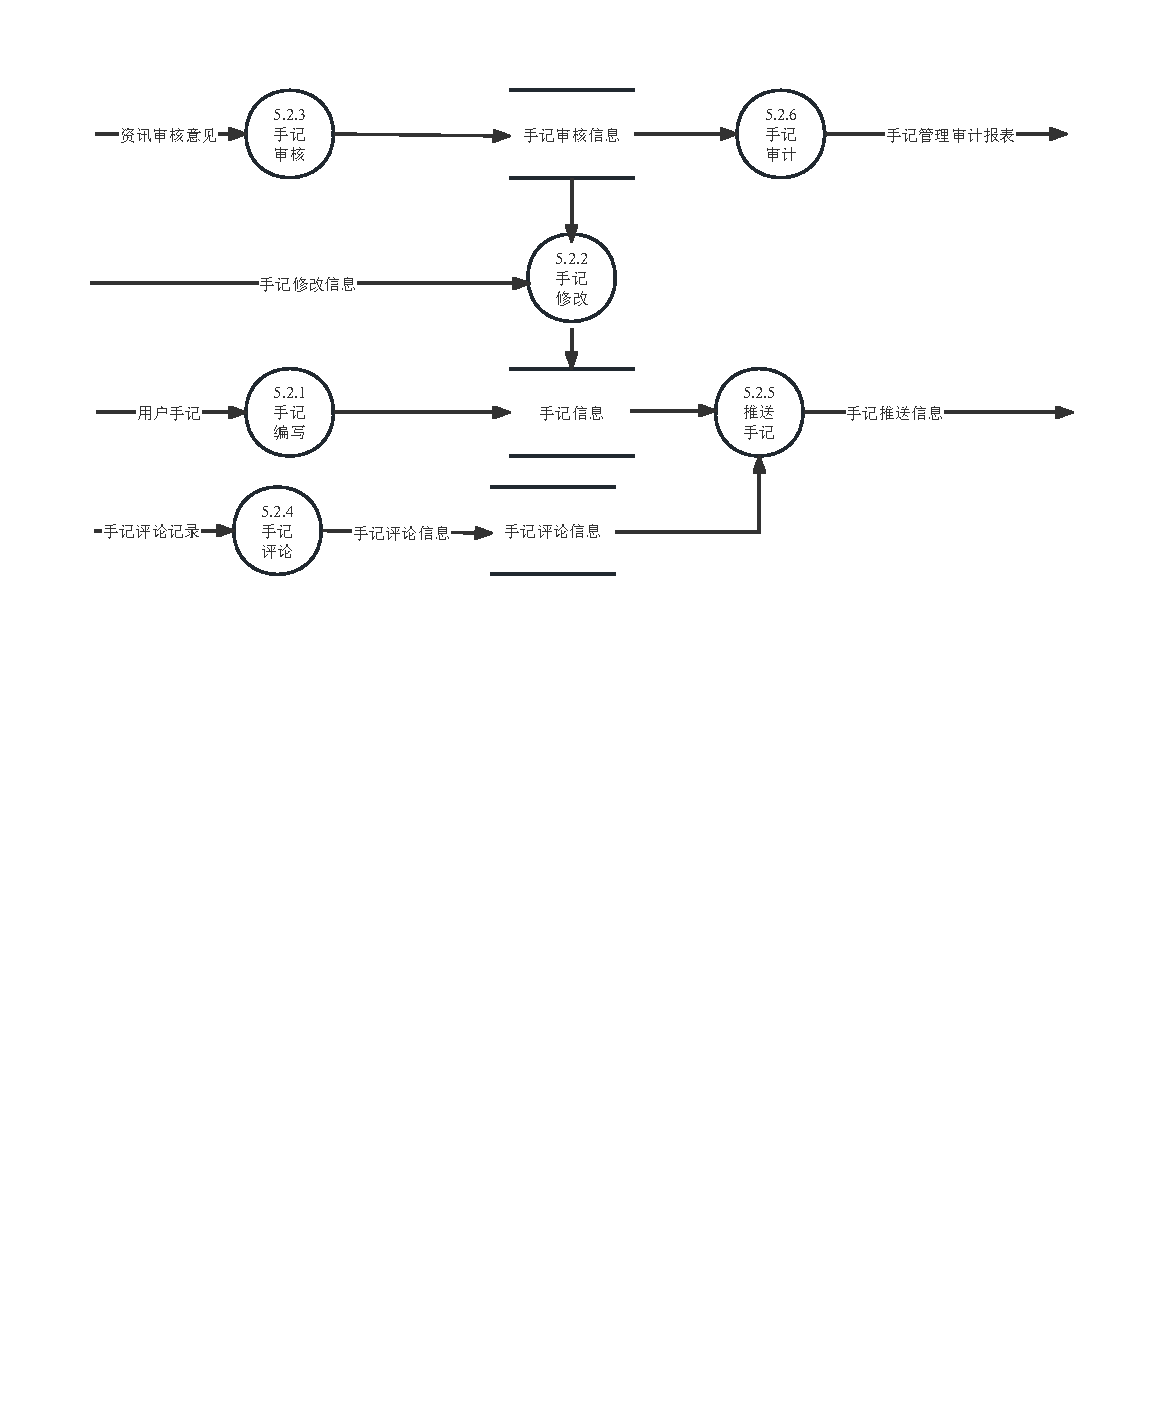
\includegraphics[width=0.95\textwidth]  {fig/论坛管理/F_2-2.pdf}} 
    \bicaption{交流论坛系统2层数据流图}{Data Flow Diagram for Level 2 of Communication Forum System}
    \end{figure}
    
(1)数据加工词条描述说明
\begin{table}[H]  
\caption{“手记编写”加工词条描述}  
\begin{center}  
    \begin{tabular}{l p{11cm}} 
        \hline
        \quad 名称:  &  手记编写 \\
        \hline
        \quad 编号:  & 5.2.1 \\
        \hline
        \quad 简述:  & 手记编写的功能 \\
        \hline
        \quad 输入:  & 手记编写信息 \\
        \hline
        \quad 输出:  & 手记信息 \\
        \hline
        \quad 逻辑:  & 保存用户资讯的内容信息。 \\
        \hline
    \end{tabular}
    \label{tab1}
\end{center}
\end{table}

\begin{algorithm}[H]
    \renewcommand{\thealgorithm}{}
    \caption{“手记编写”加工小说明} 
    \label{alg3} 
    \begin{algorithmic}[1]
        \STATE Create 手记ID
        \STATE Get 系统时间 As 发布时间
        \STATE Set 最后编辑时间 As 发布时间
        \STATE Write 手记信息 + 手记ID + 发布时间 +最后编辑时间 To 初始资讯信息
    \end{algorithmic} 
\end{algorithm}

\begin{table}[H]  
\caption{“手记修改”加工词条描述}  
\begin{center}  
    \begin{tabular}{l p{11cm}} 
        \hline
        \quad 名称:  &  手记修改 \\
        \hline
        \quad 编号:  & 5.2.2 \\
        \hline
        \quad 简述:  & 对手记进行修改的功能 \\
        \hline
        \quad 输入:  & 手记修改信息 \\
        \hline
        \quad 输出:  & 修改的手记信息 \\
        \hline
        \quad 逻辑:  & 完成用户修改手记的处理。 \\
        \hline
    \end{tabular}
    \label{tab1}
\end{center}
\end{table}

\begin{algorithm}[H] 
    \renewcommand{\thealgorithm}{}
    \caption{“手记修改”加工小说明} 
    \label{alg3} 
    \begin{algorithmic}[1]
        \STATE Get 手记ID From 手记修改信息
        \STATE Update Item In 手记信息 Match 手记ID With 资讯修改信息
    \end{algorithmic} 
\end{algorithm}

\begin{table}[H]  
\caption{“手记审核”加工词条描述}  
\begin{center}  
    \begin{tabular}{l p{11cm}} 
        \hline
        \quad 名称:  &  手记审核 \\
        \hline
        \quad 编号:  & 5.2.3 \\
        \hline
        \quad 简述:  & 系统管理员审核手记的功能 \\
        \hline
        \quad 输入:  & 手记审核意见 \\
        \hline
        \quad 输出:  & 手记审核信息 \\
        \hline
        \quad 逻辑:  & 系统管理员审核手记信息,并给出手记的修改要求。 \\
        \hline
    \end{tabular}
    \label{tab1}
\end{center}
\end{table}

\begin{algorithm}[H]
    \renewcommand{\thealgorithm}{}
    \caption{“手记审核”加工小说明} 
    \label{alg3} 
    \begin{algorithmic}[1]
        \STATE Get 系统时间 As 审核时间
        \STATE Write 手记审核意见 + 审核时间 To 手记审核信息
    \end{algorithmic} 
\end{algorithm}

\begin{table}[H]  
\caption{“手记评论”加工词条描述}  
\begin{center}  
    \begin{tabular}{l p{11cm}} 
        \hline
        \quad 名称:  &  手记评论 \\
        \hline
        \quad 编号:  & 5.2.4 \\
        \hline
        \quad 简述:  & 对手记进行评论的功能 \\
        \hline
        \quad 输入:  & 手记评论记录 \\
        \hline
        \quad 输出:  & 手记评论信息 \\
        \hline
        \quad 逻辑:  & 用户给出对手记的评论。 \\
        \hline
    \end{tabular}
    \label{tab1}
\end{center}
\end{table}

\begin{algorithm}[H]
    \renewcommand{\thealgorithm}{}
    \caption{“手记评论”加工小说明} 
    \label{alg3} 
    \begin{algorithmic}[1]
        \STATE Create 评论ID
        \STATE Get 系统时间 As 提交时间
        \STATE Write 手记评论记录+评论ID+提交时间+手记评论信息
    \end{algorithmic} 
\end{algorithm}

\begin{table}[H]  
\caption{“推送手记”加工词条描述}  
\begin{center}  
    \begin{tabular}{l p{11cm}} 
        \hline
        \quad 名称:  &  推送手记 \\
        \hline
        \quad 编号:  & 5.2.5 \\
        \hline
        \quad 简述:  & 对手记进推送的功能 \\
        \hline
        \quad 输入:  & 手记信息 \\
        \hline
        \quad 输出:  & 手记推送信息 \\
        \hline
        \quad 逻辑:  & 根据手记信息筛选出热度较高的手记推送信息。 \\
        \hline
    \end{tabular}
    \label{tab1}
\end{center}
\end{table}

\begin{algorithm}[H]
    \renewcommand{\thealgorithm}{}
    \caption{“手记推送”加工小说明} 
    \label{alg3} 
    \begin{algorithmic}[1]
        \STATE Analyze 手记信息
        \STATE Get 手记ID From 手记信息
        \STATE Select 对应手记评论 From 手记评论信息 Match 手记ID
        \STATE Write 手记信息 + 对应手记评论 To 手记推送信息
    \end{algorithmic} 
\end{algorithm}

\begin{table}[H]  
\caption{“手记审计”加工词条描述}  
\begin{center}  
    \begin{tabular}{l p{11cm}} 
        \hline
        \quad 名称:  & 手记审计 \\
        \hline
        \quad 编号:  & 5.2.6 \\
        \hline
        \quad 简述:  & 手记资讯的功能 \\
        \hline
        \quad 输入:  & 手记审核信息 \\
        \hline
        \quad 输出:  & 手记管理审计报表 \\
        \hline
        \quad 逻辑:  & 根据手记审核信息分析生成手记管理审计报表。 \\
        \hline
    \end{tabular}
    \label{tab1}
\end{center}
\end{table}

\begin{algorithm}[H]
    \renewcommand{\thealgorithm}{}
    \caption{“手记审计”加工小说明} 
    \label{alg3} 
    \begin{algorithmic}[1]
        \STATE Analyze 手记审核信息
        \STATE Generate 手记审核信息统计分析报表字段 Based On 手记审核信息
        \STATE Write 手记审核信息统计分析报表字段 To 手记审计报表
    \end{algorithmic} 
\end{algorithm}

(2)数据流词条描述说明
\begin{table}[H]  
\caption{``手记信息"数据流词条描述}  
\begin{center}  
    \begin{tabular}{l p{11cm}} 
        \hline
        \quad 名称:  &  手记信息 \\
        \hline
        \quad 简述:  & 志愿者手记的信息 \\
        \hline
        \quad 来源:  & 源点``志愿者" \\
        \hline
        \quad 去向:  & 加工``手记编写" \\
        \hline
        \quad 组成:  & 用户名+用户ID+手记标题+手记内容+发布时间+最后编辑时间 \\
        \hline
    \end{tabular}
    \label{tab1}
\end{center}
\end{table}

\begin{table}[H]  
\caption{``手记修改信息"数据流词条描述}  
\begin{center}  
    \begin{tabular}{l p{11cm}} 
        \hline
        \quad 名称:  &   手记修改信息 \\
        \hline
        \quad 简述:  & 修改后的手记信息 \\
        \hline
        \quad 来源:  & 源点``志愿者" \\
        \hline
        \quad 去想:  & 加工``手记修改" \\
        \hline
        \quad 组成:  & 用户名+用户ID+手记标题+编写时间+资讯内容+修改内容+修改说明+提交时间 \\
        \hline
    \end{tabular}
    \label{tab1}
\end{center}
\end{table}

\begin{table}[H]  
\caption{``手记审核意见"数据流词条描述}  
\begin{center}  
    \begin{tabular}{l p{11cm}} 
        \hline
        \quad 名称:  &   手记审核意见 \\
        \hline
        \quad 简述:  & 手记的审核意见 \\
        \hline
        \quad 来源:  & 源点``系统管理员" \\
        \hline
        \quad 去想:  & 加工``手记审核" \\
        \hline
        \quad 组成:  & 手记ID+修改要求+审核情况 \\
        \hline
    \end{tabular}
    \label{tab1}
\end{center}
\end{table}

\begin{table}[H]  
\caption{``手记评论记录"数据流词条描述}  
\begin{center}  
    \begin{tabular}{l p{11cm}} 
        \hline
        \quad 名称:  &   手记评论记录 \\
        \hline
        \quad 简述:  & 手记评论的记录信息 \\
        \hline
        \quad 来源:  & 源点``志愿者" \\
        \hline
        \quad 去想:  & 加工``手记评论" \\
        \hline
        \quad 组成:  & 手记ID+评论内容+用户ID+用户名 \\
        \hline
    \end{tabular}
    \label{tab1}
\end{center}
\end{table}

\begin{table}[H]  
\caption{``推送信息"数据流词条描述}  
\begin{center}  
    \begin{tabular}{l p{11cm}} 
        \hline
        \quad 名称:  &   推送信息 \\
        \hline
        \quad 简述:  & 推送的手记信息 \\
        \hline
        \quad 来源:  & 加工``手记推送" \\
        \hline
        \quad 去想:  & 源点``志愿者" \\
        \hline
        \quad 组成:  & 手记标题+手机内容+评论内容+发布时间 \\
        \hline
    \end{tabular}
    \label{tab1}
\end{center}
\end{table}

\begin{table}[H]  
\caption{``手记管理审计报表"数据流词条描述}  
\begin{center}  
    \begin{tabular}{l p{11cm}} 
        \hline
        \quad 名称:  &  手记管理审计报表 \\
        \hline
        \quad 简述:  & 手记管理模块的审计报表 \\
        \hline
        \quad 来源:  & 加工``手记审计" \\
        \hline
        \quad 去向:  & 源点``政府相关部门" \\
        \hline
        \quad 组成:  & 手记审核信息统计分析报表字段\\
        \hline
    \end{tabular}
    \label{tab1}
\end{center}
\end{table}


(3)文件词条描述
\begin{table}[H]  
\caption{“手记信息”文件词条描述}  
\begin{center}  
    \begin{tabular}{l p{10cm}} 
        \hline
        \quad 名称:  &   手记信息 \\
        \hline
        \quad 简述:  & 存储手记内容\\
        \hline
        \quad 组成:  & 手记ID+用户ID+用户名+手记标题+手记内容+修改内容+发布时间+最后编辑时间 \\
        \hline
        \quad 存储方式:  & 以手记ID为关键字。 \\
        \hline
    \end{tabular}
    \label{tab1}
\end{center}
\end{table}

\begin{table}[H]  
\caption{“手记评论信息”文件词条描述}  
\begin{center}  
    \begin{tabular}{l p{10cm}} 
        \hline
        \quad 名称:  &  手记评论信息 \\
        \hline
        \quad 简述:  & 存储用户对手记的评论 \\
        \hline
        \quad 组成:  & 评论ID+资讯ID+用户ID+评论内容+提交时间 \\
        \hline
        \quad 存储方式:  & 以评论ID为关键字。 \\
        \hline
    \end{tabular}
    \label{tab1}
\end{center}
\end{table}

\begin{table}[H]  
\caption{“手记审核信息”文件词条描述}  
\begin{center}  
    \begin{tabular}{l p{10cm}} 
        \hline
        \quad 名称:  &  手记审核信息 \\
        \hline
        \quad 简述:  & 存储管理员对手记的审核意见 \\
        \hline
        \quad 组成:  & 手记ID + 修改要求 + 审核情况 + 审核时间 \\
        \hline
        \quad 存储方式:  & 以手记ID为关键字。 \\
        \hline
    \end{tabular}
    \label{tab1}
\end{center}
\end{table}


\paragraph{交流管理}~{}
\\
\begin{figure}[H]
    \center{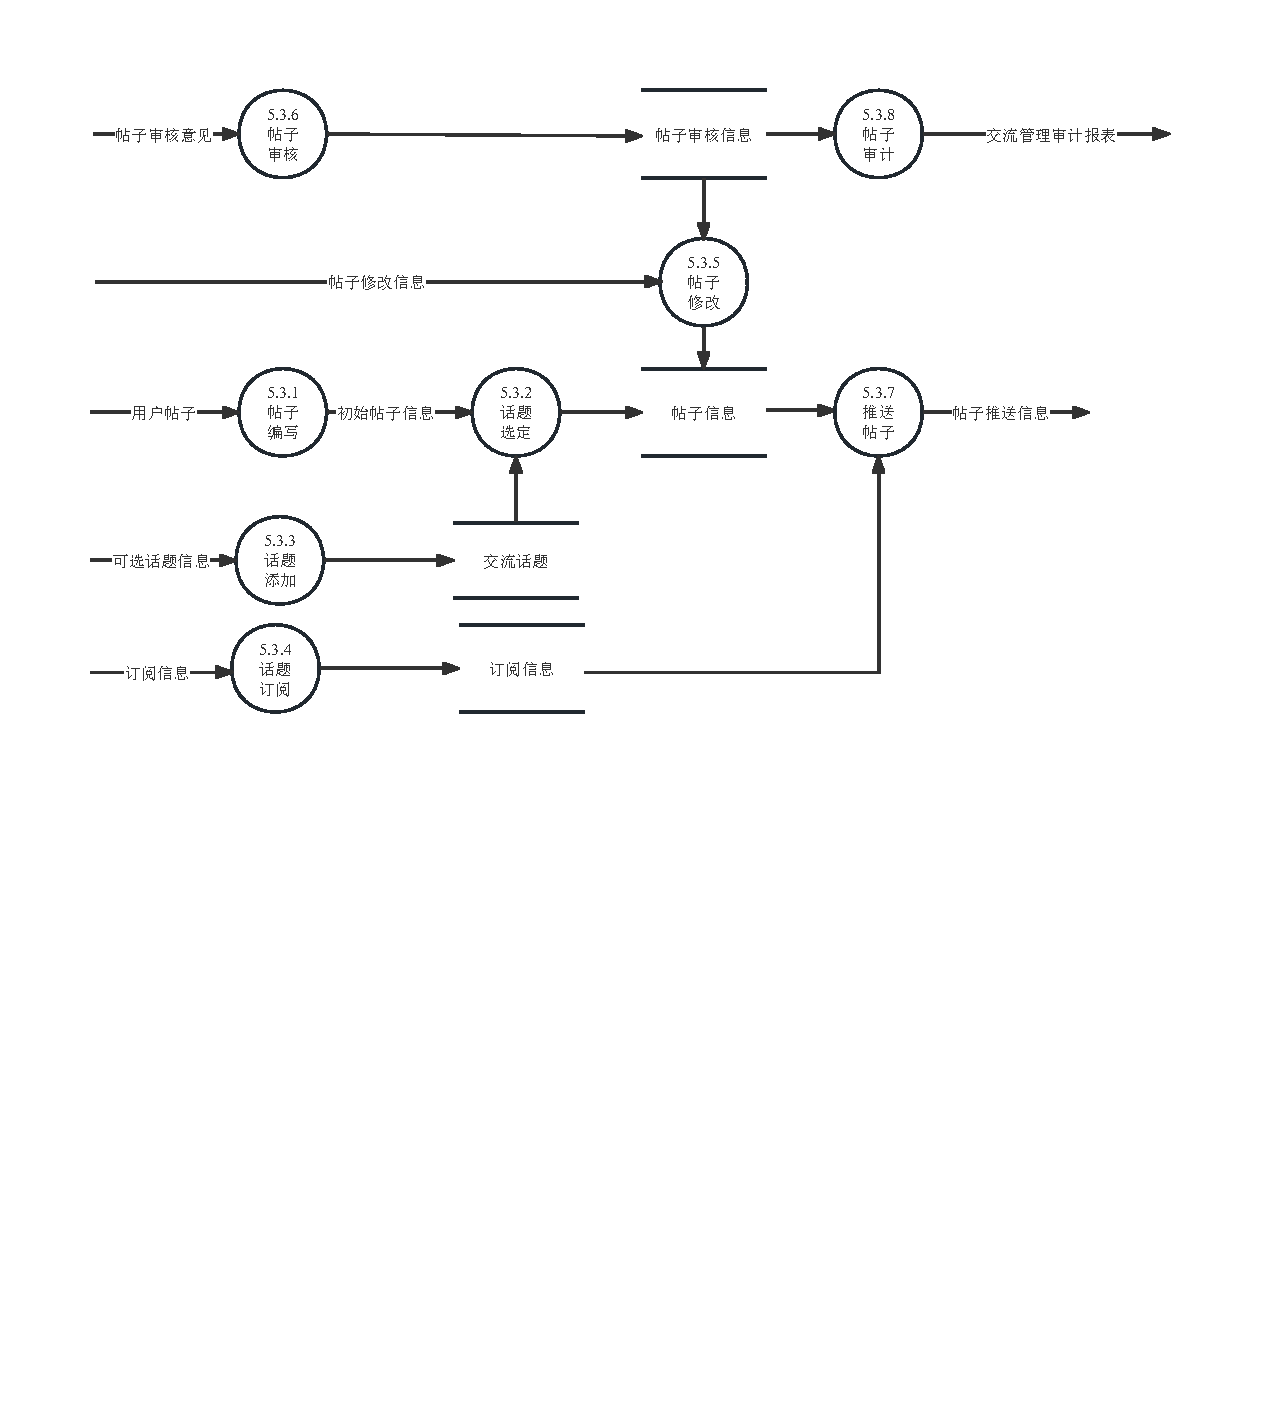
\includegraphics[width=0.95\textwidth]  {fig/论坛管理/F_2-3.pdf}} 
    \bicaption{交流论坛系统2层数据流图}{Data Flow Diagram for Level 2 of Communication Forum System}
    \end{figure}
    
(1)数据加工词条描述说明
\begin{table}[H]  
\caption{“帖子编写”加工词条描述}  
\begin{center}  
    \begin{tabular}{l p{11cm}} 
        \hline
        \quad 名称:  &  帖子编写 \\
        \hline
        \quad 编号:  & 5.3.1 \\
        \hline
        \quad 简述:  & 帖子编写的功能 \\
        \hline
        \quad 输入:  & 帖子编写信息 \\
        \hline
        \quad 输出:  & 帖子信息 \\
        \hline
        \quad 逻辑:  & 保存用户帖子的内容信息。 \\
        \hline
    \end{tabular}
    \label{tab1}
\end{center}
\end{table}

\begin{algorithm}[H]
    \renewcommand{\thealgorithm}{}
    \caption{“帖子编写”加工小说明} 
    \label{alg3} 
    \begin{algorithmic}[1]
        \STATE Create 帖子ID
        \STATE Get 系统时间 As 发布时间
        \STATE Set 最后编辑时间 As 发布时间
        \STATE Write 用户帖子 + 帖子ID + 发布时间 +最后编辑时间 To 初始帖子信息
    \end{algorithmic} 
\end{algorithm}

\begin{table}[H]  
\caption{“话题选定”加工词条描述}  
\begin{center}  
    \begin{tabular}{l p{11cm}} 
        \hline
        \quad 名称:  &  话题选定 \\
        \hline
        \quad 编号:  & 5.3.2 \\
        \hline
        \quad 简述:  & 用户选择话题的功能 \\
        \hline
        \quad 输入:  & 可选话题信息、帖子话题选择信息 \\
        \hline
        \quad 输出:  & 话题选择信息 \\
        \hline
        \quad 逻辑:  & 帖子话题信息提供可选话题信息给用户,用户根据可选话题信息给出话题选择信息。 \\
        \hline
    \end{tabular}
    \label{tab1}
\end{center}
\end{table}

\begin{algorithm}[H]
    \renewcommand{\thealgorithm}{}
    \caption{“话题选定”加工小说明} 
    \label{alg3} 
    \begin{algorithmic}[1]
        \STATE Generate 话题ID + 话题名 Based On 初始帖子信息
        \STATE Write 初始话题信息 + 话题ID + 话题名 To 帖子信息
    \end{algorithmic} 
\end{algorithm}

\begin{table}[H]  
\caption{“话题订阅”加工词条描述}  
\begin{center}  
    \begin{tabular}{l p{11cm}} 
        \hline
        \quad 名称:  &  话题订阅 \\
        \hline
        \quad 编号:  & 5.3.3 \\
        \hline
        \quad 简述:  & 对话题进行订阅的功能 \\
        \hline
        \quad 输入:  & 话题订阅记录 \\
        \hline
        \quad 输出:  & 话题订阅信息 \\
        \hline
        \quad 逻辑:  & 用户对话题进行订阅。 \\
        \hline
    \end{tabular}
    \label{tab1}
\end{center}
\end{table}

\begin{algorithm}[H]
    \renewcommand{\thealgorithm}{}
    \caption{“话题订阅”加工小说明} 
    \label{alg3} 
    \begin{algorithmic}[1]
        \STATE Insert 用户ID + 话题ID Into 订阅信息
    \end{algorithmic} 
\end{algorithm}


\begin{table}[H]  
\caption{“帖子修改”加工词条描述}  
\begin{center}  
    \begin{tabular}{l p{11cm}} 
        \hline
        \quad 名称:  &  帖子修改 \\
        \hline
        \quad 编号:  & 5.3.4 \\
        \hline
        \quad 简述:  & 对帖子进行修改的功能 \\
        \hline
        \quad 输入:  & 帖子修改信息 \\
        \hline
        \quad 输出:  & 修改的帖子信息 \\
        \hline
        \quad 逻辑:  & 完成用户修改帖子的处理。 \\
        \hline
    \end{tabular}
    \label{tab1}
\end{center}
\end{table}

\begin{algorithm}[H] 
    \renewcommand{\thealgorithm}{}
    \caption{“帖子修改”加工小说明} 
    \label{alg3} 
    \begin{algorithmic}[1]
        \STATE Get 帖子ID From 帖子修改信息
        \STATE Update Item In 帖子信息 Match 帖子ID With 帖子修改信息
    \end{algorithmic} 
\end{algorithm}

\begin{table}[H]  
\caption{“帖子审核”加工词条描述}  
\begin{center}  
    \begin{tabular}{l p{11cm}} 
        \hline
        \quad 名称:  &  帖子审核 \\
        \hline
        \quad 编号:  & 5.3.5 \\
        \hline
        \quad 简述:  & 系统管理员审核帖子的功能 \\
        \hline
        \quad 输入:  & 帖子审核意见 \\
        \hline
        \quad 输出:  & 帖子审核信息 \\
        \hline
        \quad 逻辑:  & 系统管理员审核帖子信息,并给出帖子的修改要求。 \\
        \hline
    \end{tabular}
    \label{tab1}
\end{center}
\end{table}

\begin{algorithm}[H]
    \renewcommand{\thealgorithm}{}
    \caption{“帖子审核”加工小说明} 
    \label{alg3} 
    \begin{algorithmic}[1]
        \STATE Get 系统时间 As 审核时间
        \STATE Write 帖子审核意见 + 审核时间 To 帖子审核信息
    \end{algorithmic} 
\end{algorithm}

\begin{table}[H]  
\caption{“推送帖子”加工词条描述}  
\begin{center}  
    \begin{tabular}{l p{11cm}} 
        \hline
        \quad 名称:  &  帖子审核 \\
        \hline
        \quad 编号:  & 5.3.6 \\
        \hline
        \quad 简述:  & 推送帖子的功能 \\
        \hline
        \quad 输入:  & 帖子信息 \\
        \hline
        \quad 输出:  & 帖子推送 \\
        \hline
        \quad 逻辑:  & 根据帖子信息筛选出热度较高的手记推送信息\\
        \hline
    \end{tabular}
    \label{tab1}
\end{center}
\end{table}

\begin{algorithm}[H]
    \renewcommand{\thealgorithm}{}
    \caption{“帖子推送”加工小说明} 
    \label{alg3} 
    \begin{algorithmic}[1]
        \STATE Analyze 帖子信息
        \FOR{ 用户ID + 话题ID in 订阅信息}
        \STATE Select 对应帖子信息 From 帖子信息 Match 话题ID
        \STATE Add 对应手记评论+用户ID To 帖子推送信息
        \ENDFOR
    \end{algorithmic} 
\end{algorithm}

\begin{table}[H]  
\caption{“帖子审计”加工词条描述}  
\begin{center}  
    \begin{tabular}{l p{11cm}} 
        \hline
        \quad 名称:  & 帖子审计 \\
        \hline
        \quad 编号:  & 5.3.7 \\
        \hline
        \quad 简述:  & 审计帖子的功能 \\
        \hline
        \quad 输入:  & 帖子审核信息 \\
        \hline
        \quad 输出:  & 交流管理审计报表 \\
        \hline
        \quad 逻辑:  & 根据帖子审核信息分析生成交流管理审计报表。 \\
        \hline
    \end{tabular}
    \label{tab1}
\end{center}
\end{table}

\begin{algorithm}[H]
    \renewcommand{\thealgorithm}{}
    \caption{“帖子审计”加工小说明} 
    \label{alg3} 
    \begin{algorithmic}[1]
        \STATE Analyze 帖子审核信息
        \STATE Generate 帖子审核信息统计分析报表字段 Based On 帖子审核信息
        \STATE Write 帖子审核信息统计分析报表字段 To 帖子审计报表
    \end{algorithmic} 
\end{algorithm}

(2)数据流词条描述说明
\begin{table}[H]  
\caption{``用户帖子"数据流词条描述}  
\begin{center}  
    \begin{tabular}{l p{11cm}} 
        \hline
        \quad 名称:  &  用户帖子 \\
        \hline
        \quad 简述:  & 志用户帖子的信息 \\
        \hline
        \quad 来源:  & 源点``志愿者" \\
        \hline
        \quad 去向:  & 加工``帖子编写" \\
        \hline
        \quad 组成:  & 用户名+用户ID+帖子内容+发布时间+最后编辑时间 \\
        \hline
    \end{tabular}
    \label{tab1}
\end{center}
\end{table}

\begin{table}[H]  
\caption{``初始帖子信息"数据流词条描述}  
\begin{center}  
    \begin{tabular}{l p{11cm}} 
        \hline
        \quad 名称:  &   初始帖子信息 \\
        \hline
        \quad 简述:  & 未选定话题的帖子信息 \\
        \hline
        \quad 来源:  & 加工``帖子编写" \\
        \hline
        \quad 去向:  & 加工``话题选定" \\
        \hline
        \quad 组成:  & 用户名+用户ID+话题ID+话题名+帖子内容+发布时间+最后编辑时间 \\
        \hline
    \end{tabular}
    \label{tab1}
\end{center}
\end{table}

\begin{table}[H]  
\caption{``订阅信息"数据流词条描述}  
\begin{center}  
    \begin{tabular}{l p{11cm}} 
        \hline
        \quad 名称:  & 订阅信息 \\
        \hline
        \quad 简述:  & 帖子的审核意见 \\
        \hline
        \quad 来源:  & 源点``用户" \\
        \hline
        \quad 去向:  & 加工``话题订阅" \\
        \hline
        \quad 组成:  & 用户ID + 话题ID \\
        \hline
    \end{tabular}
    \label{tab1}
\end{center}
\end{table}

\begin{table}[H]  
\caption{``可选话题信息"数据流词条描述}  
\begin{center}  
    \begin{tabular}{l p{11cm}} 
        \hline
        \quad 名称:  &  可选话题信息 \\
        \hline
        \quad 简述:  & 可选的话题信息 \\
        \hline
        \quad 来源:  & 源点``系统管理员" \\
        \hline
        \quad 去向:  & 加工``话题设置" \\
        \hline
        \quad 组成:  & 话题ID+话题名 \\
        \hline
    \end{tabular}
    \label{tab1}
\end{center}
\end{table}

\begin{table}[H]  
\caption{``帖子推送信息"数据流词条描述}  
\begin{center}  
    \begin{tabular}{l p{11cm}} 
        \hline
        \quad 名称:  &  帖子推送信息信息 \\
        \hline
        \quad 简述:  & 推送的帖子信息 \\
        \hline
        \quad 来源:  & 加工``推送帖子" \\
        \hline
        \quad 去向:  & 源点``志愿者" \\
        \hline
        \quad 组成:  & 话题名+用户名+帖子内容+发布时间+推送到的用户ID \\
        \hline
    \end{tabular}
    \label{tab1}
\end{center}
\end{table}


\begin{table}[H]  
\caption{``交流管理审计报表"数据流词条描述}  
\begin{center}  
    \begin{tabular}{l p{11cm}} 
        \hline
        \quad 名称:  & 交流管理审计报表 \\
        \hline
        \quad 简述:  & 交流管理模块的审计报表 \\
        \hline
        \quad 来源:  & 加工``交流审计" \\
        \hline
        \quad 去向:  & 源点``政府相关部门" \\
        \hline
        \quad 组成:  & 帖子审核信息统计分析报表字段 \\
        \hline
    \end{tabular}
    \label{tab1}
\end{center}
\end{table}



(3)文件词条描述
\begin{table}[H]  
\caption{“帖子信息”文件词条描述}  
\begin{center}  
    \begin{tabular}{l p{10cm}} 
        \hline
        \quad 名称:  & 资讯信息 \\
        \hline
        \quad 简述:  & 存储资讯内容\\
        \hline
        \quad 组成:  & 帖子ID+用户ID+用户名+话题ID+话题名+帖子内容+修改内容+发布时间+最后编辑时间 \\
        \hline
        \quad 存储方式:  & 以帖子ID为关键字。 \\
        \hline
    \end{tabular}
    \label{tab1}
\end{center}
\end{table}

\begin{table}[H]  
\caption{“交流话题”文件词条描述}  
\begin{center}  
    \begin{tabular}{l p{10cm}} 
        \hline
        \quad 名称:  &  资讯分类信息 \\
        \hline
        \quad 简述:  & 系统中资讯分类类别的相关信息 \\
        \hline
        \quad 组成:  & 话题ID+话题名 \\
        \hline
        \quad 存储方式:  & 以话题ID为关键字。 \\
        \hline
    \end{tabular}
    \label{tab1}
\end{center}
\end{table}

\begin{table}[H]  
\caption{“订阅信息”文件词条描述}  
\begin{center}  
    \begin{tabular}{l p{10cm}} 
        \hline
        \quad 名称:  &   订阅信息 \\
        \hline
        \quad 简述:  & 存储用户订阅话题的信息 \\
        \hline
        \quad 组成:  & 用户ID+话题ID \\
        \hline
        \quad 存储方式:  & 以用户ID、话题ID为关键字。 \\
        \hline
    \end{tabular}
    \label{tab1}
\end{center}
\end{table}

\begin{table}[H]  
\caption{“帖子审核信息”文件词条描述}  
\begin{center}  
    \begin{tabular}{l p{10cm}} 
        \hline
        \quad 名称:  &  帖子审核信息 \\
        \hline
        \quad 简述:  & 存储管理员对帖子的审核意见 \\
        \hline
        \quad 组成:  & 帖子ID + 修改要求 + 审核情况 + 审核时间 \\
        \hline
        \quad 存储方式:  & 以帖子ID为关键字。 \\
        \hline
    \end{tabular}
    \label{tab1}
\end{center}
\end{table}

\subsubsection{志愿交友系统}
以下是志愿交友系统的 1 层数据流图、加工子图以及对应的数据字典和文件。
\begin{figure}[H]
    \center{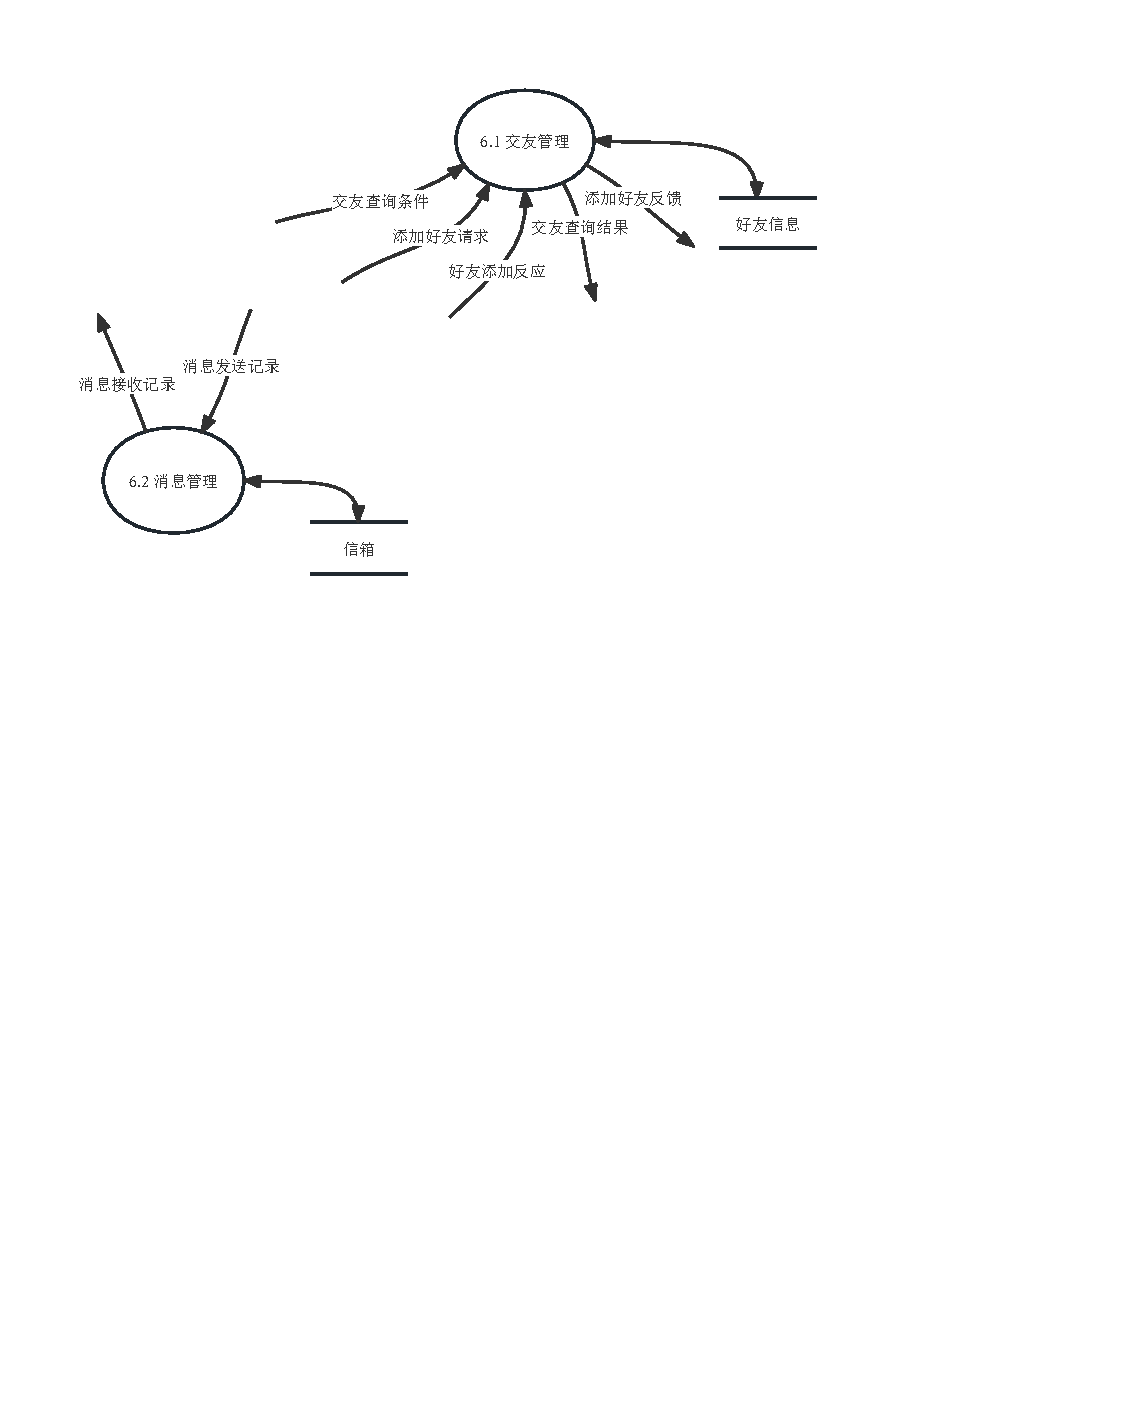
\includegraphics[width=0.95\textwidth]  {fig/社交管理/S_1.pdf}} 
    \bicaption{志愿交友系统1层数据流图}{Data Flow Diagram for Level 1 of Volunteer Social System}
    \end{figure}
    
\paragraph{交友管理}~{}
\\
\begin{figure}[H]
    \center{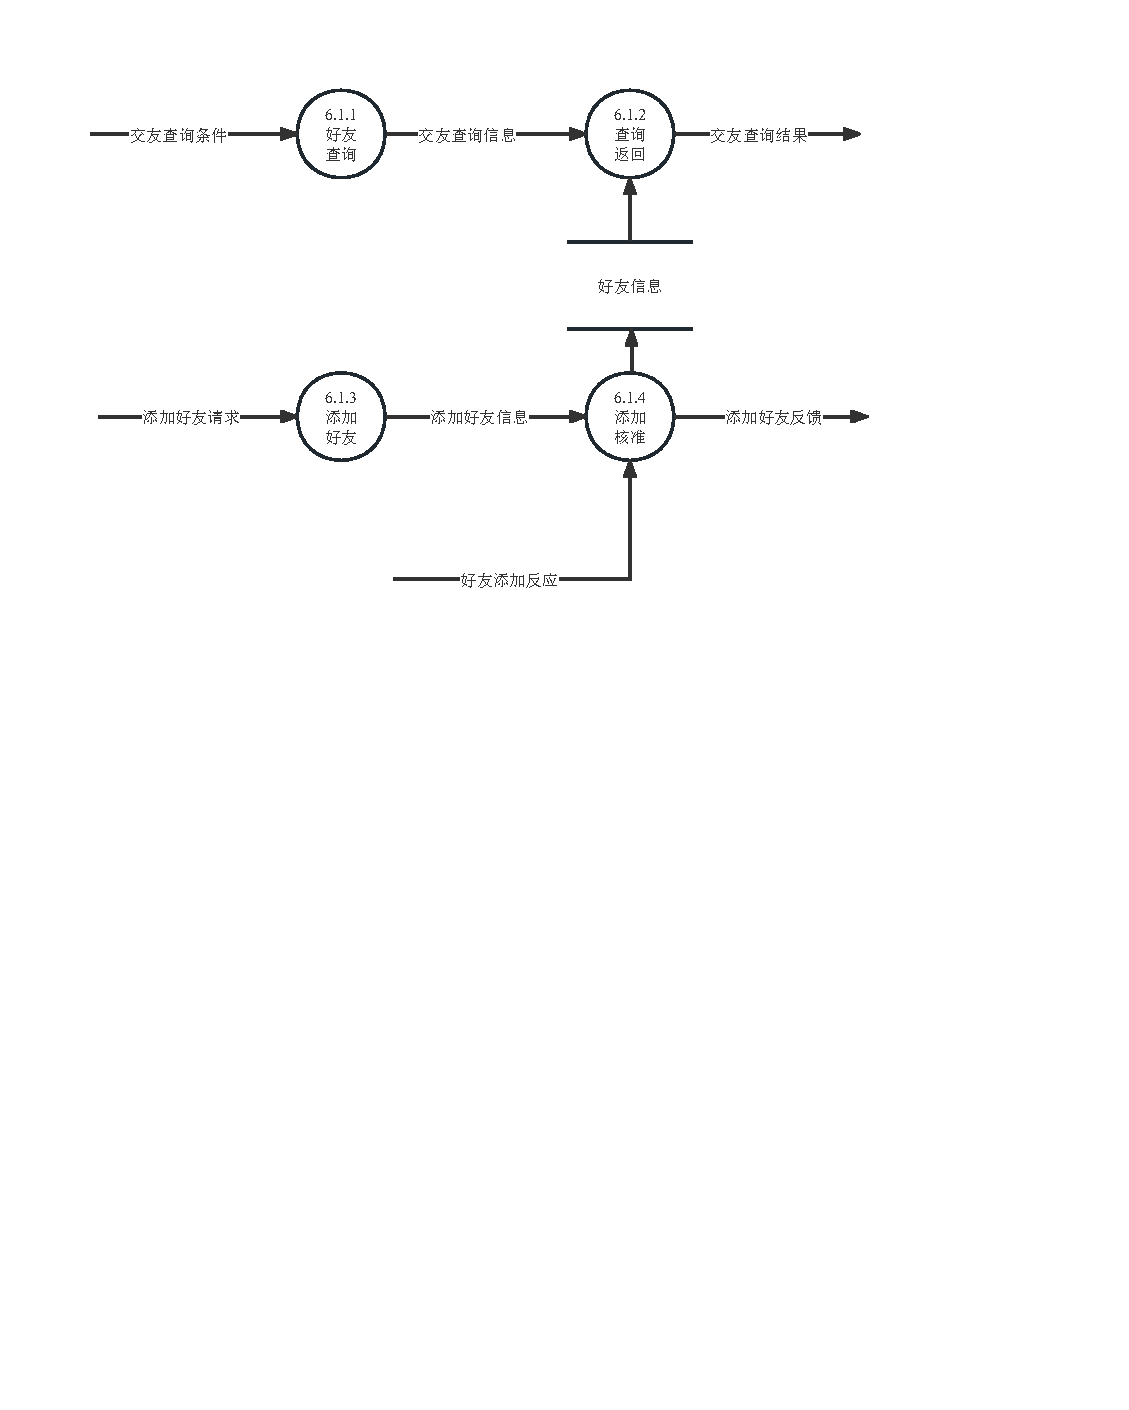
\includegraphics[width=0.95\textwidth]  {fig/社交管理/S_2-1.pdf}} 
    \bicaption{志愿交友系统2层数据流图}{Data Flow Diagram for Level 2 of Volunteer Social System}
    \end{figure}
    
(1)数据加工词条描述说明
\begin{table}[H]  
\caption{“添加好友”加工词条描述}  
\begin{center}  
    \begin{tabular}{l p{11cm}} 
        \hline
        \quad 名称:  &  添加好友 \\
        \hline
        \quad 编号:  & 6.1.1 \\
        \hline
        \quad 简述:  & 申请添加好友的功能 \\
        \hline
        \quad 输入:  & 添加好友请求\\
        \hline
        \quad 输出:  & 添加好友信息 \\
        \hline
        \quad 逻辑:  & 根据添加好友的请求,生成添加好友信息。 \\
        \hline
    \end{tabular}
    \label{tab1}
\end{center}
\end{table}

\begin{algorithm}[H]
    \renewcommand{\thealgorithm}{}
    \caption{“添加好友”加工小说明} 
    \label{alg3} 
    \begin{algorithmic}[1]
        \STATE Get 系统时间 As 添加时间
        \STATE Write 添加好友请求 + 添加时间 To 添加好友信息
    \end{algorithmic} 
\end{algorithm}

\begin{table}[H]  
\caption{“添加核准”加工词条描述}  
\begin{center}  
    \begin{tabular}{l p{11cm}} 
        \hline
        \quad 名称:  &   添加核准 \\
        \hline
        \quad 编号:  & 6.1.2 \\
        \hline
        \quad 简述:  & 添加好友行为的功能 \\
        \hline
        \quad 输入:  & 好友添加反应\\
        \hline
        \quad 输出:  & 好友添加反馈、好友信息 \\
        \hline
        \quad 逻辑:  & 根据添加好友信息,生成添加反馈,同意则将好友加入好友信息。 \\
        \hline
    \end{tabular}
    \label{tab1}
\end{center}
\end{table}

\begin{algorithm}[H]
    \renewcommand{\thealgorithm}{}
    \caption{“添加核准”加工小说明} 
    \label{alg3} 
    \begin{algorithmic}[1]
        \IF{好友添加反应通过} 
        \STATE Write 用户1的ID + 用户2的ID to 好友信息 
        \STATE Write {理由} + 反应时间  To 好友添加反馈
        \ELSE
        \STATE Write {理由} + 反应时间  To 好友添加反馈
        \ENDIF 
    \end{algorithmic} 
\end{algorithm}

\begin{table}[H]  
\caption{“好友查询”加工词条描述}  
\begin{center}  
    \begin{tabular}{l p{11cm}} 
        \hline
        \quad 名称:  &   好友查询 \\
        \hline
        \quad 编号:  & 6.1.3 \\
        \hline
        \quad 简述:  & 查询用户的好友 \\
        \hline
        \quad 输入:  & 查询条件 \\
        \hline
        \quad 输出:  & 查询信息\\
        \hline
        \quad 逻辑:  & 根据查询条件产生完整的查询信息。 \\
        \hline
    \end{tabular}
    \label{tab1}
\end{center}
\end{table}

\begin{algorithm}[H] 
    \renewcommand{\thealgorithm}{}
    \caption{“好友查询”加工小说明} 
    \label{alg3} 
    \begin{algorithmic}[1]
        \STATE Get 系统时间 As 查询时间
        \STATE Write 交友查询条件 + 查询时间 To 交友查询信息 
    \end{algorithmic} 
\end{algorithm}


\begin{table}[H]  
\caption{“查询返回”加工词条描述}  
\begin{center}  
    \begin{tabular}{l p{11cm}} 
        \hline
        \quad 名称:  &  查询返回 \\
        \hline
        \quad 编号:  & 6.1.4 \\
        \hline
        \quad 简述:  & 返回查询结果的功能 \\
        \hline
        \quad 输入:  & 查询信息、好友信息 \\
        \hline
        \quad 输出:  & 查询结果\\
        \hline
        \quad 逻辑:  & 根据查询信息,筛选符合的好友信息组成查询结果。 \\
        \hline
    \end{tabular}
    \label{tab1}
\end{center}
\end{table}

\begin{algorithm}[H] 
    \renewcommand{\thealgorithm}{}
    \caption{“查询返回”加工小说明} 
    \label{alg3} 
    \begin{algorithmic}[1]
        \STATE Select Items In 好友信息 Match 交友查询信息
        \STATE Write Selected Items As 交友查询结果
    \end{algorithmic} 
\end{algorithm}

(2)数据流词条描述说明
\begin{table}[H]  
\caption{``添加好友请求"数据流词条描述}  
\begin{center}  
    \begin{tabular}{l p{11cm}} 
        \hline
        \quad 名称:  &  添加好友请求 \\
        \hline
        \quad 简述:  & 添加好友请求的信息 \\
        \hline
        \quad 来源:  & 源点``志愿者" \\
        \hline
        \quad 去向:  & 加工``添加好友" \\
        \hline
        \quad 组成:  & 用户ID +用户名+添加留言 \\
        \hline
    \end{tabular}
    \label{tab1}
\end{center}
\end{table}

\begin{table}[H]  
\caption{``添加好友信息"数据流词条描述}  
\begin{center}  
    \begin{tabular}{l p{11cm}} 
        \hline
        \quad 名称:  &   添加好友信息 \\
        \hline
        \quad 简述:  & 申请添加好友的信息 \\
        \hline
        \quad 来源:  & 加工``添加好友" \\
        \hline
        \quad 去向:  & 加工``添加核准" \\
        \hline
        \quad 组成:  & 用户ID +用户名+添加留言+添加时间 \\
        \hline
    \end{tabular}
    \label{tab1}
\end{center}
\end{table}

\begin{table}[H]  
\caption{``好友添加反应"数据流词条描述}  
\begin{center}  
    \begin{tabular}{l p{11cm}} 
        \hline
        \quad 名称:  &   添加好友反应 \\
        \hline
        \quad 简述:  & 对于添加好友是否同意的反应 \\
        \hline
        \quad 来源:  & 源点``志愿者" \\
        \hline
        \quad 去向:  & 加工``添加反馈" \\
        \hline
        \quad 组成:  & 用户ID +用户名+操作+{理由}+反应时间 \\
        \hline
    \end{tabular}
    \label{tab1}
\end{center}
\end{table}

\begin{table}[H]  
\caption{``好友添加反馈"数据流词条描述}  
\begin{center}  
    \begin{tabular}{l p{11cm}} 
        \hline
        \quad 名称:  &   添加好友反馈 \\
        \hline
        \quad 简述:  & 对于对方反应的反馈 \\
        \hline
        \quad 来源:  & 加工``添加反馈" \\
        \hline
        \quad 去向:  & 源点``志愿者" \\
        \hline
        \quad 组成:  & 用户名+理由+反应时间 \\
        \hline
    \end{tabular}
    \label{tab1}
\end{center}
\end{table}

\begin{table}[H]  
\caption{``交友查询条件"数据流词条描述}  
\begin{center}  
    \begin{tabular}{l p{11cm}} 
        \hline
        \quad 名称:  &  交友查询条件 \\
        \hline
        \quad 简述:  & 用户查询好友的条件 \\
        \hline
        \quad 来源:  & 源点``志愿者"\\
        \hline
        \quad 去向:  & 加工``好友查询" \\
        \hline
        \quad 组成:  & 查询关键字\\
        \hline
    \end{tabular}
    \label{tab1}
\end{center}
\end{table}

\begin{table}[H]  
\caption{``交友查询信息"数据流词条描述}  
\begin{center}  
    \begin{tabular}{l p{11cm}} 
        \hline
        \quad 名称:  &   交友查询信息 \\
        \hline
        \quad 简述:  & 用户对好友查询的完整信息 \\
        \hline
        \quad 来源:  & 加工``好友查询"\\
        \hline
        \quad 去向:  & 加工``查询返回" \\
        \hline
        \quad 组成:  & 用户ID +查询关键字\\
        \hline
    \end{tabular}
    \label{tab1}
\end{center}
\end{table}

\begin{table}[H]  
\caption{``交友查询结果"数据流词条描述}  
\begin{center}  
    \begin{tabular}{l p{11cm}} 
        \hline
        \quad 名称:  &   交友查询结果 \\
        \hline
        \quad 简述:  & 符合条件的好友信息 \\
        \hline
        \quad 来源:  & 加工``查询返回"\\
        \hline
        \quad 去向:  & 源点``志愿者" \\
        \hline
        \quad 组成:  & 用户名\\
        \hline
    \end{tabular}
    \label{tab1}
\end{center}
\end{table}


(3)文件词条描述
\begin{table}[H]  
\caption{“好友信息”文件词条描述}  
\begin{center}  
    \begin{tabular}{l p{10cm}} 
        \hline
        \quad 名称:  &   好友信息 \\
        \hline
        \quad 简述:  & 存储用户好友信息内容\\
        \hline
        \quad 组成:  & 用户1ID+用户2ID \\
        \hline
        \quad 存储方式:  & 以用户1的ID、用户2的ID为关键字。 \\
        \hline
    \end{tabular}
    \label{tab1}
\end{center}
\end{table}



\paragraph{消息管理}~{}
\\
\begin{figure}[H]
    \center{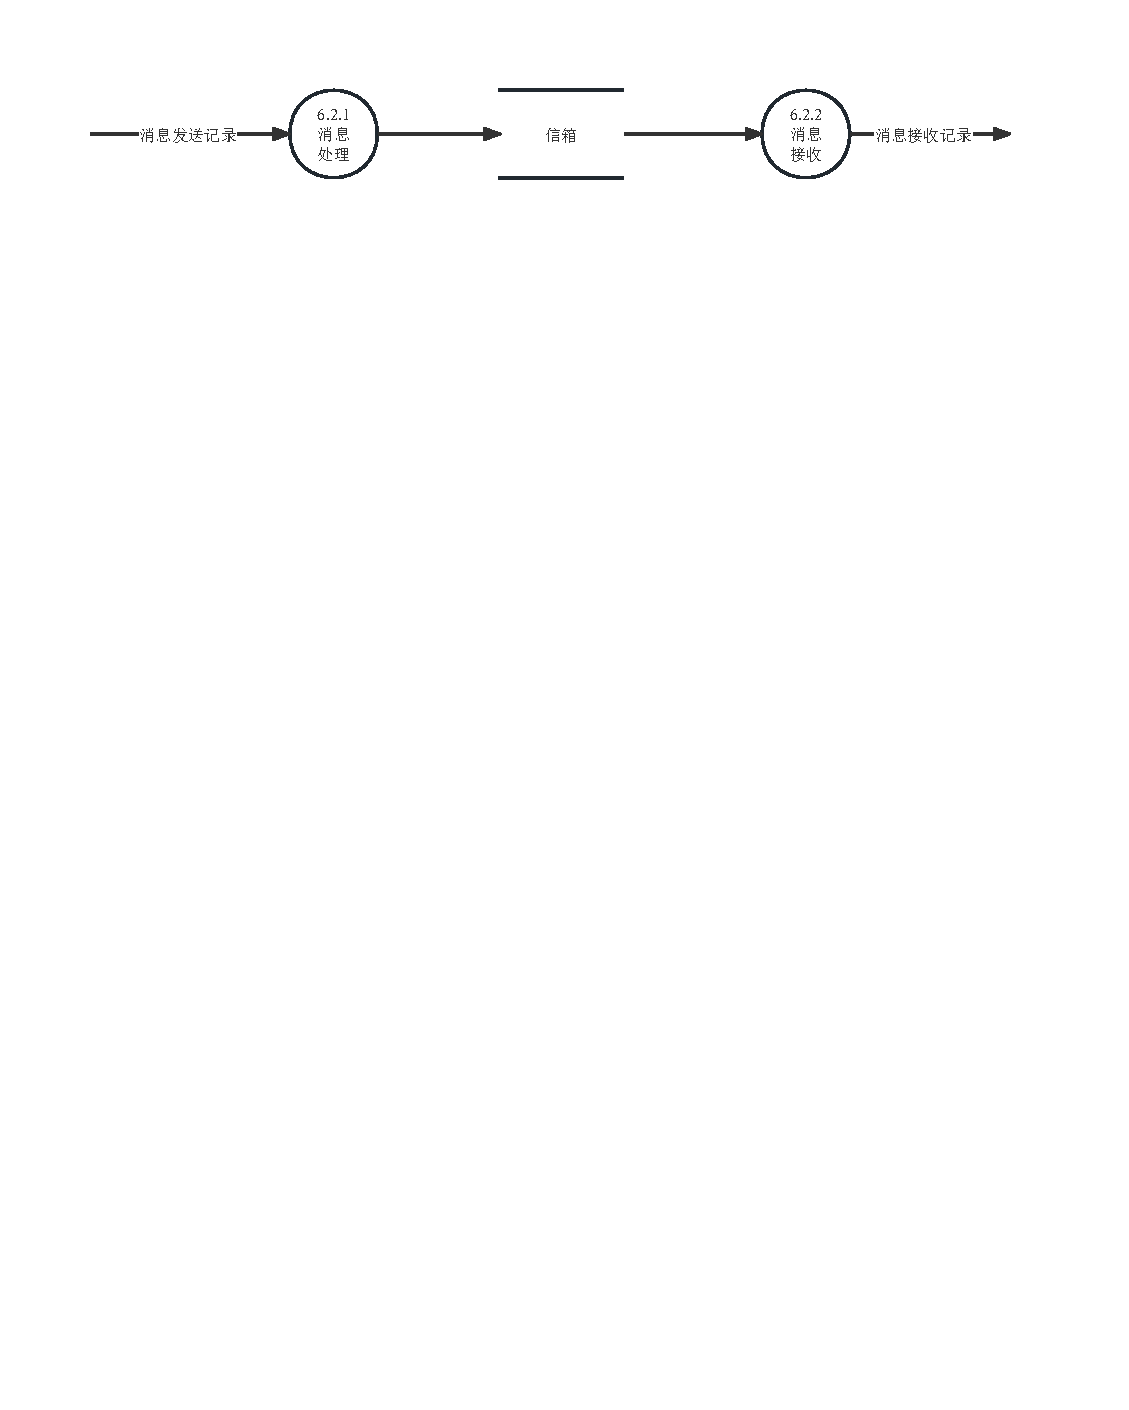
\includegraphics[width=0.95\textwidth]  {fig/社交管理/S_2-2.pdf}} 
    \bicaption{志愿交友系统2层数据流图}{Data Flow Diagram for Level 2 of Volunteer Social System}
    \end{figure}
    
(1)数据加工词条描述说明
\begin{table}[H]  
\caption{“消息发送”加工词条描述}  
\begin{center}  
    \begin{tabular}{l p{11cm}} 
        \hline
        \quad 名称:  &  消息发送 \\
        \hline
        \quad 编号:  & 6.2.1 \\
        \hline
        \quad 简述:  & 发送消息的功能 \\
        \hline
        \quad 输入:  & 消息发送记录\\
        \hline
        \quad 输出:  & 消息信息 \\
        \hline
        \quad 逻辑:  & 用户向好友发送交流信息。 \\
        \hline
    \end{tabular}
    \label{tab1}
\end{center}
\end{table}

\begin{algorithm}[H]
    \renewcommand{\thealgorithm}{}
    \caption{“消息发送”加工小说明} 
    \label{alg3} 
    \begin{algorithmic}[1]
        \STATE Get 系统时间 As 发送时间
        \STATE Generate 消息ID 
        \STATE Write 消息发送记录 + 消息ID + 发送时间 To 信箱
    \end{algorithmic} 
\end{algorithm}

\begin{table}[H]  
\caption{“消息接收”加工词条描述}  
\begin{center}  
    \begin{tabular}{l p{11cm}} 
        \hline
        \quad 名称:  &   消息接收 \\
        \hline
        \quad 编号:  & 6.2.2 \\
        \hline
        \quad 简述:  & 展示自己的所有消息 \\
        \hline
        \quad 输入:  & 消息信息 \\
        \hline
        \quad 输出:  & 消息接收记录 \\
        \hline
        \quad 逻辑:  & 返回自己收到的所有消息。 \\
        \hline
    \end{tabular}
    \label{tab1}
\end{center}
\end{table}

\begin{algorithm}[H]
    \renewcommand{\thealgorithm}{}
    \caption{“消息接收”加工小说明} 
    \label{alg3} 
    \begin{algorithmic}[1]
        \STATE Select Items In 信箱 Match 用户ID
        \STATE Write 用户ID1, 用户ID2, 消息内容 To 消息接收记录
    \end{algorithmic} 
\end{algorithm}


(2)数据流词条描述说明
\begin{table}[H]  
\caption{``消息发送记录"数据流词条描述}  
\begin{center}  
    \begin{tabular}{l p{11cm}} 
        \hline
        \quad 名称:  &   消息发送记录 \\
        \hline
        \quad 简述:  & 发送的消息记录 \\
        \hline
        \quad 来源:  & 源点``志愿者" \\
        \hline
        \quad 去向:  & 加工``消息发送" \\
        \hline
        \quad 组成:  & 用户ID1+用户ID2+消息内容 \\
        \hline
    \end{tabular}
    \label{tab1}
\end{center}
\end{table}


\begin{table}[H]  
\caption{``消息接收记录"数据流词条描述}  
\begin{center}  
    \begin{tabular}{l p{11cm}} 
        \hline
        \quad 名称:  &   消息接收记录 \\
        \hline
        \quad 简述:  & 接收的消息记录 \\
        \hline
        \quad 来源:  & 加工``消息接收" \\
        \hline
        \quad 去向:  & 源点``志愿者" \\
        \hline
        \quad 组成:  & 用户ID1+用户ID2+消息内容 \\
        \hline
    \end{tabular}
    \label{tab1}
\end{center}
\end{table}


(3)文件词条描述
\begin{table}[H]  
\caption{“信箱”文件词条描述}  
\begin{center}  
    \begin{tabular}{l p{10cm}} 
        \hline
        \quad 名称:  &   消息信息 \\
        \hline
        \quad 简述:  & 存储用户间消息信息内容\\
        \hline
        \quad 组成:  & 消息ID+用户1的ID+用户2的ID+消息内容+发送时间 \\
        \hline
        \quad 存储方式:  & 以消息ID为关键字。 \\
        \hline
    \end{tabular}
    \label{tab1}
\end{center}
\end{table}






\newpage